\documentclass[a4paper]{scrreprt}

% Uncomment to optimize for double-sided printing.
% \KOMAoptions{twoside}

% Set binding correction manually, if known.
% \KOMAoptions{BCOR=2cm}

% Localization options
\usepackage[english]{babel}
\usepackage[T1]{fontenc}
\usepackage[utf8]{inputenc}

% Quotations
\usepackage{dirtytalk}

% Enhanced verbatim sections. We're mainly interested in
% \verbatiminput though.
\usepackage{verbatim}

% PDF-compatible landscape mode.
% Makes PDF viewers show the page rotated by 90°.
\usepackage{pdflscape}

% Subfigures
\usepackage{subcaption}

% Advanced tables
\usepackage{tabu}
\usepackage{longtable}

% Fancy tablerules
\usepackage{booktabs}

% Graphics
\usepackage{graphicx}

% Current time
\usepackage[useregional=numeric]{datetime2}

% Float barriers.
% Automatically add a FloatBarrier to each \section
\usepackage[section]{placeins}

% Importing CSV into tables
\usepackage{csvsimple}

% Custom header and footer
\usepackage{fancyhdr}

\usepackage{geometry}
\usepackage{layout}

% Math tools
\usepackage{mathtools}
% Math symbols
\usepackage{amsmath,amsfonts,amssymb}
\usepackage{amsthm}

\DeclarePairedDelimiter\abs{\lvert}{\rvert}

\pagestyle{plain}
% \fancyhf{}
% \lhead{}
% \lfoot{}
% \rfoot{}
% 
% Source code & highlighting
\usepackage{listings}

% SI units
\usepackage[binary-units=true]{siunitx}
\DeclareSIUnit\Molar{\textsc{m}}
\DeclareSIUnit\Da{\textsc{Da}}
\DeclareSIUnit\mole{mol}
\DeclareSIUnit\rpm{rpm}
\DeclareSIUnit\cfu{cfu}

\usepackage{mhchem}

\newcommand{\mysubject}{2115 - Lab course biochemistry 2}
\newcommand{\mytitle}{Expression, purification and characterization of superoxide oxidase SOO}

% Convenience commands
\newcommand{\mailsubject}{\mysubject{} \mytitle{}}
\newcommand{\maillink}[1]{\href{mailto:#1?subject=\mailsubject}
                               {#1}}

% Should use this command wherever the print date is mentioned.
\newcommand{\printdate}{\today}

\subject{\mysubject{}}
\title{\mytitle{}}
\subtitle{Weeks 2 \& 3}

\author{Michael Senn \maillink{michael.senn@students.unibe.ch} - 16-126-880}

\date{\printdate}

% Needs to be the last command in the preamble, for one reason or
% another. 
\usepackage{hyperref}


\begin{document}
\maketitle

%\chapter{Procedure week 1\cite{skript_ballmoos}}

The listed steps are based on the provided script, with changes where we
deviated from what was written.

\section{Expression}

Expression was done by the assistants ahead of time, the corresponding steps of
the protocol are only listed for completeness' sake.

\begin{itemize}
	\item From a freshly transformed plate (plasmid: pET28) of the given
		membrane protein target in BL21 pLysS strain, inoculate
		\SI{30}{\ml} LB medium containing \SI{30}{\ug \per \ml}
		kanamycin (kan) for the expression of different proteins. Leave
		shaking overnight (ON) at \SI{37}{\celsius}. This pre-culture
		volume is suitable for \SI{1.5}{\l} culture grow-up.

	\item Prepare and autoclave \SI{1.5}{\l} of LB medium overnight so that
		the medium remains warm on the next day.

	\item To each \SI{1.5}{\l} bottle, add \SI{30}{\ml} of pre-culture
		inoculum, the appropriate antibiotics and incubate in a water
		bath with a controlled temperature at \SI{37}{\celsius}. We
		used a new device called LEX48 for bacteria growing in which
		shaking is replaced by air bubbling directly in the medium.

	\item Check the OD$_{\SI{600}{\nm}}$ from time to time and induce
		expression once the latter reached \numrange{1.2}{1.5} by adding
		\SI{0.2}{\milli\Molar} of IPTG (Isopropyl
		$\beta$-D-1-thiogalactopyranoside).

	\item Harvest bacterial cells 5h after induction by spinning down at
		\SI{8000}{\rpm} for \SI{15}{\min}. Discard supernatant, wash
		the pellet once with \SI{50}{\milli\Molar} HEPES pH 7.5,
		\SI{200}{\milli\Molar} \ce{NaCl}, \SI{7.5}{\percent} glycerol
		then flash-freeze in liquid nitrogen and store at
		\SI{-80}{\celsius} for further use.
\end{itemize}

In parallel, we transformed E. coli LEMO21 (DE3) strain with the plasmid
pET28-cybB561-dsred.

\begin{itemize}
	\item Plate the cells on an LB agar plate containing kanamycin and
		chloramphenicol and incubate them overnight at \SI{37}{\celsius}
\end{itemize}


\section{Isolation of membranes}

\begin{table}
	\centering
	\begin{tabu}{llll}
		\toprule
		Component & Stock & Final concentration & Used amount \\
		\midrule
		HEPES & \SI{1}{\Molar} & \SI{50}{\milli\Molar} & \SI{12.5}{\ml} \\
		Glycerol & \SI{85}{\percent} & \SI{7.5}{\milli\Molar} & \SI{22}{\ml} \\
		\ce{NaCl} & \SI{58.44}{\g \per \mole} & \SI{200}{\milli\Molar} & \SI{2.92}{\g} \\
		dd\ce{H2O} & & & To \SI{250}{\ml} \\
		\bottomrule
	\end{tabu}
	\caption{\SI{50}{\milli\Molar} HEPES buffer}
	\label{tbl:hepes_buffer}
\end{table}

\begin{table}
	\centering
	\begin{tabu}{lll}
		\toprule
		Dilution & Sample & dd\ce{H2O} \\
		\midrule
		1 : 5 & \SI{12}{\ul} & \SI{48}{\ul} \\
		1 : 10 & \SI{6}{\ul} & \SI{54}{\ul} \\
		1 : 20 & \SI{3}{\ul} & \SI{57}{\ul} \\
		1 : 40 & \SI{1.5}{\ul} & \SI{58.5}{\ul} \\
		\bottomrule
	\end{tabu}
	\caption{Sample dilutions for BCA assay}
	\label{tbl:bca_dilutions}
\end{table}

\begin{table}
	\centering
	\begin{tabu}{llll}
		\toprule Vial & Diluent & BSA & Final BSA concentration \\
		\midrule
		A & \SI{0}{\ul}   & \SI{300}{\ul} stock  & \SI{2000}{\ug\per\ml} \\
		B & \SI{125}{\ul} & \SI{375}{\ul} stock  & \SI{1500}{\ug\per\ml} \\
		C & \SI{325}{\ul} & \SI{325}{\ul} stock  & \SI{1000}{\ug\per\ml} \\
		D & \SI{175}{\ul} & \SI{175}{\ul} vial B & \SI{750}{\ug\per\ml} \\
		E & \SI{325}{\ul} & \SI{325}{\ul} vial C & \SI{500}{\ug\per\ml} \\
		F & \SI{325}{\ul} & \SI{325}{\ul} vial E & \SI{250}{\ug\per\ml} \\
		G & \SI{325}{\ul} & \SI{325}{\ul} vial F & \SI{125}{\ug\per\ml} \\
		H & \SI{400}{\ul} & \SI{100}{\ul} vial G & \SI{25}{\ug\per\ml} \\
		I & \SI{400}{\ul} & \SI{0}{\ul}          & \SI{0}{\ug\per\ml} \\
		\bottomrule
	\end{tabu}
	\caption{Standard dilutions for BCA assay}
	\label{tbl:bca_standard}
\end{table}

We worked with a bacterial pellet, weighing \SI{6.4}{\g}, containing the H158F
mutant of the superoxide oxidase.

\begin{itemize}
	\item A HEPES buffer according to table \ref{tbl:hepes_buffer} was
		prepared, the bacterial pellet thawed, and resuspended in
		\SI{32}{\ml} buffer. The resulting volume was roughly
		\SI{40}{\ml}.
	\item \SI{0.2}{\ml} of a \SI{0.2}{\Molar} PMSF stock was added for a
		final concentration of \SI{1}{\milli\Molar}
	\item \SI{0.8}{\ml} of a \SI{0.1}{\Molar} \ce{MgCl2} stock solution was
		added for a final concentration of \SI{2}{\milli\Molar}
	\item A tiny spatula tip DNAse, half a spoon lysozyme, and half a spoon
		PEFA-block were added.
	\item Bacterial cells were broken in the maximator at a pressure of $>$
		\SI{1000}{\bar}, three passes.
	\item The sample was centrifuged for \SI{15}{\min} at \SI{8000}{G} to
		remove unbroken cells and debris. The supernatant was
		transferred to a new tube, the pellet discarded. 
	\item The sample was centrifuged for \SI{5}{\min} at \SI{8000}{G} once
		more, the supernatant transferred to a new tube and the pellet
		discarded.
	\item The sample was ultracentrifuged for \SI{45}{\min} at $>$
		\SI{186000}{G} and \SI{4}{\celsius}. The supernatant was
		discarded.
	\item The pellet was resuspended in \SI{4}{\ml} HEPES buffer and
		homogenized.
	\item \SI{50}{\ul} of the sample were put aside for future use.
	\item Four dilutions according to table \ref{tbl:bca_dilutions} were
		prepared.
	\item The BCA working reaction was prepared by another group.
	\item Four tubes were prepared, each containing \SI{50}{\ul} of one of
		the dilutions and \SI{950}{\ul} of the BCA working reaction.
	\item The BCA assays were incubated for \SI{15}{\min} at \SI{37}{\celsius}
	\item A standard curve based on BSA was prepared by another group,
		according to table \ref{tbl:bca_standard}.
	\item The absorption of the dilutions and the standard curve at
		\SI{562}{\nm} was measured. % TODO link table?
\end{itemize}

\section{Preparation of transformed pre-culture}

The following steps were performed by another group, and are listed for
completeness' sake.

\begin{itemize}
	\item Pick 3 colonies from a freshly transformed plate with plasmid
		pET28a-cybB561-dsred of the given membrane protein target in
		Lemo21 (DE3) strain and inoculate \SI{15}{\ml} LB-medium
		containing \SI{35}{\ug \per \ml} of kanamycin (kan) and
		\SI{25}{\ug \per \ml} of chloramphenicol.
	\item Leave shaking overnight (ON) at \SI{37}{\celsius}. This volume is
		suitable for optimization of protein expression experiments
		(day 2)
\end{itemize}

In addition, medium according to tables \ref{tbl:medium_lb},
\ref{tbl:medium_tb_1}, \ref{tbl:medium_tb_2}, \ref{tbl:medium_auto_basis} and
\ref{tbl:medium_auto_stock} were prepared.

The LB medium was autoclaved. Part 1 of the TB medium was autoclaved, part 2
filtered. Both parts of the auto-inducing medium had their pH set to 7 with
\ce{NaOH}, the basis was then autoclaved and the stock filtered. All medium was
then set aside for the next day.

\begin{table}
	\centering
	\begin{tabu}{llll}
		\toprule
		Component & Stock & Final concentration & Used amount \\
		\midrule
		Tryptone & & \SI{1}{\percent} & \SI{2}{\g} \\
		Yeast extract & & \SI{0.5}{\percent} & \SI{1}{\g} \\
		\ce{NaCl} & & \SI{0.5}{\percent} & \SI{1}{\g} \\
		\ce{H2O} & & & To \SI{200}{\ml} \\
		\bottomrule
	\end{tabu}
	\caption{LB medium}
	\label{tbl:medium_lb}
\end{table}

\begin{table}
	\centering
	\begin{tabu}{llll}
		\toprule
		Component & Stock & Final concentration & Used amount \\
		\midrule
		Tryptone & & \SI{1.2}{\percent} & \SI{2.4}{\g} \\
		Yeast extract & & \SI{2.4}{\percent} & \SI{4.8}{\g} \\
		\ce{H2O} & & & To \SI{180}{\ml} \\
		\bottomrule
	\end{tabu}
	\caption{TB medium part 1}
	\label{tbl:medium_tb_1}
\end{table}

\begin{table}
	\centering
	\begin{tabu}{llll}
		\toprule
		Component & Stock & Final concentration & Used amount \\
		\midrule
		\ce{KH2PO4} & & \SI{17}{\milli\Molar} & \SI{0.46}{\g} \\
		\ce{K2HPO4} & & \SI{72}{\milli\Molar} & \SI{1.25}{\g} \\
		\ce{Glycerol} & \SI{85}{\percent} & \SI{0.5}{\percent} & \SI{588}{\ul} \\
		\ce{H2O} & & & To \SI{20}{\ml} \\
		\bottomrule
	\end{tabu}
	\caption{TB medium part 2}
	\label{tbl:medium_tb_2}
\end{table}

\begin{table}
	\centering
	\begin{tabu}{llll}
		\toprule
		Component & Stock & Final concentration & Used amount \\
		\midrule
		Tryptone & & \SI{1}{\percent} & \SI{2}{\g} \\
		Yeast extract & & \SI{0.5}{\percent} & \SI{1}{\g} \\
		\ce{H2O} & & & To \SI{180}{\ml} \\
		\bottomrule
	\end{tabu}
	\caption{Auto-inducing medium basis}
	\label{tbl:medium_auto_basis}
\end{table}

\begin{table}
	\centering
	\begin{tabu}{llll}
		\toprule
		Component & Stock & Final concentration & Used amount \\
		\midrule
		\ce{Na2HPO4} & & \SI{500}{\milli\Molar} & \SI{2.67}{\g} \\
		\ce{KH2PO4} & & \SI{500}{\milli\Molar} & \SI{2.04}{\g} \\
		\ce{(NH4)2SO4} & & \SI{250}{\milli\Molar} & \SI{1}{\g} \\
		\ce{MgSO4} & \SI{1}{\Molar} & \SI{20}{\milli\Molar} & \SI{600}{\ul} \\
		\ce{Glycerol} & \SI{85}{\percent} & \SI{5}{\percent} & \SI{1.76}{\ml} \\
		\ce{Glucose} & & \SI{0.5}{\percent} & \SI{0.16}{\g} \\
		\ce{Lactose} & & \SI{2}{\percent} & \SI{0.6}{\g} \\
		\ce{H2O} & & & To \SI{30}{\ml} \\
		\bottomrule
	\end{tabu}
	\caption{Auto-inducing medium 10x stock}
	\label{tbl:medium_auto_stock}
\end{table}


\section{Transformation of bacterial cells}

\begin{itemize}
	\item \SI{50}{\ul} of \ce{CaCl2} treated competent cells were mixed
		with \SI{1}{\ul} of pET28-cybB561 plasmids and incubated on ice
		for \SI{30}{\min}.
	\item The mixture was heat-shocked for \SI{1}{\min} at
		\SI{42}{\celsius}, then incubated on ice for \SI{5}{\min}.
	\item \SI{0.5}{\ml} LB medium, pre-warmed to \SI{37}{\celsius}, was
		added.
	\item The mixture was incubated for \SI{1}{\hour} at \SI{37}{\celsius}.
	\item The transformed bacteria were spread on a LB plate containing
		\SI{30}{\ug\per\ml} kanamycin.
	\item The plate was incubated overnight at \SI{37}{\celsius}.
	\item On the next day bacterial growth was observed on the plate,
		indicating that the transformation had been successful. The
		plate was then discarded.
\end{itemize}

\section{Expression screening of E. coli cells}

\begin{itemize}
	\item The two parts of the TB and auto-inducing medium respectively
		were mixed.
	\item Antibiotics were added to all media.
		\begin{itemize}
			\item \SI{200}{\ul} kanamycin of a \SI{35}{\mg\per\ml}
				stock for a final concentration of
				\SI{35}{\ug\per\ml}.
			\item \SI{200}{\ul} chloramphenicol of a
				\SI{25}{\mg\per\ml} stock for a final
				concentration of \SI{25}{\ug\per\ml}.
		\end{itemize}
	\item \SI{1}{\ml} of each medium was set aside for use as a blank.
	\item Samples according to table \ref{tbl:expression_samples} were
		prepared.
		\begin{itemize}
			\item All samples had \SI{15}{\ml} of its corresponding
				medium, and \SI{800}{\ul} of the preculture
				added.
			\item All Rha+ samples had \SI{37.5}{\ul} of a
				\SI{0.1}{\Molar} Rhamnose stock solution added,
				for a final concentration of
				\SI{0.25}{\milli\Molar}.
		\end{itemize}
	\item Samples were incubated at \SI{37}{\celsius}, and their OD$_{600}$
		measured every \SIrange{30}{60}{\min} until their absorbance had
		reached $0.5$.

		The measurement at \SI{90}{\min} was later found to be
		incorrect due to the cuvette having been inserted the wrong
		way.

	\item After \SI{90}{\min} all IPTG+ samples had \SI{13}{\ul} of a
		\SI{0.2}{\Molar} stock solution added.
	\item Samples were incubated at \SI{37}{\celsius} for another
		\SI{200}{\min}, and had their OD$_{600}$ measured every
		\SIrange{30}{90} minutes. The volume used to measure the
		absorbance of the LB samples was subsequently centrifuged, and
		the size and colour of the pellet observed.
	\item After \SI{290}{\min} \SI{198}{\ul} of the culture were
		solubilized with \SI{2}{\ml} of a \SI{10}{\percent} SDS stock
		solution in a 96-well plate. The fluorescence was measured with
		a plate reader to determine the amount of expressed protein. The
		measurements for the LB samples were redone, as they had been
		contaminated while being added to the well.
% TODO: Link table with measurements?
\end{itemize}

\begin{table}
	\centering
	\begin{tabu}{lll}
		\toprule
		Medium & Rhamnose & IPTG \\
		\midrule
		LB & - & - \\
		LB & + & - \\
		LB & - & + \\
		LB & + & + \\

		TB & - & - \\
		TB & + & - \\
		TB & - & + \\
		TB & + & + \\

		ZYM-505 & - & - \\
		ZYM-505 & + & - \\
		ZYM-505 & - & + \\
		ZYM-505 & + & + \\
		\bottomrule
	\end{tabu}
	\caption{Samples for protein expression screening}
	\label{tbl:expression_samples}
\end{table}


\chapter{Procedure week 2 \& 3}

\section{Purification}

\subsection{Memrane solubilization}

\begin{itemize}
	\item Thaw membranes (\SI{10}{\mg\per\ml}) that you prepared on the
		first day.
	\item Create \SI{11}{\ml} dilution according to table
		\ref{tbl:membrane_dilution}
	\item Incubate mixture at \SI{4}{\celsius} for \SI{1}{\hour} while
		stirring slowly.
	\item During solubilisation, prepare buffers used for purification.
	\item Pellet the insolubilized membrane by ultracentrifugation at
		\SI{150000}{G} (Ti60-Rotor: 46000rpm) for \SI{45}{\min} at
		\SI{4}{\celsius}.
	\item Prepare HEPES wash buffer according to table
		\ref{tbl:hepes_buffer_no_ogng}, adjust pH to 7. Split in two
		\SI{250}{\ml} flasks, add \SI{10}{\percent} OGNG to one.
	\item Load \SI{2}{\ml} of Profinity beads on the column.
	\item Once ethanol is removed, add \SI{10}{\ml} (10 column volumes) of
		\SI{50}{\milli\Molar} Sodium acetate pH4,
		\SI{300}{\milli\Molar} \ce{NaCl}.
	\item Load \SI{10}{\ml} of \SI{0.2}{\Molar} Nickel (10 column volumes) 
	\item Wash the column with \SI{10}{\ml} (10 column volumes) of
		\SI{50}{\milli\Molar} Sodium acetate pH4,
		\SI{300}{\milli\Molar} \ce{NaCl}.
	\item Wash the column with \SI{15}{\ml} of MQ water
	\item Equilibrate the resin with \SI{15}{\ml} of wash buffer
		(\SI{10}{\milli\Molar} HEPES pH 7, \SI{200}{\milli\Molar}
		\ce{NaCl}, \SI{5}{\percent} glycerol and \SI{0.1}{\percent}
		OGNG. The Ni-beads are now ready to use.
\end{itemize}

\subsection{Protein purification}

\begin{itemize}
	\item Prepare \SI{40}{\ml} wash buffer with \SI{5}{\milli\Molar}
		Histidine, and \SI{80}{\ml} wash buffer with
		\SI{100}{\milli\Molar} Histidine.
	\item Mix the supernatant with Ni-beads and incubate for \SI{45}{\min}
		at \SI{4}{\celsius} on a rotating wheel.
	\item Load the slurry on the column and collect the flowthrough
		(unbound proteins).
	\item Let flowthrough pass through resin 1 more time in order to bind
		remaining His-tagged protein. Keep an aliquot of \SI{12}{\ul}
		on ice. For cybB561-dsred, keep \SI{30}{\ul}.
	\item Wash the column with \SI{10}{\ml} (10 column volumes) of wash
		buffer containing OGNG. Keep an aliquot of \SI{12}{\ul} on ice.
		For cybB561-dsred, keep \SI{30}{\ul}.
	\item Wash the column with \SI{10}{\ml} (10 column volumes) of wash
		buffer \SI{5}{\milli\Molar} Histidine. Keep an aliquot of
		\SI{12}{\ul} on ice. For cybB561-dsred, keep \SI{30}{\ul}. Why
		do we wash with \SI{5}{\milli\Molar} histidine?
	\item Elute the column with \SI{20}{\ml} wash buffer +
		\SI{100}{\milli\Molar} Histidine. Keep an aliquot of
		\SI{12}{\ul} on ice. For cybB561-dsred, keep \SI{30}{\ul}.
	\item Concentrate the eluate with an Amicon \SI{10}{\kilo\Da} MWCO
		centrifugal concentrator to \SI{0.5}{\ml} (volume needed to
		inject on the size exclusion chromatography column S200
		increase).
\end{itemize}


Only for cybB561-Dsred protein, we will try to separate CybB561 and Dsred in
presence of TEV protease.

\begin{itemize}
	\item take \SI{100}{\ul} of the concentrated CybB561-Dsred and dilute
		it in \SI{10}{\ml} of \SI{10}{\milli\Molar} HEPES pH7,
		\SI{200}{\milli\Molar} \ce{NaCl}, \SI{5}{\percent} glycerol,
		\SI{0.1}{\percent} OGNG.
	\item Add \SI{200}{\ul} of TEV protease (\SI{1}{\mg\per\ml},
		M=\SI{25}{\kilo\Da}, final concentration =
		\SI{0.8}{\micro\Molar})
	\item Incubate overnight at \SI{4}{\celsius} and mix with magnetic
		stirrer.
\end{itemize}



\subsection{Size exclusion chromatography}

After purification of protein of interest using affinity chromatography, you will purify the concentrated protein again using size exclusion chromatography (gel filtration). What is the reason behind this additional step?

\begin{itemize}
	\item S200 column equilibrated overnight using wash buffer with OGNG.
	\item Fill the loop (\SI{0.5}{\ml}) on the ÄKTA pure device with the
		concentrated samples (\SI{0.5}{\ml}).
	\item Start the run. Note that fractions of eluted proteins will be
		collected automatically.
	\item Pool together fractions that you suspect to contain the protein
		of interest.
	\item Concentrate with an Amicon \SI{10}{\kilo\Da} MWCO centrifugal
		concentrator (final volume that can be reached is
		\SI{250}{\ul}).
\end{itemize}

\subsection{Reverse IMAC}

While running a gel filtration, you will do a reverse IMAC with cybB561.Dsred
cleaved overnight using TEV protease as follows:

\begin{itemize}
	\item First, take a sample of \SI{30}{\ul}, keep on ice.
	\item Load the mixture on the column (containing pre-equilibrated resin
		charged again with nickel).
	\item Retain the flow-through. Keep an aliquot of \SI{30}{\ul} on ice.
		Flowthrough was kept as it contained the cleaved HS. The
		flowthrough was light red, the beads not red.
	\item Load elution buffer on the column (the same that you used a day
		before). Keep an aliquot of \SI{30}{\ul} on ice. The elution
		was pink.
\end{itemize}

\subsection{Protein concentration determination}

To determine the concentration of the different purified proteins, we will take
advantage of the absorbance of the 2 hemes that are buried inside the protein.

\begin{itemize}
	\item A buffer \SI{20}{\milli\Molar} HEPES pH7.4, \SI{20}{\milli\Molar}
		\ce{KCl} \SI{200}{\milli\Molar} \ce{NaCl}, \SI{0.05}{\percent}
		DDM was prepared.
	\item A cuvette was filled with \SI{748}{\ul} buffer and the baseline measured by scanning between \SI{600}{\nm} and \SI{400}{\nm}.
	\item \SI{2}{\ul} of protein were added and measured again.
	\item A small amount of sodium dithionite was added to fully reduce the
		protein, and another measurement done.
	\item The original protein concentration was calculated using the
		dilution factor, baseline-compensanted \SI{561}{\nm} absorbance
		difference of oxidized and reduced form, path length of
		\SI{1}{\c} and and extinction coefficient of
		\SI{46.36}{\per\milli\Molar\per\cm}.
	\item Proteins were frozen in liquid nitrogen in small droplets, and
		stored at \SI{-80}{\celsius}.
\end{itemize}

\subsection{SDS-PAGE}

\begin{itemize}
	\item Two gels were prepared according to the recipe (\SI{12}{\percent}).
	\item Samples were prepared according to table \ref{tbl:sds_samples}.
	\item Samples were incubated for \SI{30}{\min} at \SI{40}{\celsius}
	\item \SI{10}{\ul} of sample were loaded per lane, with \SI{5}{\ul} ruler in empty lanes.
	\item The gel was run for \SI{20}{\min} at \SI{125}{\V}, followed by \SI{80}{\min} at \SI{185}{\V}.
	\item The gel was coomassie-stained, and cleaned overnight.
\end{itemize}


\subsection{Fluorescence measurements}

The efficiency of each purification step can be determined by the measurement
of fluorescence of the different samples that were taken in different steps of
purification (this can only be done for cybB561-dsred).

\begin{itemize}
	\item \SI{15}{\ul} of each sample were diluted to \SI{200}{\ul} with
		dd\ce{H2O}.
	\item Diluated samples were loaded onto a 96-well plate.
	\item Fluorescence was measured at an emission of \SI{586}{\nm},
		extinction of \SI{555}{\nm}
\end{itemize}

\begin{table}
	\centering
	\begin{tabu}{llll}
		\toprule
		Component & Stock & Final concentration & Used amount \\
		\midrule
		H158F & \SI{20}{\mg\per\ml} & \SI{10}{\mg\per\ml} & \SI{5.5}{\ml} \\
		OGNG & \SI{9}{\percent} & \SI{1}{\percent} & \SI{12}{\ml} \\
		Glycerol & \SI{85}{\percent} & \SI{5}{\percent} & \SI{0.647}{\ml} \\
		PMSF & \SI{1}{\milli\Molar} & \SI{200}{\milli\Molar} & \SI{55}{\ul} \\
		PEF block & & & some crystals \\
		HEPES Buffer & & & \SI{3.598}{\ml} \\
		\bottomrule
	\end{tabu}
	\caption{\SI{11}{\ml} Membrane dilution}
	\label{tbl:membrane_dilution}
\end{table}

\begin{table}
	\centering
	\begin{tabu}{llll}
		\toprule
		Component & Stock & Final concentration & Used amount \\
		\midrule
		HEPES & \SI{1}{\Molar} & \SI{10}{\milli\Molar} & \SI{5}{\ml} \\
		\ce{NaCl} & \SI{2}{\Molar} & \SI{200}{\milli\Molar} & \SI{50}{\ml} \\
		Glycerol & \SI{85}{\percent} & \SI{5}{\percent} & \SI{29.4}{\ml} \\
		PMSF & \SI{1}{\milli\Molar} & \SI{200}{\milli\Molar} & \SI{55}{\ul} \\
		dd \ce{H2O} & & & \SI{410.05}{\ml} \\
		\bottomrule
	\end{tabu}
	\caption{\SI{50}{\ml} wash buffer}
	\label{tbl:hepes_buffer_no_ogng}
\end{table}

\begin{table}
	\centering
	\begin{tabu}{llllll}
		\toprule
		Gel & Lane & Sample & Protein & Buffer & dd\ce{H2O} \\
		\midrule
		1 & 1 & Ladder & \SI{5}{\ul} & - & - \\
		1 & 2 & wt Flowthrough & \SI{3}{\ul} & \SI{3}{\ul} & \SI{9}{\ul} \\
		1 & 3 & wt Wash & \SI{12}{\ul} & \SI{3}{\ul} & \SI{0}{\ul} \\
		1 & 4 & wt Wash \SI{5}{\milli\Molar} His & \SI{12}{\ul} & \SI{3}{\ul} & \SI{0}{\ul} \\
		1 & 5 & wt before ÄKTA (conc) & \SI{1}{\ul} & \SI{3}{\ul} & \SI{11}{\ul} \\
		1 & 6 & wt after ÄKTA (conc) & \SI{0.5}{\ul} & \SI{3}{\ul} & \SI{11.5}{\ul} \\

		1 & 7 & Ladder & \SI{5}{\ul} & - & - \\
		1 & 8 & mt Flowthrough & \SI{3}{\ul} & \SI{3}{\ul} & \SI{9}{\ul} \\
		1 & 9 & mt Wash & \SI{12}{\ul} & \SI{3}{\ul} & \SI{0}{\ul} \\
		1 & 10 & mt Wash \SI{5}{\milli\Molar} His & \SI{12}{\ul} & \SI{3}{\ul} & \SI{0}{\ul} \\
		1 & 11 & mt before ÄKTA (conc) & \SI{1}{\ul} & \SI{3}{\ul} & \SI{11}{\ul} \\
		1 & 12 & mt after ÄKTA (conc) & \SI{0.5}{\ul} & \SI{3}{\ul} & \SI{11.5}{\ul} \\
		1 & 13 & & & & \\
		1 & 14 & Used by assistant & & & \\


		2 & 1 & Ladder & \SI{5}{\ul} & - & - \\
		2 & 2 & dsRed Flowthrough & \SI{3}{\ul} & \SI{3}{\ul} & \SI{9}{\ul} \\
		2 & 3 & dsRed Wash & \SI{12}{\ul} & \SI{3}{\ul} & \SI{0}{\ul} \\
		2 & 4 & dsRed Wash \SI{5}{\milli\Molar} His & \SI{12}{\ul} & \SI{3}{\ul} & \SI{0}{\ul} \\
		2 & 5 & dsRed before ÄKTA (conc) & \SI{1}{\ul} & \SI{3}{\ul} & \SI{11}{\ul} \\
		2 & 6 & dsRed after ÄKTA (conc) & \SI{0.5}{\ul} & \SI{3}{\ul} & \SI{11.5}{\ul} \\
		2 & 7 & dsRed flowthrough (conc) & \SI{1}{\ul} & \SI{3}{\ul} & \SI{11}{\ul} \\
		2 & 8 & dsRed before ÄKTA (conc) & \SI{1}{\ul} & \SI{3}{\ul} & \SI{11}{\ul} \\
		2 & 9 & dsRed cleaved before loading & \SI{12}{\ul} & \SI{3}{\ul} & \SI{0}{\ul} \\
		2 & 10 & dsRed cleaved flowthrough & \SI{12}{\ul} & \SI{3}{\ul} & \SI{0}{\ul} \\
		2 & 11 & dsRed cleaved elution & \SI{12}{\ul} & \SI{3}{\ul} & \SI{0}{\ul} \\
		2 & 12 & TEV & \SI{2}{\ul} & \SI{3}{\ul} & \SI{10}{\ul} \\
		2 & 13 & wt after ÄKTA & \SI{0.5}{\ul} & \SI{3}{\ul} & \SI{11.5}{\ul} \\
		2 & 14 & dsRed & \SI{8}{\ul} & \SI{3}{\ul} & \SI{4}{\ul} \\
		\bottomrule
	\end{tabu}
	\caption{SDS-PAGE samples}
	\label{tbl:sds_samples}
\end{table}




%\chapter{Results week 1}

\section{Protein concentration via BCA assay}

\label{sec:protein_concentration}

The measured absorption values at \SI{562}{\nm} of the prepared standard are
shown in table \ref{tbl:bca_absorption_standard}. Based on those, the device
calculated a linear regression:

\[
	\text{absorption} = 0.81542 \cdot \text{concentration} + 0.02701
\]

This allows calculating the concentration of the diluted samples based on their
absorption values, shown in table \ref{tbl:bca_absorption_sample}.

The measured absorption values of the standard and sample dilutions, as well as
their known respectively calculated concentrations, is further visualized in
figure \ref{fig:bca_absorption}.

Discarding the two measurements which fall outside the range of the standard,
and calculating the protein concentration of the undiluted sample, yields
concentrations of \SI{21.552}{\mg\per\ml} and \SI{17.342}{\mg\per\ml}
respectively. Using their average provides us with a protein concentration of
\SI{19.447}{\mg\per\ml}.

\begin{table}
	\centering
	\begin{tabu}{ll}
		\toprule
		Absorption & Concentration (known) \\
		\midrule
		\SI{1.6353}{OD562} & \SI{2000}{\ug\per\ml} \\
		\SI{1.2418}{OD562} & \SI{1500}{\ug\per\ml} \\
		\SI{0.8755}{OD562} & \SI{1000}{\ug\per\ml} \\
		\SI{0.6433}{OD562} & \SI{750}{\ug\per\ml} \\
		\SI{0.4756}{OD562} & \SI{500}{\ug\per\ml} \\
		\SI{0.2413}{OD562} & \SI{250}{\ug\per\ml} \\
		\SI{0.1173}{OD562} & \SI{125}{\ug\per\ml} \\
		\SI0.0225{}{OD562} & \SI{25}{\ug\per\ml} \\
		\SI{0.0053}{OD562} & \SI{0}{\ug\per\ml} \\
		\bottomrule
	\end{tabu}
	\caption{OD562 values of standard}
	\label{tbl:bca_absorption_standard}
\end{table}

\begin{table}
	\centering
	\begin{tabu}{lll}
		\toprule
		Absorption & Concentration (calculated) & Dilution factor \\
		\midrule
		\SI{2.2966}{OD562} & \SI{2783}{\ug\per\ml} & 1:5 \\
		\SI{1.8855}{OD562} & \SI{2279}{\ug\per\ml} & 1:10 \\
		\SI{0.8671}{OD562} & \SI{1030}{\ug\per\ml} & 1:20 \\
		\SI{0.5388}{OD562} & \SI{628}{\ug\per\ml} & 1:40 \\
		\bottomrule
	\end{tabu}
	\caption{OD562 values of sample dilutions}
	\label{tbl:bca_absorption_sample}
\end{table}

\begin{figure}
	\centering
	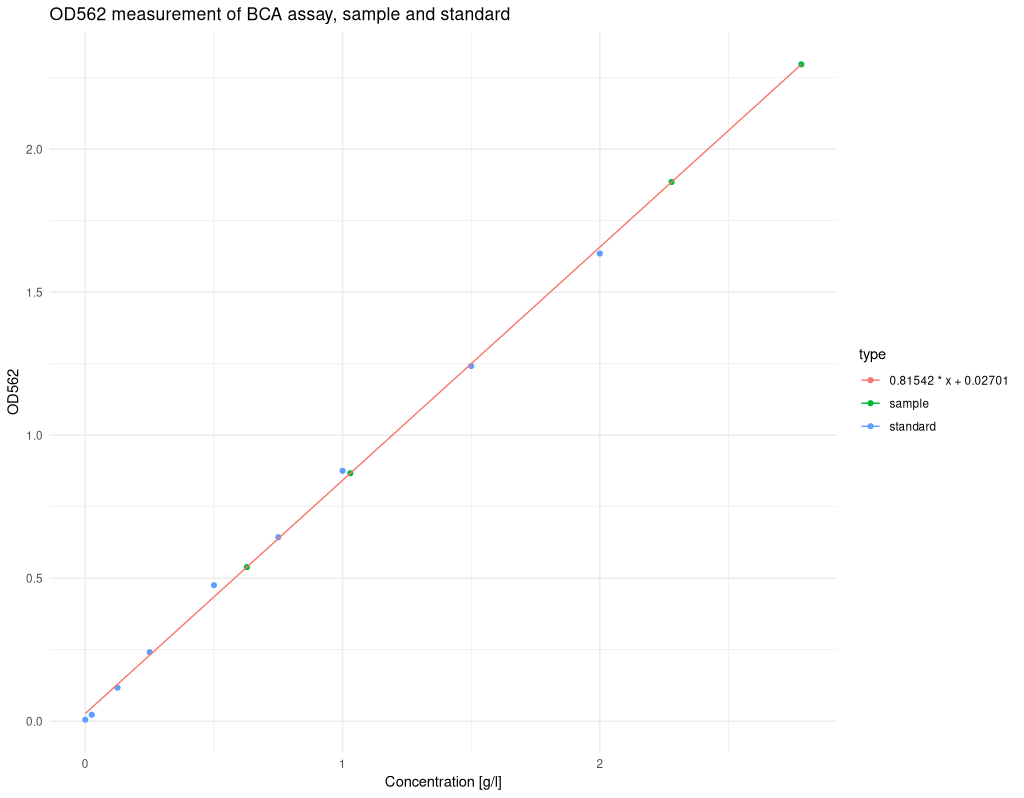
\includegraphics[width=\linewidth]{img/bca_assay.png}
	\caption{OD562 values and concentrations of standard and sample}
	\label{fig:bca_absorption}
\end{figure}

\section{Expression screening}

\subsection{OD measurements during bacterial growth}

To measure the stages of bacterial growth before and after induction, the
absorption at \SI{600}{\nm} was measured in regular intervals. These results are
found in table \ref{tbl:absorption_expression}.

As mentioned in the protocol the measurement at \SI{90}{\min} was faulty, and
was thus excluded from the visualization in figure
\ref{fig:absorption_expression}.

\begin{table}
	\centering
	\begin{tabu}{lllllllll}
		\toprule
		Medium & Rha & IPTG & \SI{0}{\min} & \SI{60}{\min} & \SI{90}{\min} & \SI{120}{\min} & \SI{200}{\min} & \SI{290}{\min} \\
		\midrule
		\csvreader[]{data/expression_od600.csv}%
		{medium=\medium,rha=\rha,iptg=\iptg,4=\tone,5=\ttwo,6=\tthree,7=\tfour,8=\tfive,9=\tsix}%
		{\\ \medium & \rha & \iptg & \tone & \ttwo& \tthree & \tfour & \tfive & \tsix}%
		\\
		\bottomrule
	\end{tabu}
	\caption{OD600 values of transformed bacteria samples}
	\label{tbl:absorption_expression}
\end{table}

\begin{figure}
	\centering
	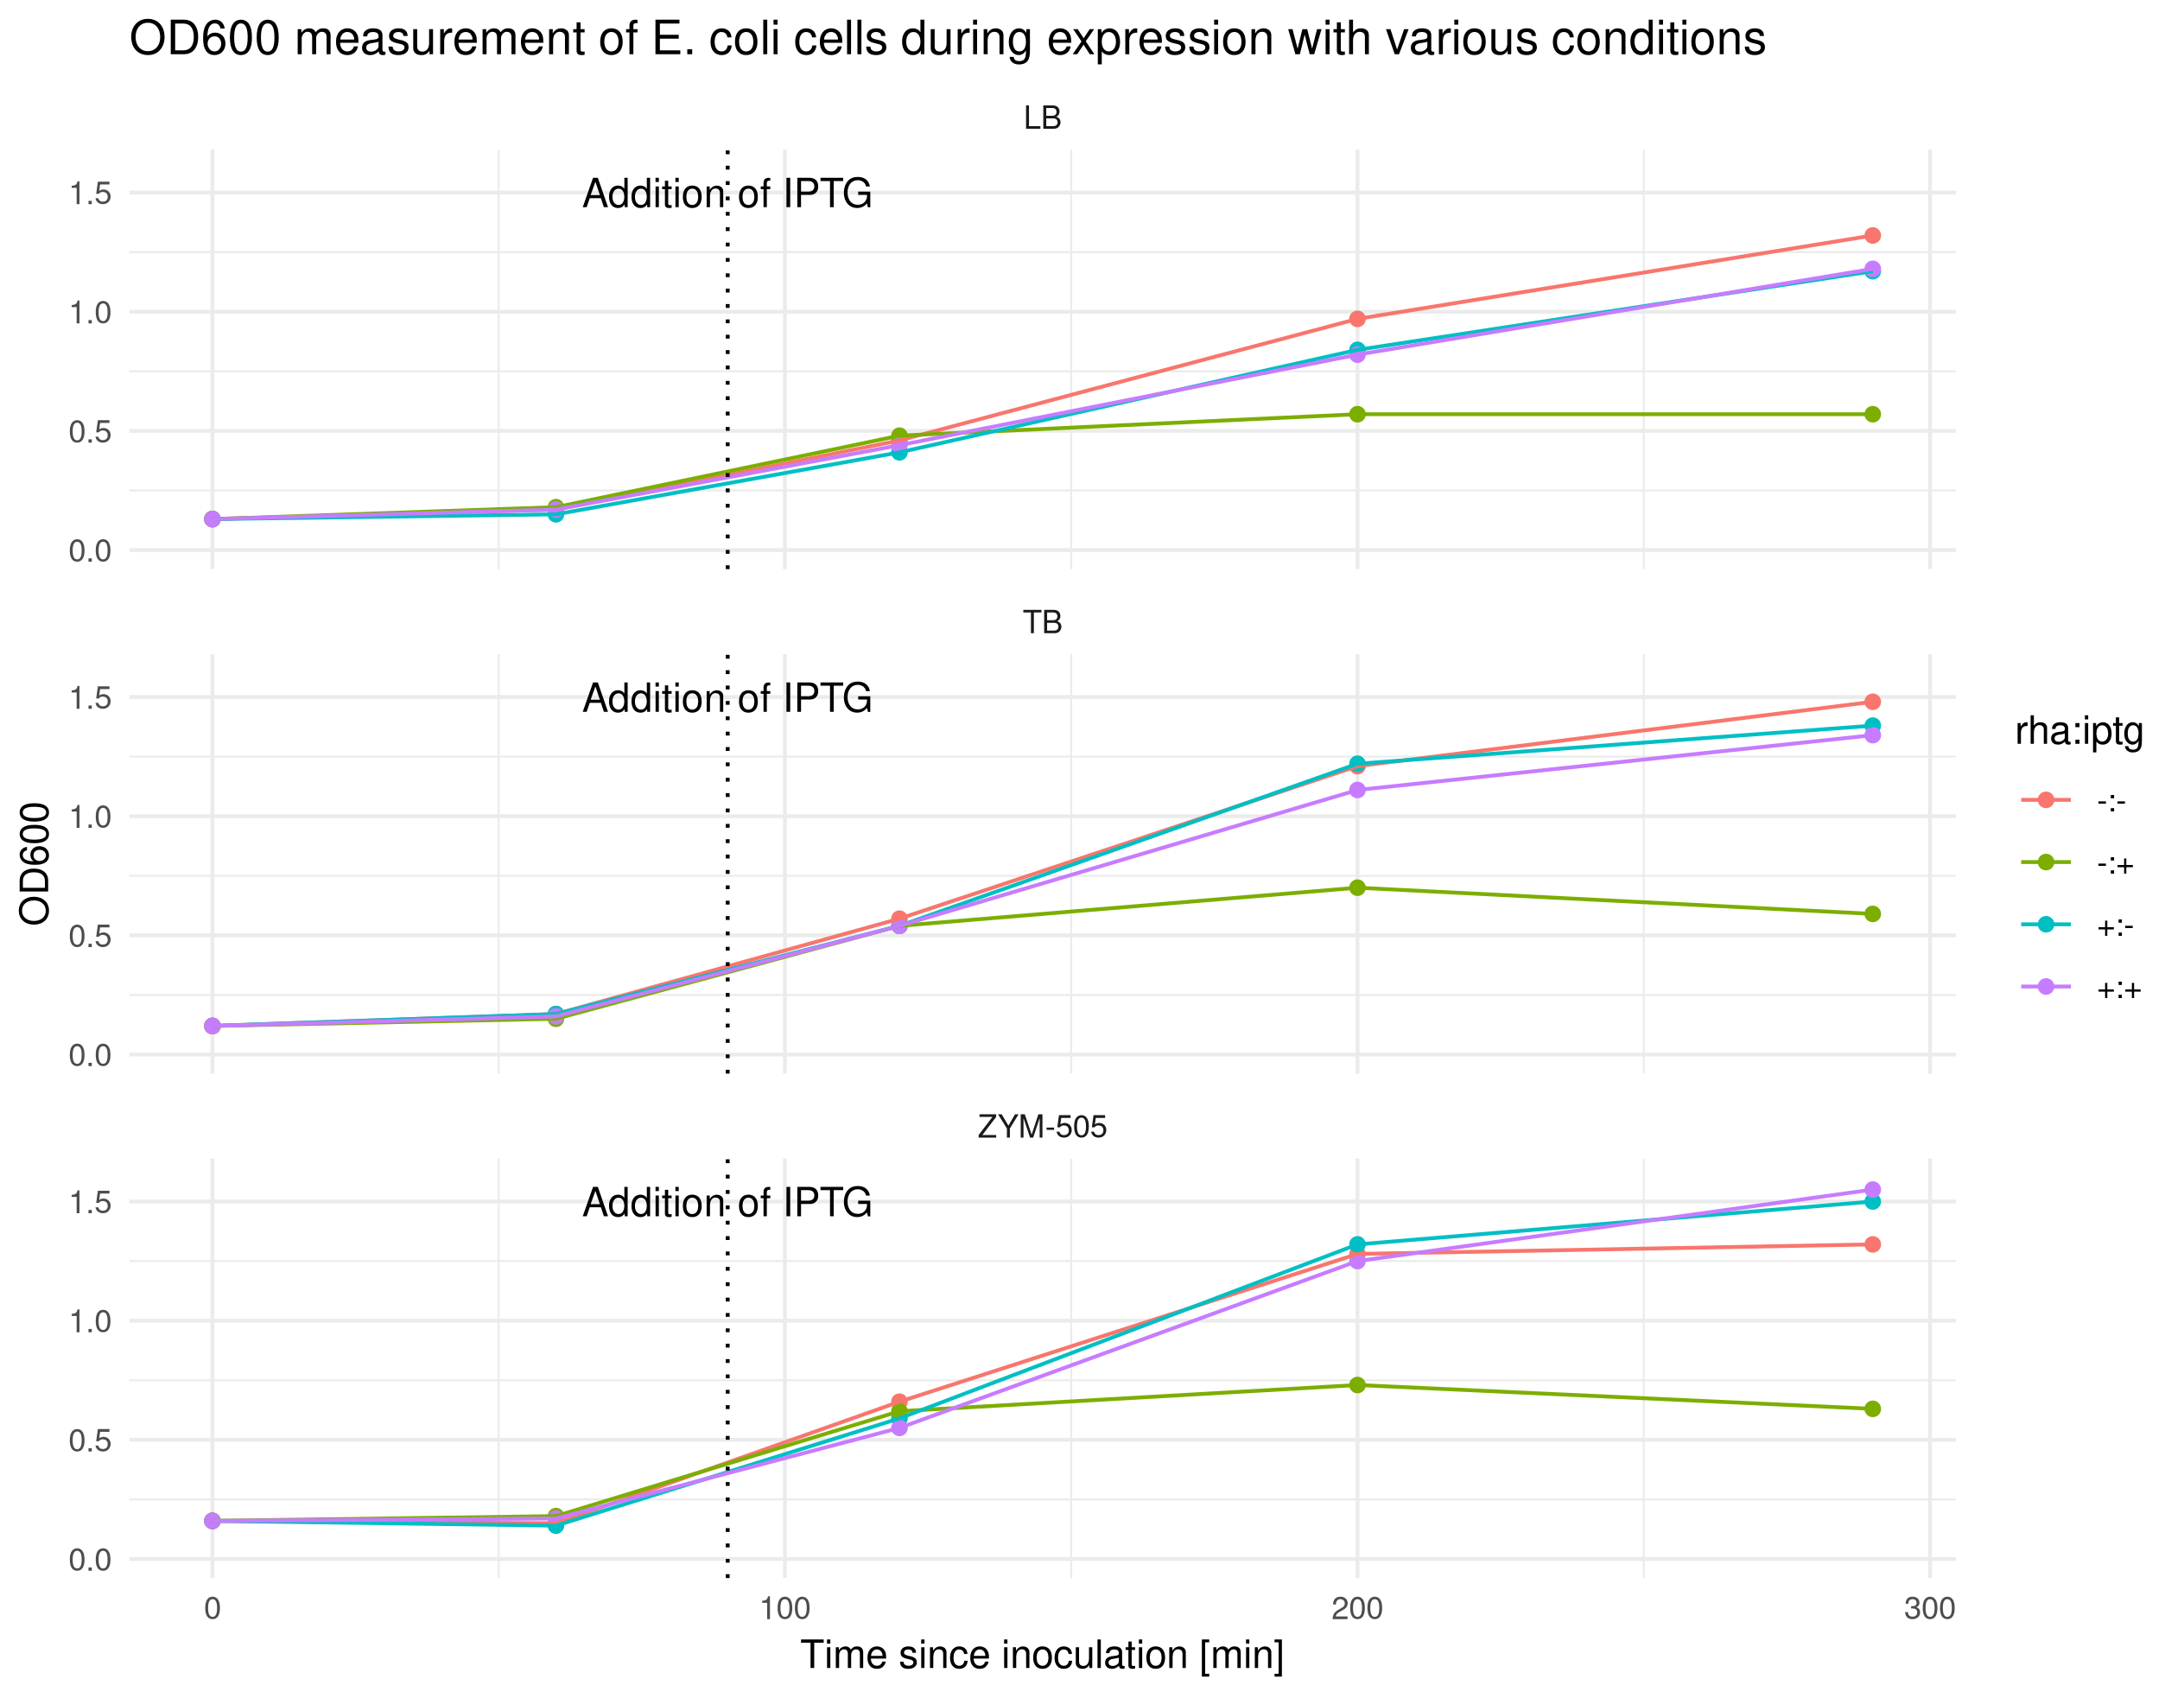
\includegraphics[width=\linewidth]{img/absorption_expression.png}
	\caption{OD600 values over time of expression samples}
	\label{fig:absorption_expression}
\end{figure}

\subsection{Fluorescence measurement}

The fluorescence measurements of the dsRed-marked protein are shown in table
\ref{tbl:expression_fluorescence}. In addition to the measured value this table
also includes the fluorescence normalized to an OD of 1, using the most recent
OD measurements. These values are further visualized in figure
\ref{fig:expression_fluorescence}.

\begin{table}
	\centering
	\begin{tabu}{llllll}
		\toprule
		Medium & Rha & IPTG & Fluorescence & Last OD$_{600}$ & Normalized fluorescence \\
		\midrule
		\csvreader[]{data/expression_fluorescence.csv}%
		{Medium=\medium,Rhamnose=\rha,IPTG=\iptg,Fluorescence=\fluorescence,5=\od,6=\fluorescencenorm}%
		{\\ \medium & \rha & \iptg & \fluorescence & \od & \fluorescencenorm}%
		\\
		\bottomrule
	\end{tabu}
	\caption{Fluorescence values of transformed bacteria samples}
	\label{tbl:expression_fluorescence}
\end{table}

\begin{figure}
	\centering
	\includegraphics[width=\linewidth]{img/expression_fluorescence.png}
	\caption{Fluorescence values of transformed bacteria samples}
	\label{fig:expression_fluorescence}
\end{figure}


%\chapter{Discussion week 1}

\section{Isolation of membranes}

The relatively big difference of roughly \SI{20}{\percent} between the two
usable protein concentrations calculated in section
\ref{sec:protein_concentration}, coupled with two of the measurements being
unusable due to being outside the supported range, is not ideal for determining
the concentration of isolated membrane proteins. The big difference in
concentration hints at one of the dilutions being mixed or pipetted
incorrectly. As only two values are available there is further no information
on which dilution was affected.

However, the concentration of either dilution as well as the average thereof
implies that the protein concentration is high enough to achieve the
\SI{10}{\mg\per\ml} required for further purification steps.

\section{Transformation of bacterial cells}

As the colonies were able to grow on a plate treated with kanamycin we can
conclude that the transformation was successful, and the plasmid - which also
confers resistance to kanamycin - was taken in and had been retained.

\section{Expression screening}

\subsection{Bacteria growth}

All references to data in this section refer to figure
\ref{fig:absorption_expression} and table \ref{tbl:absorption_expression}
respectively.

\subsubsection{IPTG- samples}

Samples which were not treated with IPTG showed the typical growth pattern of
bacterial cells. They started with a lag phase without growth, a log phase with
linear growth, and finally a stationary phase where growth stagnated.
Observation stopped before the decline phase, where cell density would have
lowered, was entered.

\subsubsection{IPTG+ samples}

The IPTG+/Rha- sample behaved as expected too. Shortly after IPTG was added it
induced the overexpression of HS, which caused cell growth to stop as all
energy was put towards expression of HS.

The IPTG+/Rha+ sample behaved mostly like the IPTG- samples, which was
unexpected. As Rhamnose leads to the expression of T7 lysozyme, which inhibits
the T7 polymerase\cite{memstar}, we expected the Rha+/IPTG+ sample to exhibit
growth somewhere in between the IPTG- and the Rha-/IPTG+ samples, as the
inhibition of the T7 polymerase would have limited the overexpression of HS,
allowing the cell to continue growing to some extent.

Possible explanations are that either too much Rhamnose was added, such that
the inhibition of the T7 polymerase was too strong, or that none or too little
IPTG had been added. The subsequent analysis of the protein expression using
fluorescence in section \ref{sec:fluorescence} seems to promote the later.

\subsubsection{Medium comparison}

Looking at how fast cell growth was in the different media it is evident that
cells on LB grew the slowest, while cells on TB and ZYM-505 grew at roughly the
same speed. No conclusion can be reached as far as the final cell density is
concerned, as cells did not reach their stationary phase yet.

\subsection{Protein expression}
\label{sec:fluorescence}

All references to data in this section refer to figure
\ref{fig:expression_fluorescence} and table \ref{tbl:expression_fluorescence}
respectively.

\subsubsection{Rha-/IPTG+}

Comparing the normalized fluorescence measurements of the various samples it is
evident that Rha-/IPTG+ samples had the highest protein expression across all
media. This matches the expectation as HS will be expressed fully, without
anything inhibiting it.

\subsubsection{Cell growth on TB}

Further, cells on the TB media seem to have expressed significantly more HS
than on either the LB or ZYM-505 medium. As fluorescence of the Rha-/IPTG-
sample is significantly higher compared to the Rha-/IPTG- samples of the other
two media, it seems likely that this is due to a higher cell density rather
than an increased number of proteins per cell.

\subsubsection{Protein expression on ZYM-505}

Lastly the ZYM-505 medium increased, without promoting general cell growth
unlike the TB medium, the fluorescence of the Rha-/IPTG+ sample. This implies
that, while the number of cells stayed comparable to the LB medium, the number
of HS proteins proteins per cell has increased.


\chapter{Results}

\section{Size exclusion chromatography}

The results of the size exclusion chromatography are shown in figure
\ref{fig:sec} for all three proteins. For each protein, the fractions below the
main peak were pooled for further processing, while the rest was discarded.

\begin{figure}
    \centering
    \begin{subfigure}{0.45\textwidth}
        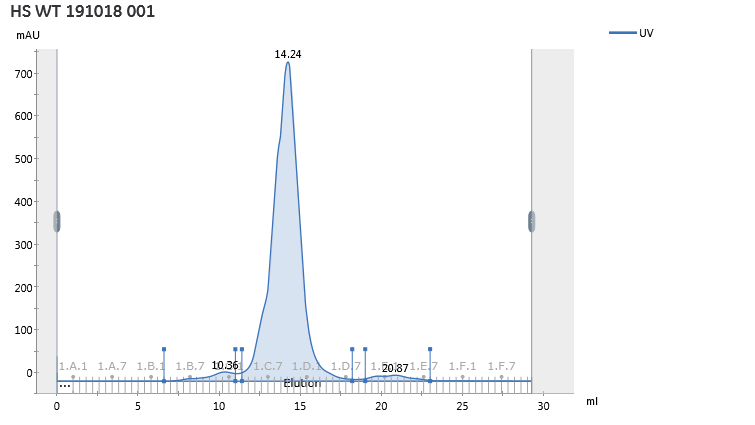
\includegraphics[width=\textwidth]{img/sec_wt}
        \caption{SEC graph of wildtype}
        \label{fig:sec_wt}
    \end{subfigure}
    ~
    \begin{subfigure}{0.45\textwidth}
        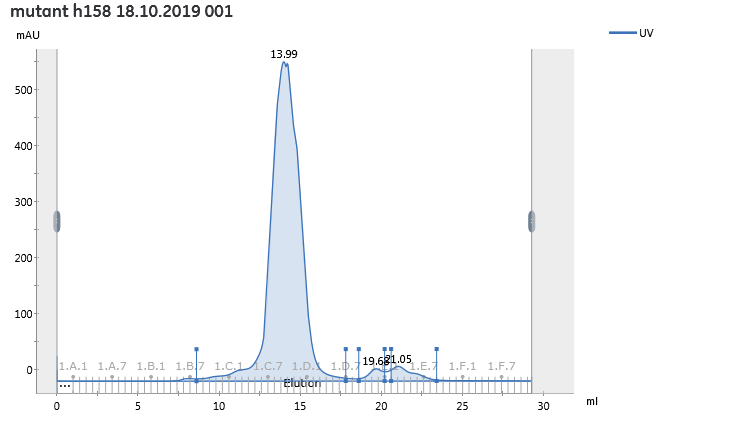
\includegraphics[width=\textwidth]{img/sec_mut}
        \caption{SEC graph of mutant}
        \label{fig:sec_mut}
    \end{subfigure}

    \begin{subfigure}{0.45\textwidth}
        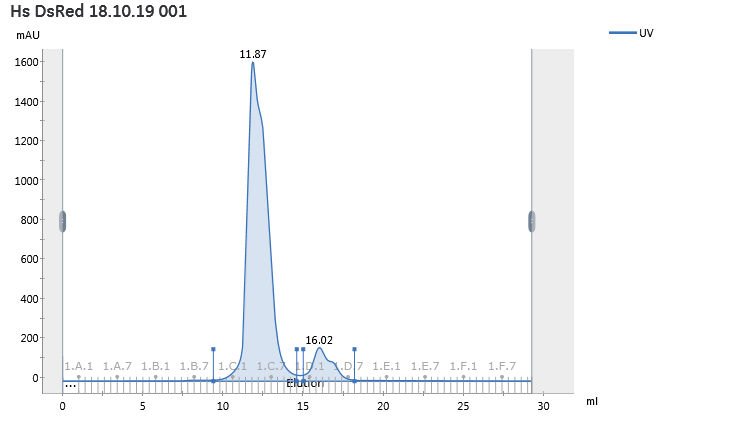
\includegraphics[width=\textwidth]{img/sec_dsred}
        \caption{SEC graph of dsRed}
        \label{fig:sec_dsred}
    \end{subfigure}
    \caption{SEC graphs of three SOO variants}
    \label{fig:sec}
\end{figure}

\section{Protein concentration determination}

Figure \ref{fig:hs_concentration} shows the absorption of the three protein
samples at various wavelengths. The absorption of use to us is the one at
\SI{561}{\nm} which is the absorbance of the two hemes within SOO.

In a first step, the absorption difference at \SI{561}{\nm} between the
oxidated and reduced forms was calculated. In order to compensate the fact that
the baseline of the reduced form was lower, the average absorption difference
in the range of \SIrange{580}{600}{\nm} was calculated, and added to the
previously calculated absorption difference at \SI{561}{\nm}.

Finally, using the path length of the cuvette of \SI{1}{\cm}, the provided
extinction coefficient of \SI{46.36}{\per\milli\Molar\per\cm} and the dilution
factor of \SI{375} the protein concentration was calculated using Beer's law.
These metrics including the final concentration are shown in table
\ref{tbl:hs_concentration}.

\begin{figure}
	\centering
	\includegraphics[width=0.8\textwidth]{img/hs_concentration.png}
	\caption{Absorption of HS for concentration determination}
	\label{fig:hs_concentration}
\end{figure}

\begin{table}
	\centering
	\begin{tabu}{lllll}
		\toprule
		Protein & $\Delta_{\text{Absorption at \SI{561}{\nm}}}$ & Baseline & $\Delta_{\text{Absorption at \SI{561}{\nm} corr}}$ & Concentration [\si{\milli\Molar}] \\
		\midrule
		Wildtype & 0.042 & 0.004 & 0.046 & 0.372 \\
		Mutant & 0.043 & 0.006 & 0.049 & 0.396 \\
		dsRed & 0.068 & 0.013 & 0.081 & 0.655 \\
		\bottomrule
	\end{tabu}
	\caption{Concentration of purified HS}
	\label{tbl:hs_concentration}
\end{table}

\section{SDS PAGE}

The results of the SDS page gels are shown in figure \ref{fig:sds}.

\begin{figure}[h!]
    \centering
    \begin{subfigure}{0.7\textwidth}
        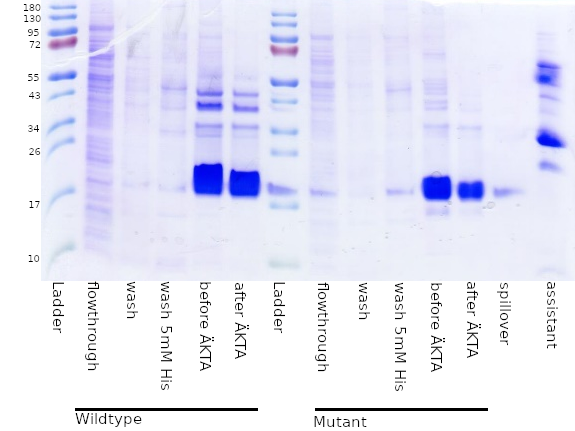
\includegraphics[width=\textwidth]{img/sds_wt_mut}
        \caption{SDS PAGE gel of wildtype and mutant}
        \label{fig:sds_wt_mut}
    \end{subfigure}

    \begin{subfigure}{0.7\textwidth}
        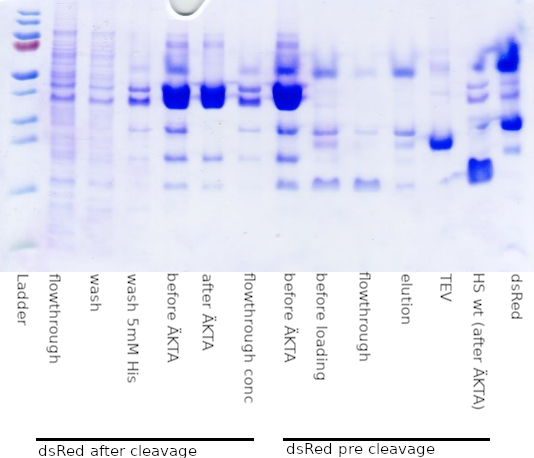
\includegraphics[width=\textwidth]{img/sds_dsred_tev_cleavage.png}
        \caption{SDS PAGE gel of dsRed including cleaved dsRed}
        \label{fig:sds_dsred_cleaved}
    \end{subfigure}
    \caption{SDS gels of three protein variants}
    \label{fig:sds}
\end{figure}

\section{Fluorescence measurements}

The results of the fluorescence measurements for tracking losses during
purification are shown in figure \ref{fig:purification_fluorescence}.
Fluorescence measurements were scaled to the volume the sample had at the time
of the aliquot being stored. This allowed using the so-adjusted fluorescence
value as an indicator of the amount of protein - rather than the concentration
of protein - which were present in the sample at the given stage.

\begin{figure}
	\centering
	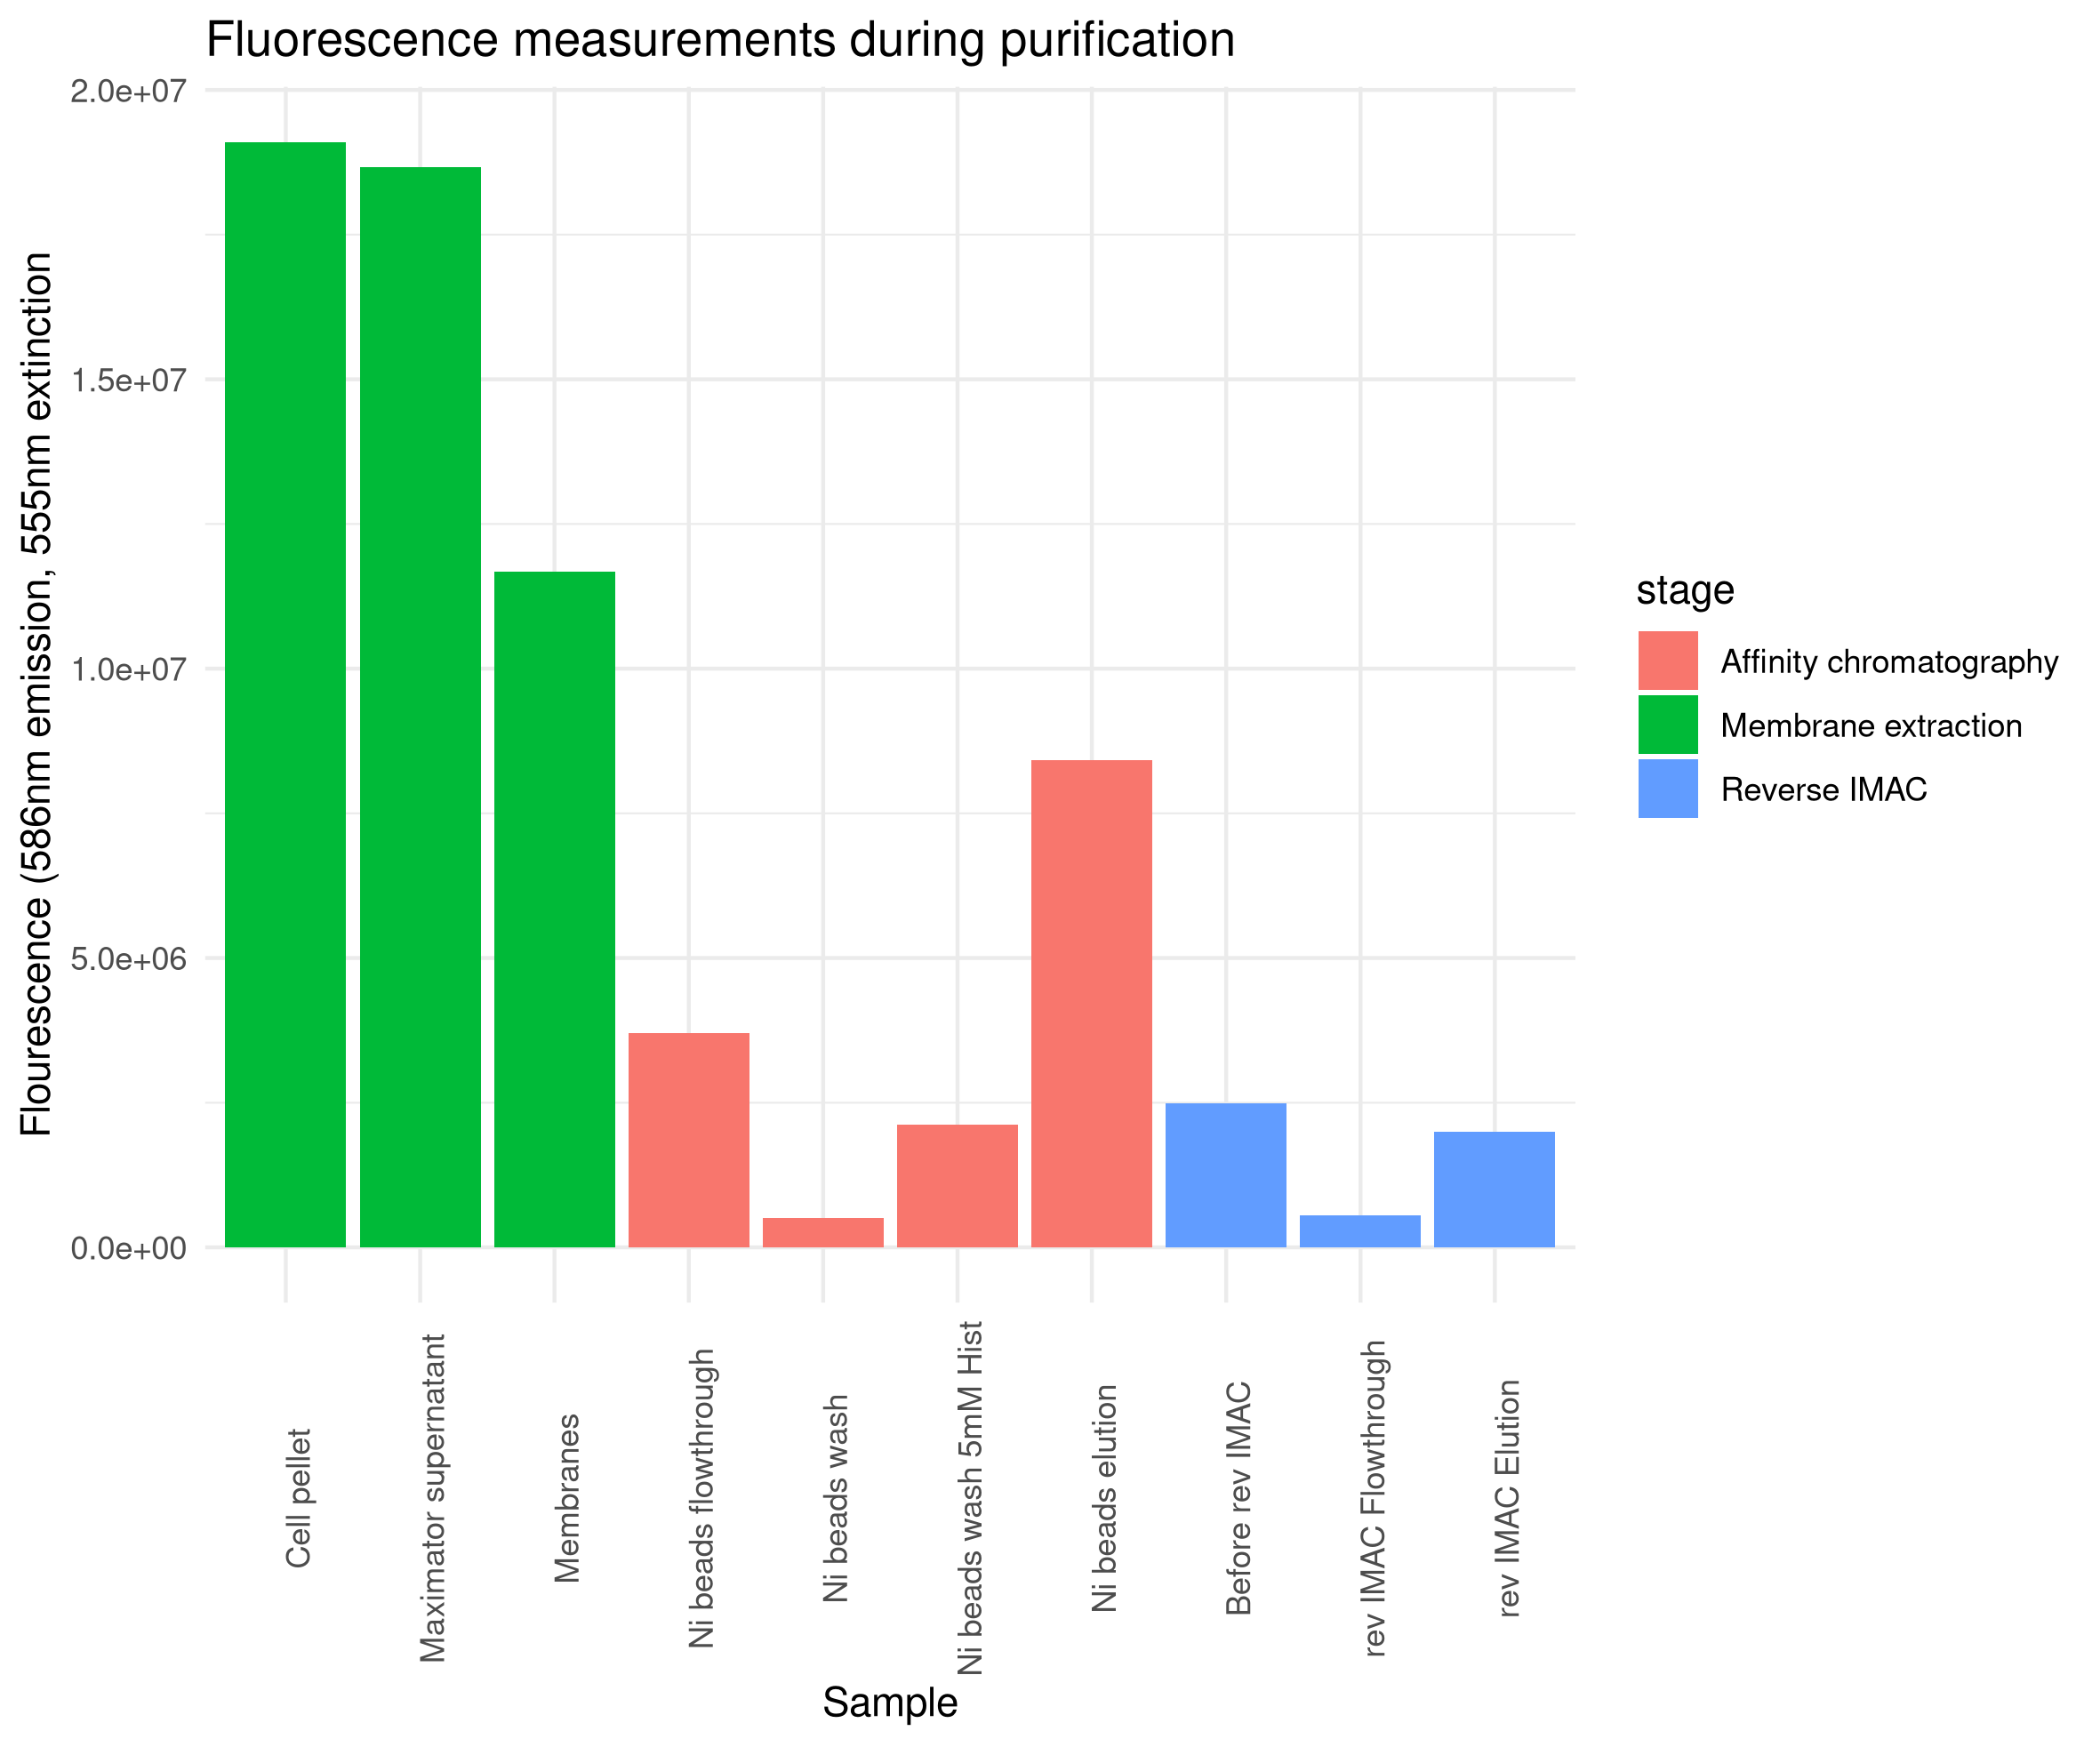
\includegraphics[width=0.8\textwidth]{img/purification_fluorescence.png}
	\caption{Fluorescence measurements to track purification losses}
	\label{fig:purification_fluorescence}
\end{figure}

\section{Relative enzyme reduction}

\subsection{Quinone}

The absorption measurements of the wildtype, mutant and control to follow the
reduction of HS are shown in figure \ref{fig:reduction_quinol}.

To determine the relative reduction of HS by quinol, three absorption values
were considered. The average absorption value between \SIrange{0.8}{0.9}{\min}
was used as a baseline, which was subtracted from the other two measurements.
The average absorption between \SIrange{2.5}{2.6}{\min} allowed following the
reduction of HS by quinol, while the average absorption between
\SIrange{3.9}{4}{\min} gave the absorption value where all HS had been reduced
by DTT. These three values, as well as the resulting relative reduction of HS
by quinol, are shown in table \ref{tbl:reduction_quinol}.

\begin{figure}
	\centering
	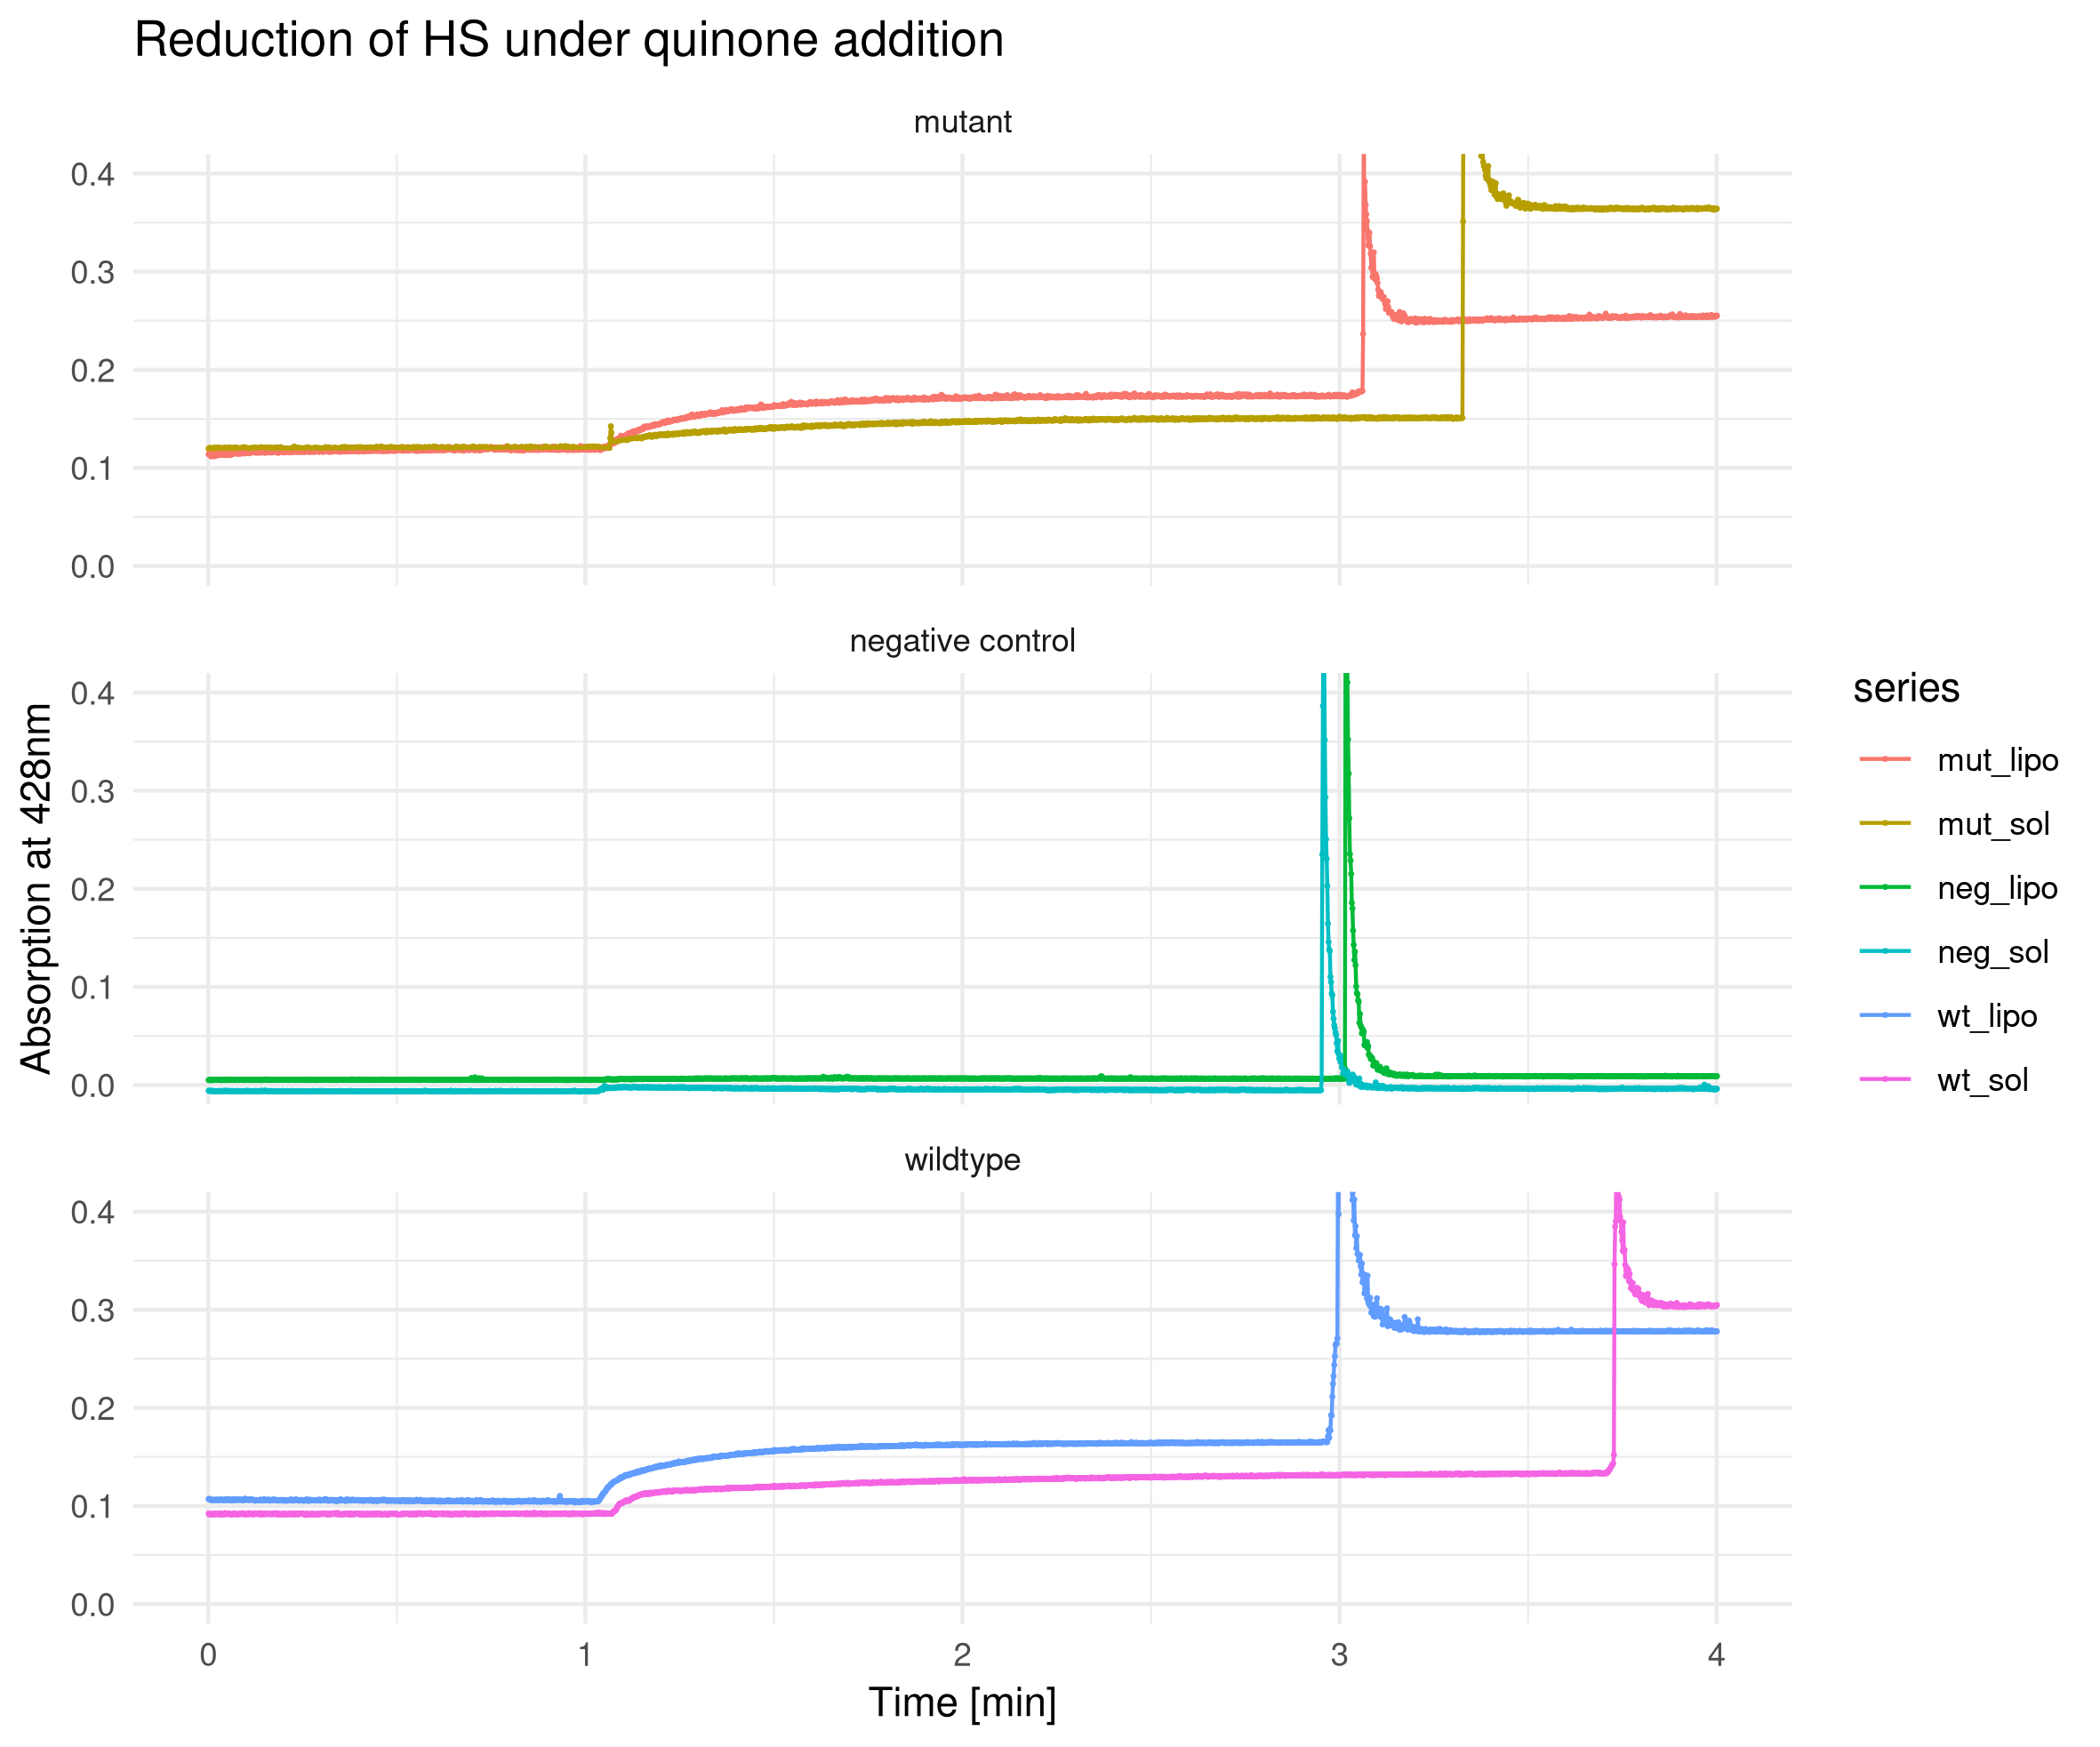
\includegraphics[width=0.8\textwidth]{img/reduction_quinol.png}
	\caption{Absorbance of HS to track reduction due to quinol}
	\label{fig:reduction_quinol}
\end{figure}


\begin{table}
	\centering
	\begin{tabu}{llllll}
		\toprule
		Protein & State & Baseline & Absorption Quinol & Absorption \SI{100}{\percent} & Rel reduction \\
		\midrule
		Wildtype & Liposomes & 0.105 & 0.164 & 0.278 & \SI{34}{\percent} \\
		Wildtype & Solubilized & 0.092 & 0.130 & 0.304 & \SI{18}{\percent} \\
		Mutant & Liposomes & 0.119 & 0.173 & 0.254 & \SI{40}{\percent} \\
		Mutant & Solubilized & 0.121 & 0.150 & 0.364 & \SI{12}{\percent} \\
		\bottomrule
	\end{tabu}
	\caption{Relative reduction of HS by quinol addition}
	\label{tbl:reduction_quinol}
\end{table}

\subsection{Superoxide}

The corresponding graphs and tables for the reduction of HS in presence of
superoxide are shown in figure \ref{fig:reduction_superox} and table
\ref{tbl:reduction_superox}.

\begin{figure}
	\centering
	\includegraphics[width=0.9\textwidth]{img/reduction_superox.png}
	\caption{Absorbance of HS to track reduction due to superoxide}
	\label{fig:reduction_superox}
\end{figure}

\begin{table}
	\centering
	\begin{tabu}{lllllll}
		\toprule
		Protein & State & SOD & Baseline & Abs Superox & Abs \SI{100}{\percent} & Rel reduction \\
		\midrule
		Mutant   & Liposomes   & No   &          0.0854    &            0.103               &   0.218         &  \SI{14}{\percent}   \\
		Mutant   & Liposomes   & Yes  &            0.0815  &              0.0828            &     0.202       &  \SI{01}{\percent}  \\
		Mutant   & Solubilized & No   &          0.0650    &            0.118               &   0.251         &  \SI{28}{\percent}   \\
		Mutant   & Solubilized & Yes  &            0.0862  &              0.0892            &     0.276       &  \SI{02}{\percent}  \\
		Wildtype & Liposomes   & No   &          0.103     &            0.126               &   0.279         &  \SI{13}{\percent}  \\
		Wildtype & Liposomes   & Yes  &            0.0820  &              0.0846            &     0.272       &  \SI{1 }{\percent} \\
		Wildtype & Solubilized & No   &          0.0874    &            0.143               &   0.277         &  \SI{29}{\percent}  \\
		Wildtype & Solubilized & Yes  &            0.0980  &              0.0985            &     0.280       &  \SI{0 }{\percent} \\
		\bottomrule
	\end{tabu}
	\caption{Relative reduction of HS by superox addition}
	\label{tbl:reduction_superox}
\end{table}

\subsection{Relative reduction}

The relative reductions by both, superoxide and quinol, are shown in figure
\ref{fig:reduction_relative}.

\begin{figure}
    \centering
    \begin{subfigure}{0.45\textwidth}
	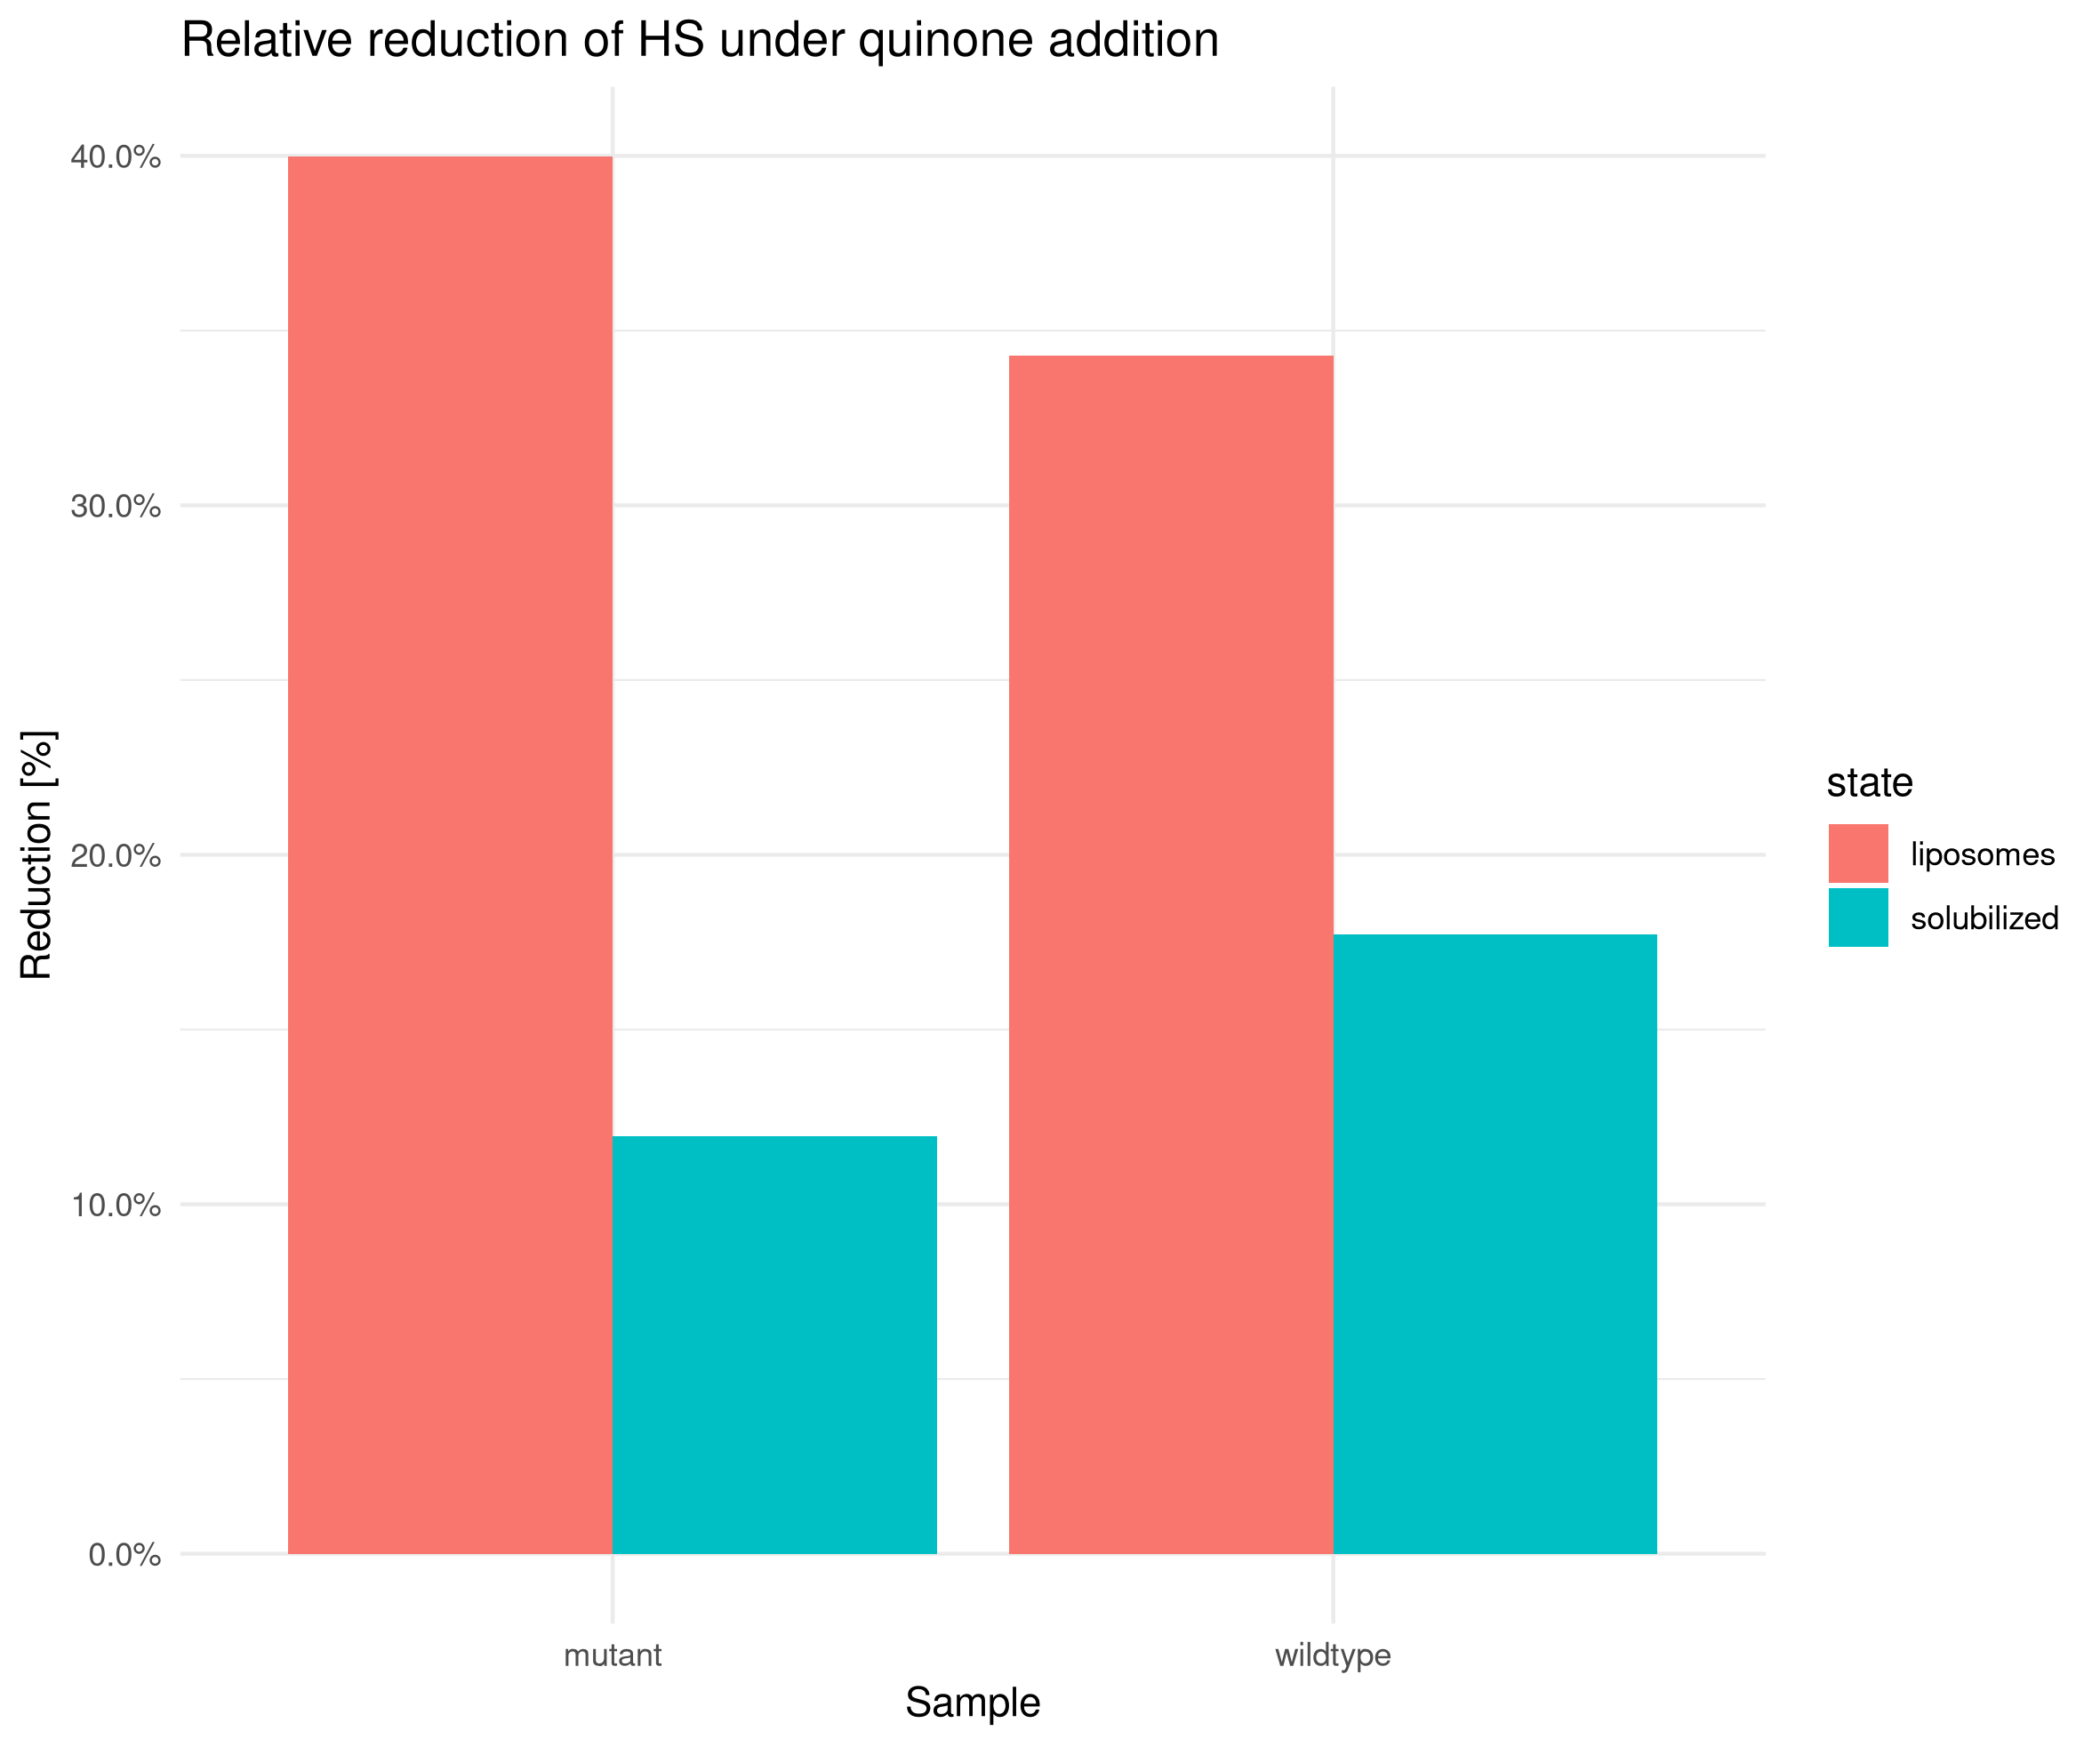
\includegraphics[width=\textwidth]{img/reduction_quinol_relative.png}
	\caption{Relative reduction of HS by quinol}
	\label{fig:reduction_quinol_relative}
    \end{subfigure}
    ~
    \begin{subfigure}{0.45\textwidth}
	\centering
	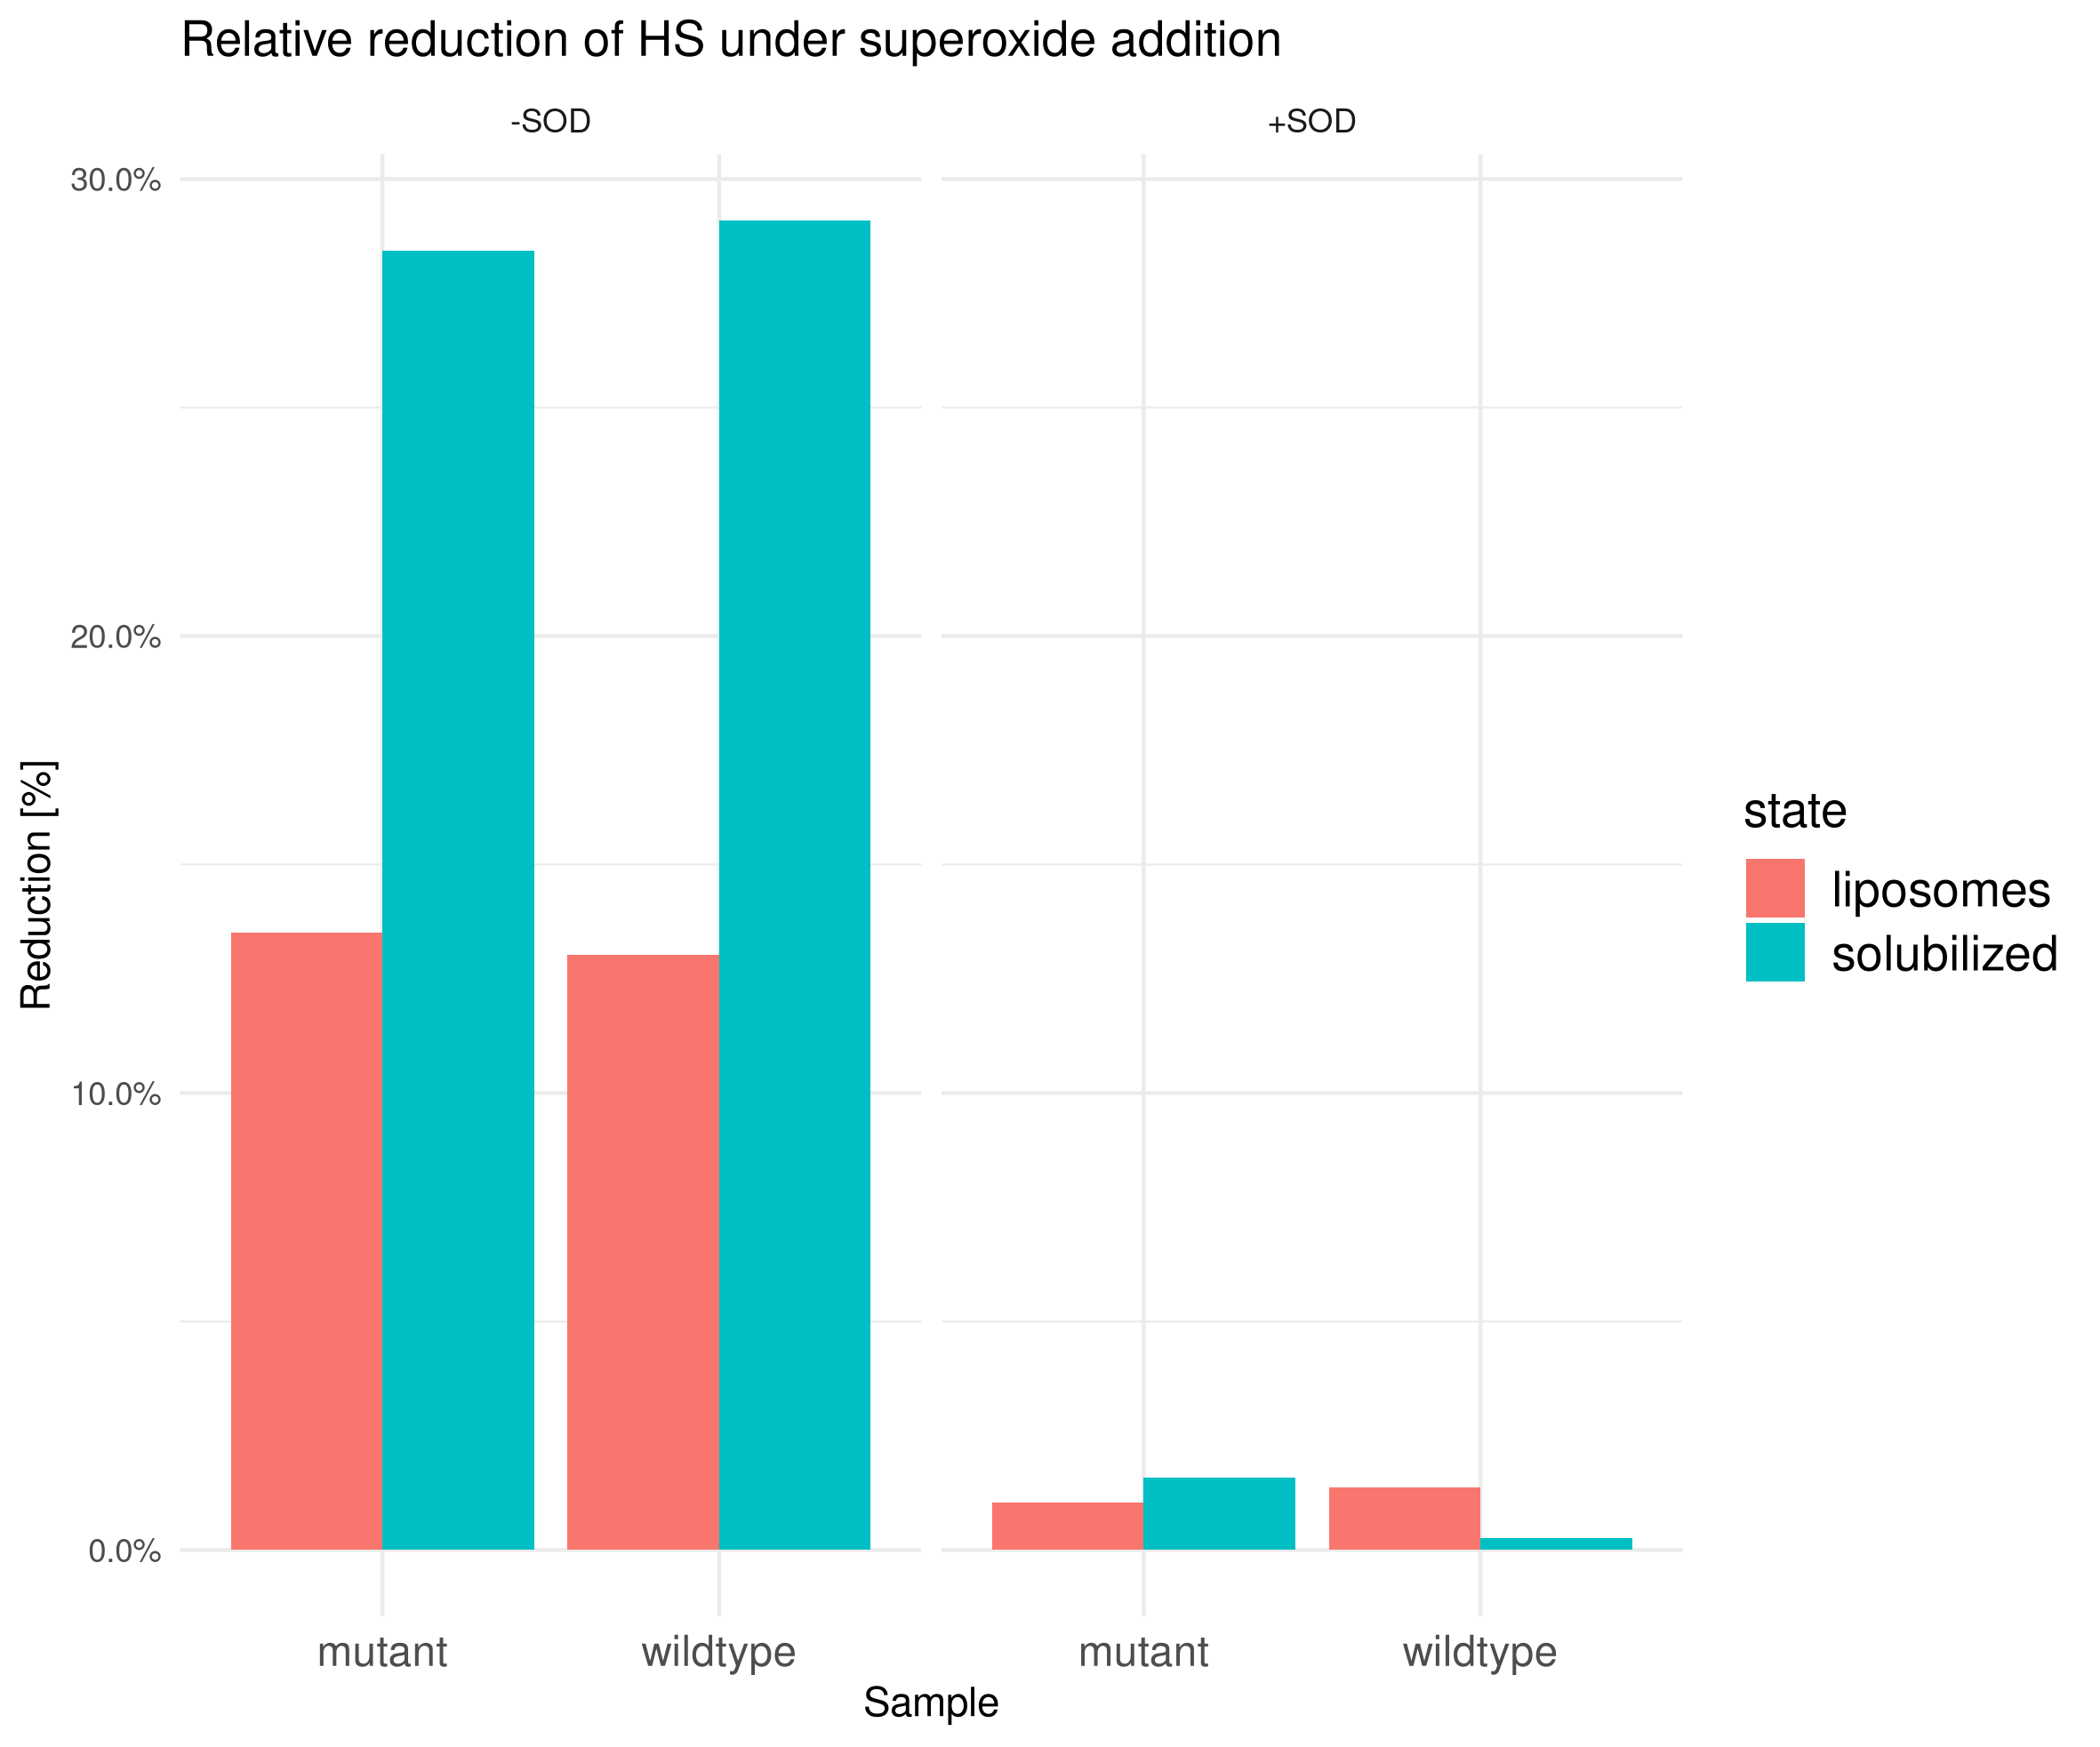
\includegraphics[width=\textwidth]{img/reduction_superox_relative.png}
	\caption{Relative reduction of HS by superox}
	\label{fig:reduction_superox_relative}
    \end{subfigure}
    \caption{Relative reduction of HS by quinol and superoxide}
    \label{fig:reduction_relative}
\end{figure}

\section{Fluorescence measurements before and after cleavage}

The results of the various fluorescence measurements of cleaved and uncleaved
HS-dsRed including the quenching with copper are shown in figure
\ref{fig:dsred_cleavage_fluorescence}.

\begin{figure}
	\centering
	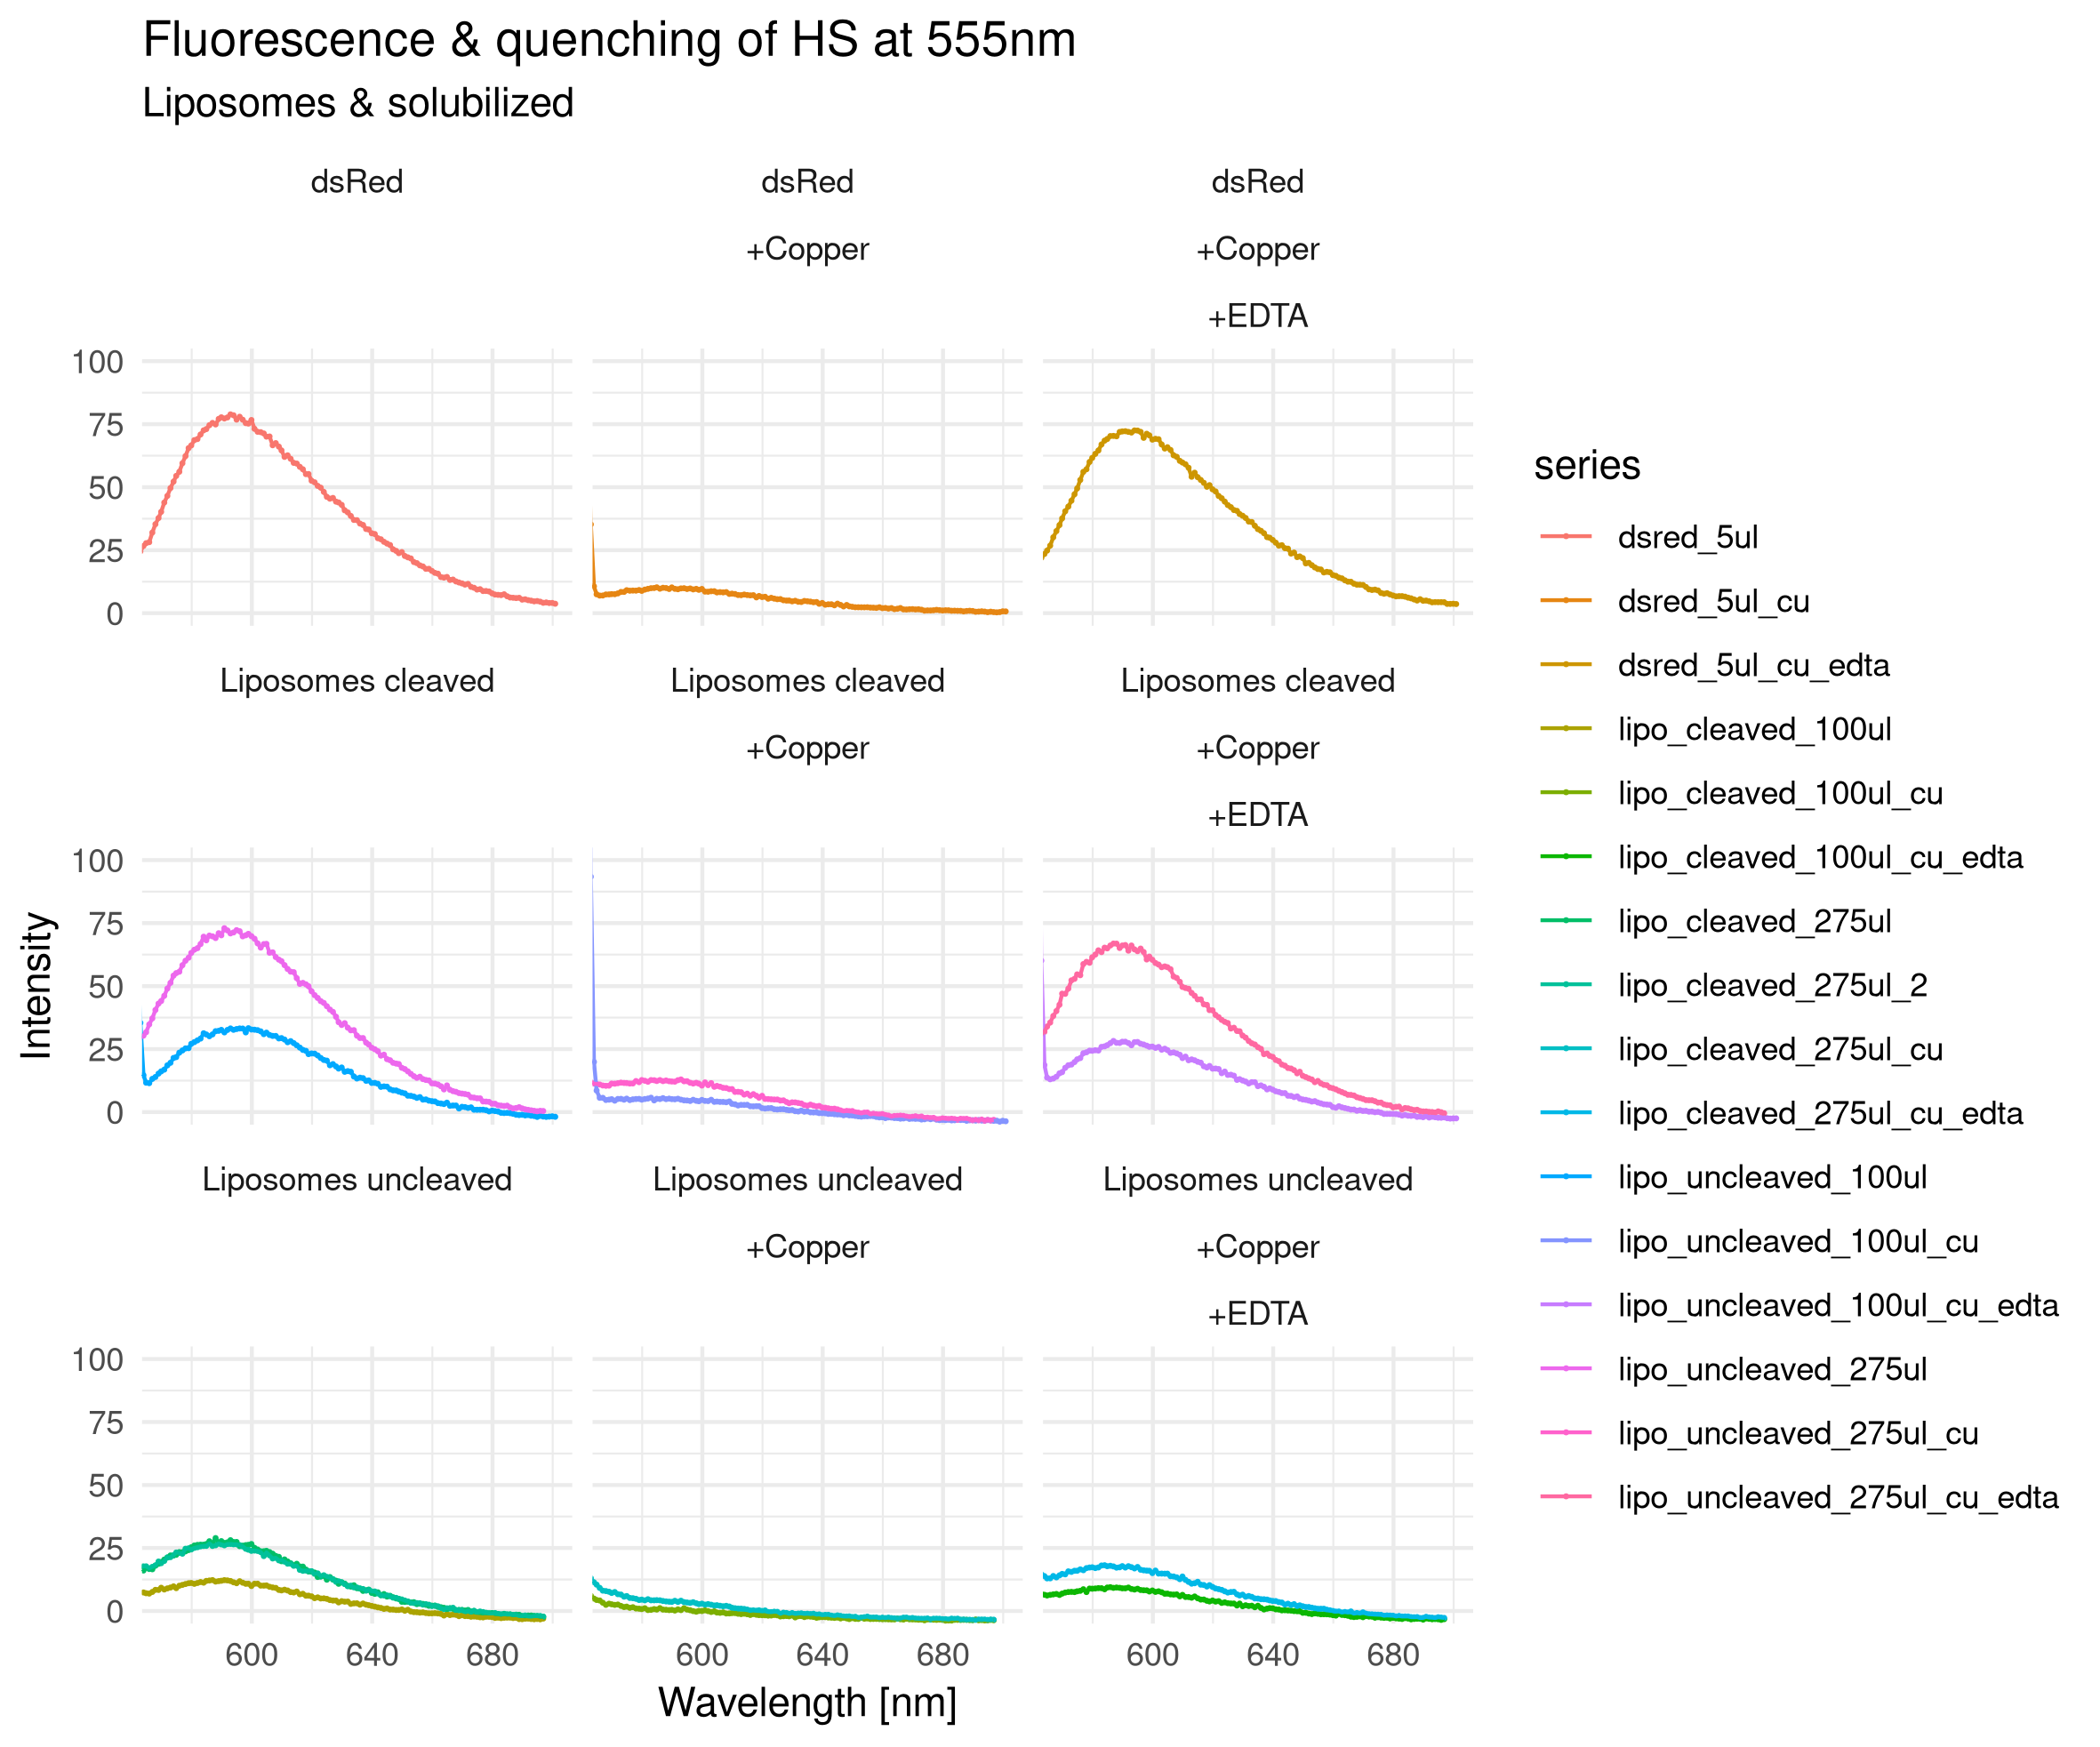
\includegraphics[width=\textwidth]{img/dsred_cleavage_fluorescence.png}
	\caption{Fluorescence and quenching thereof of cleaved and uncleaved dsRed}
	\label{fig:dsred_cleavage_fluorescence}
\end{figure}

\section{Activity measurement}

\subsection{Determining sufficient HS concentrations}

Figures \ref{fig:activity_mut_hs} and \ref{fig:activity_wt_hs} show the
absorption graphs which were used to determine HS concentrations which were
able to quench the reduction of the dye as well as SOD. For the mutant this
turned out to be a volume of \SI{9}{\ul} per cuvette, for the wild type a
volume of \SI{1}{\ul}.

\subsection{Determining $K_m$}

Figure \ref{fig:activity_quinone} shows the absorption graphs when quinone
concentration was gradually lowered. For each of the samples the slope after
enzyme addition was determined. As a baseline the slope of the SOD sample after
SOD addition was determined, as well as the average of all slopes after XO
addition.

This allowed calculating the relative oxidation of superoxide as follows. Let
$s_{\text{xo}}$ be the average slope after XO addition. Let $s_{\text{SOD}}$ be
the slope after SOD addition. Let $s_{\text{sample}}$ be the slope of one
sample after addition of enzyme. The relative oxidation of superoxide of that
one sample is then given as:

\[
	\text{oxidation}_{\text{Superoxide}} = 1 - \frac{s_{\text{sample}}}{s_{\text{XO}} - s_{\text{SOD}}}
\]

These relative oxidation values are shown in figure \ref{fig:activity_km}, as
well as in a LB plot in figure \ref{fig:activity_km_lb}. A linear regression
was performed on the values, which then allowed to calculate the following
$K_m$ values in table \ref{tbl:activity_km}.

\begin{table}
	\centering
	\begin{tabu}{lllll}
		\toprule
		Protein & LB slope $a$ & LB y-intercept $b$ & $v_{\text{max}} = b^{-1}$ & $K_m = v_{\text{max}} \cdot a$ \\
		\midrule
		Wildtype & 0.0065 & 1.1 & \SI{90.9}{\percent} & \SI{0.0059}{\micro\Molar} \\
		Mutant & 0.24 & 1.1 & \SI{90.9}{\percent} & \SI{0.218}{\micro\Molar} \\
		\bottomrule
	\end{tabu}
	\caption{Determination of $K_m$ for HS}
	\label{tbl:activity_km}
\end{table}


\begin{figure}
    \centering
    \begin{subfigure}{0.75\textwidth}
	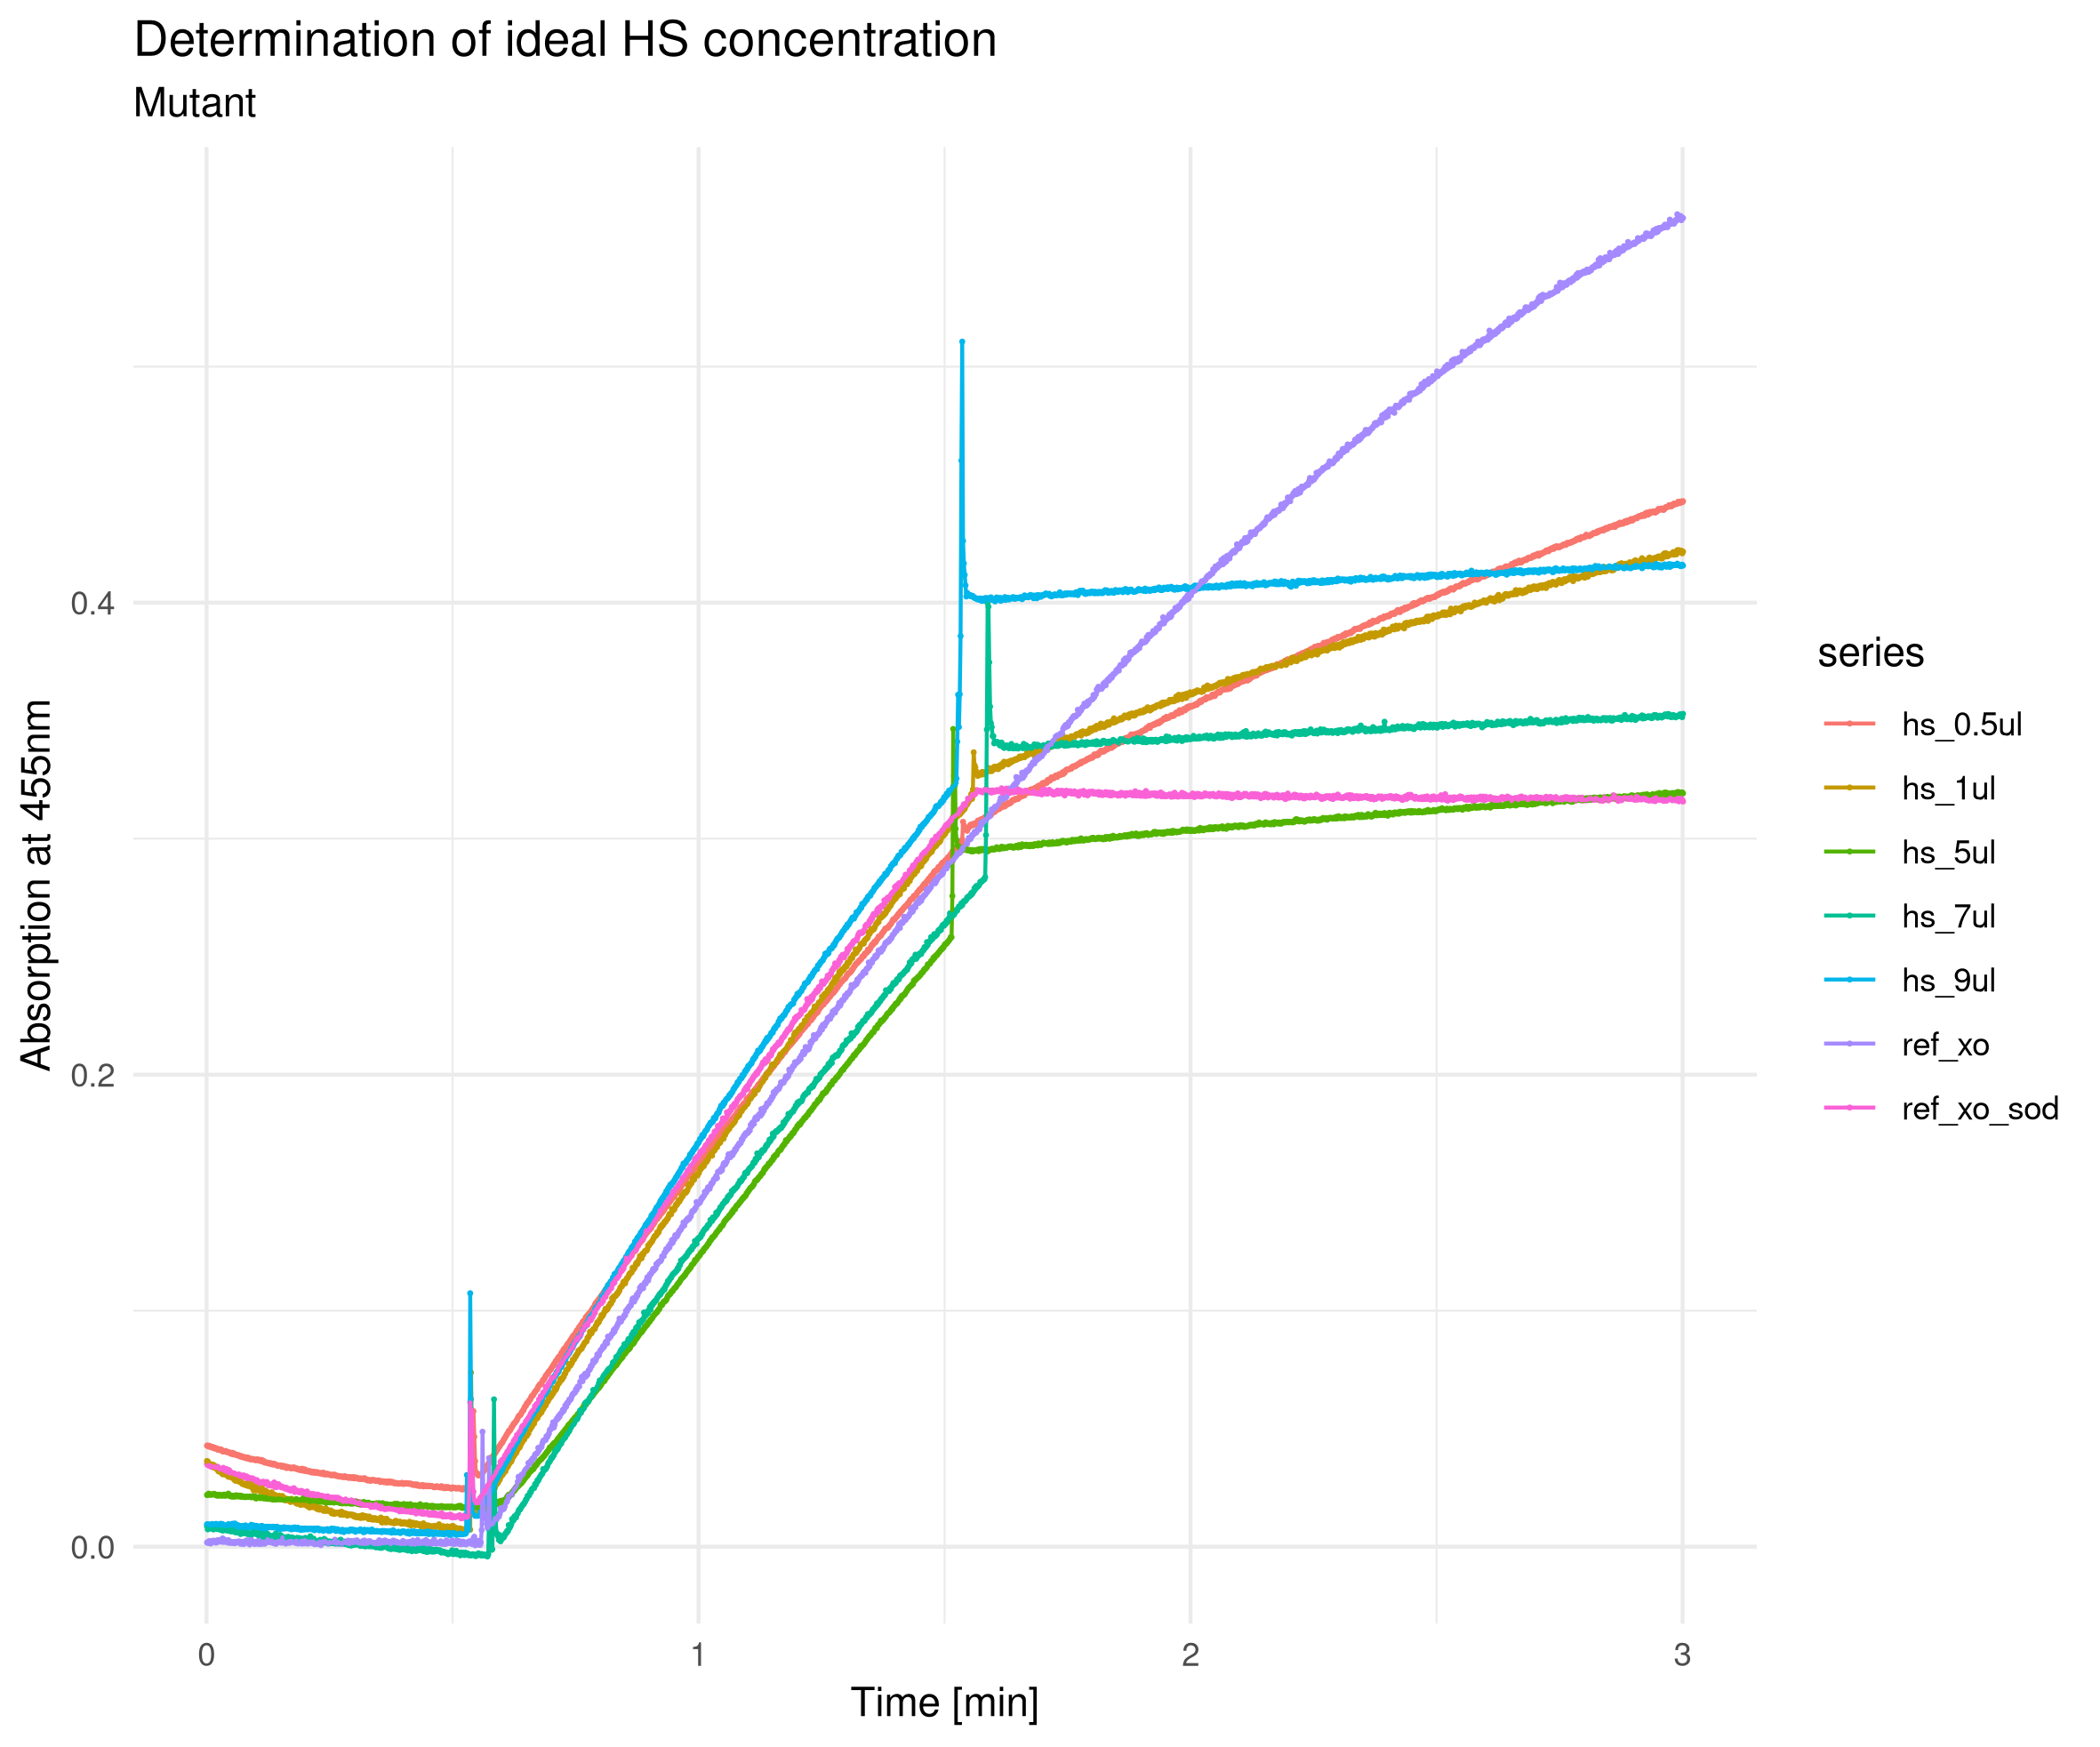
\includegraphics[width=\textwidth]{img/activity_mut_hs.png}
	\caption{HS mutant}
	\label{fig:activity_mut_hs}
    \end{subfigure}

    \begin{subfigure}{0.75\textwidth}
	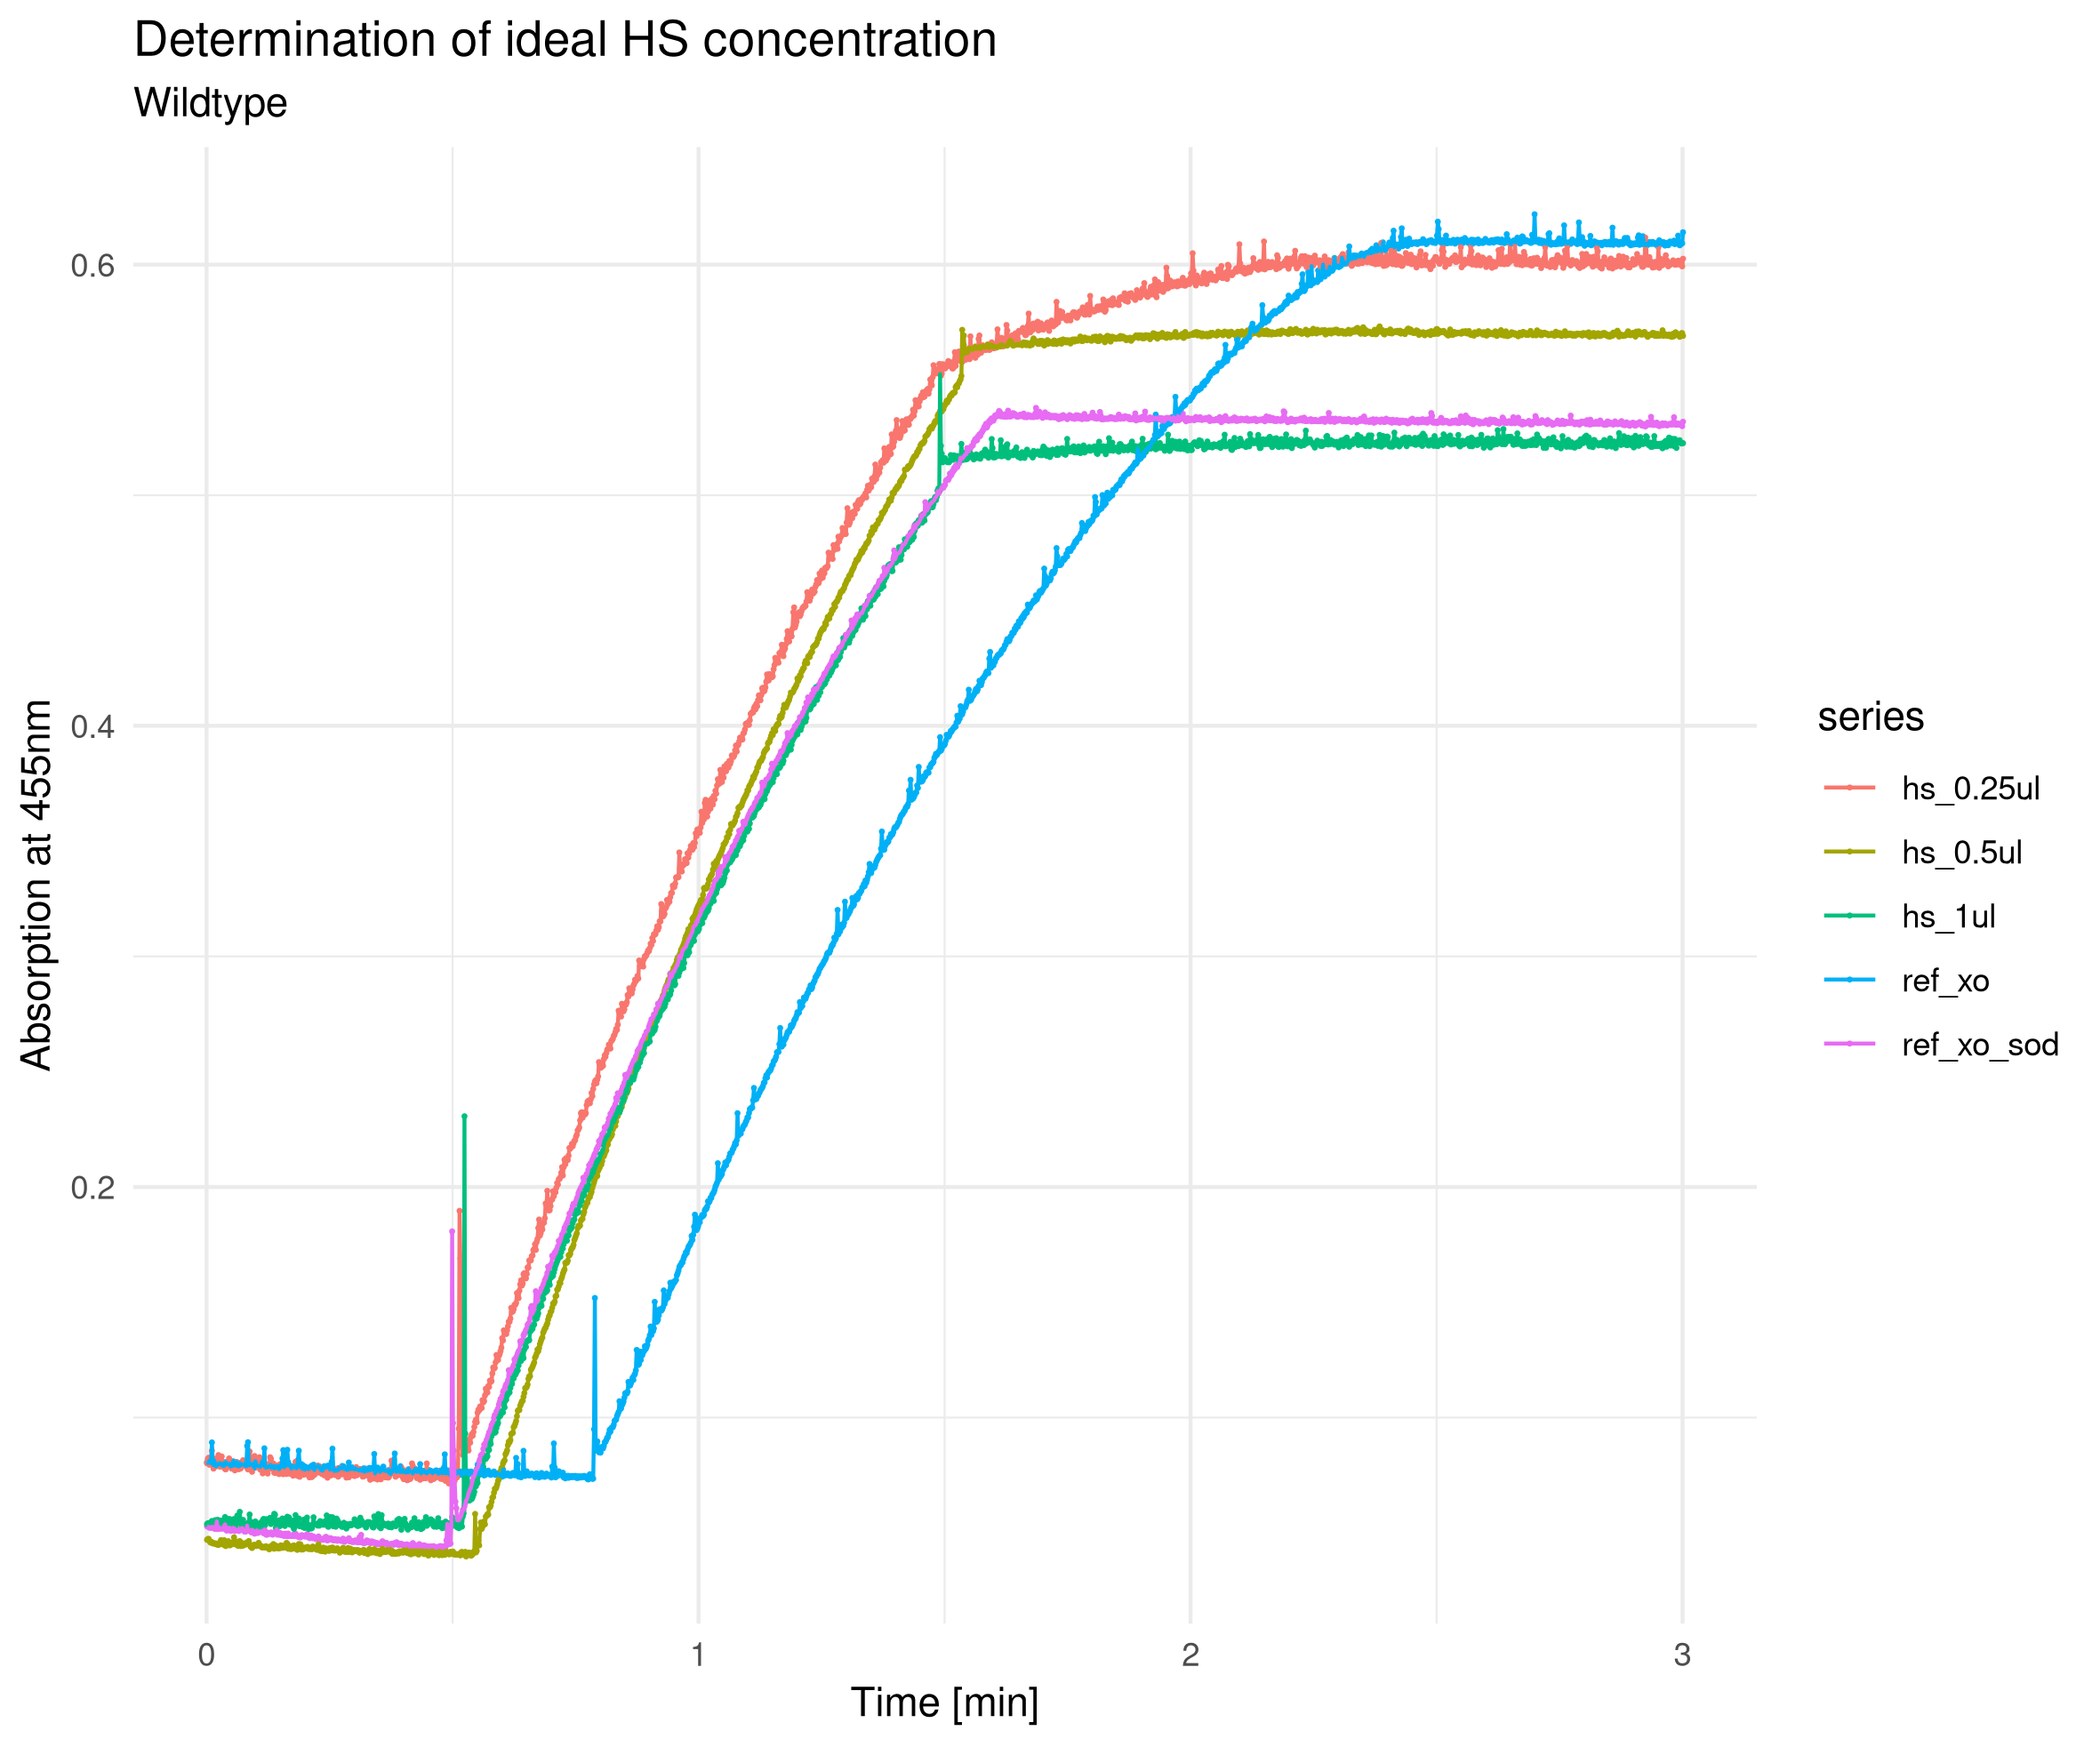
\includegraphics[width=\textwidth]{img/activity_wt_hs.png}
	\caption{HS wildtype}
	\label{fig:activity_wt_hs}
    \end{subfigure}
    \caption{Determination of sufficient HS concentration}
    \label{fig:activity_hs}
\end{figure}

\begin{figure}
    \centering
    \begin{subfigure}{0.75\textwidth}
	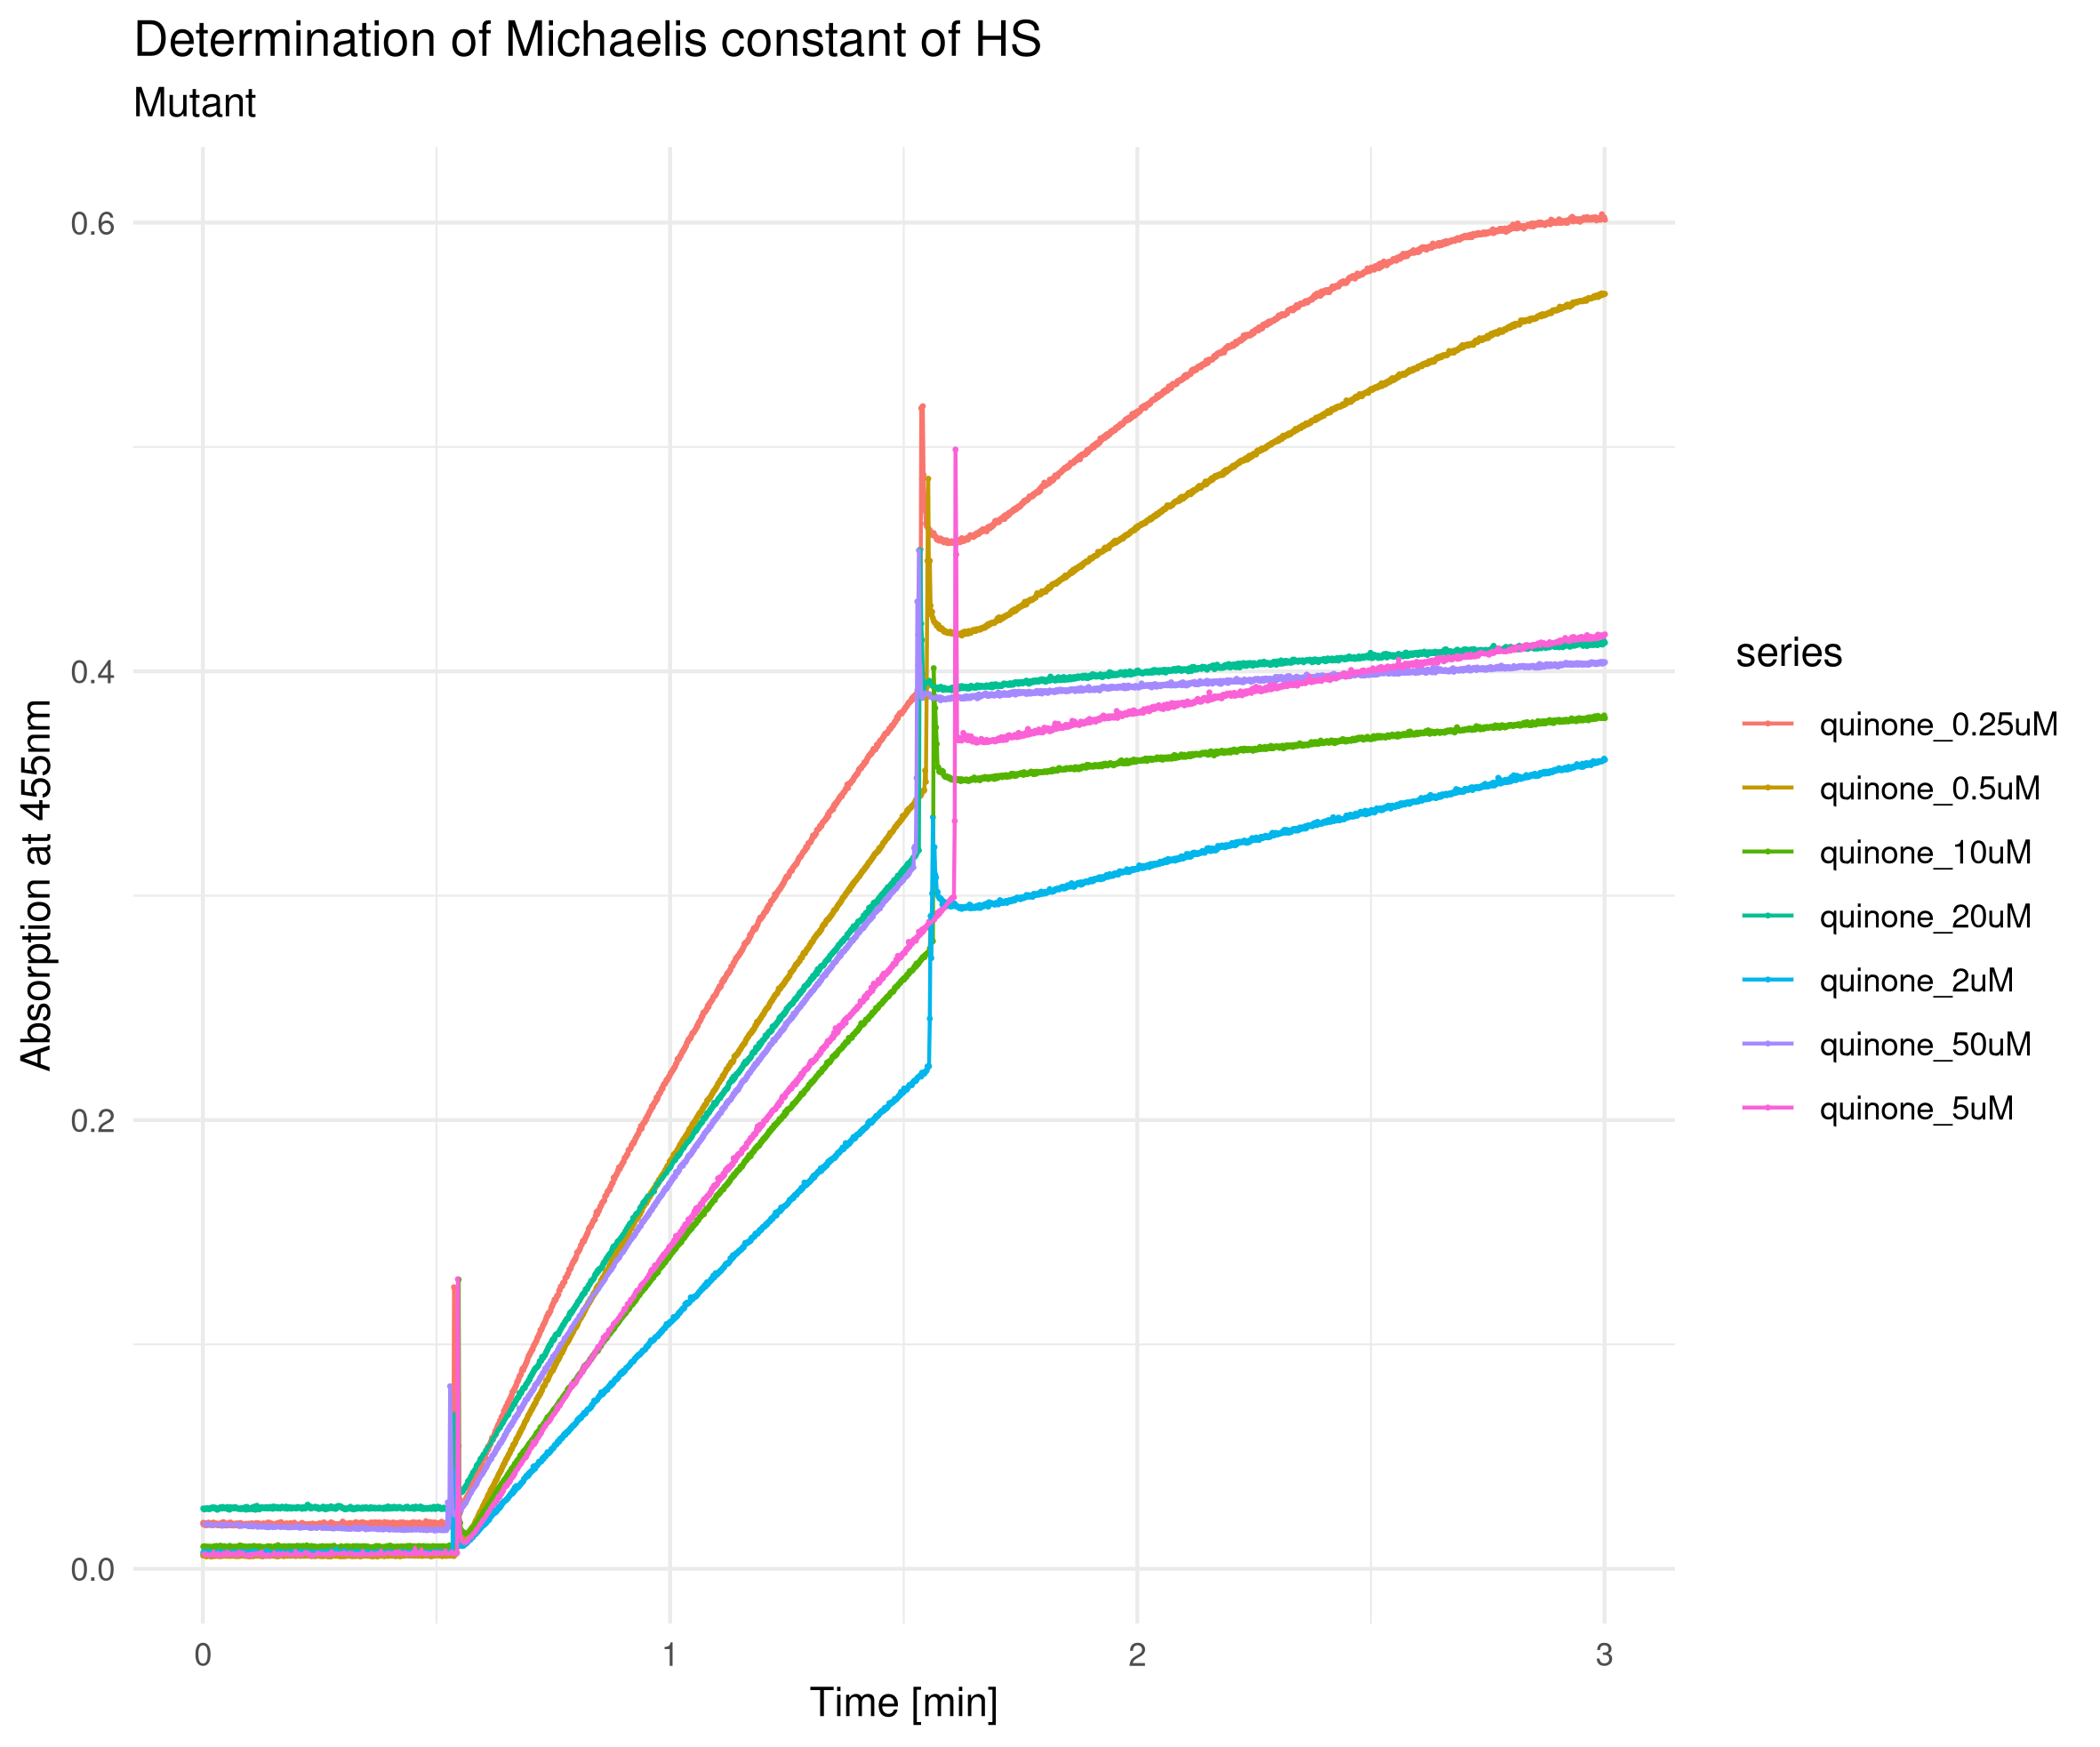
\includegraphics[width=\textwidth]{img/activity_mut_quinone.png}
	\caption{HS mutant}
	\label{fig:activity_mut_quinone}
    \end{subfigure}

    \begin{subfigure}{0.75\textwidth}
	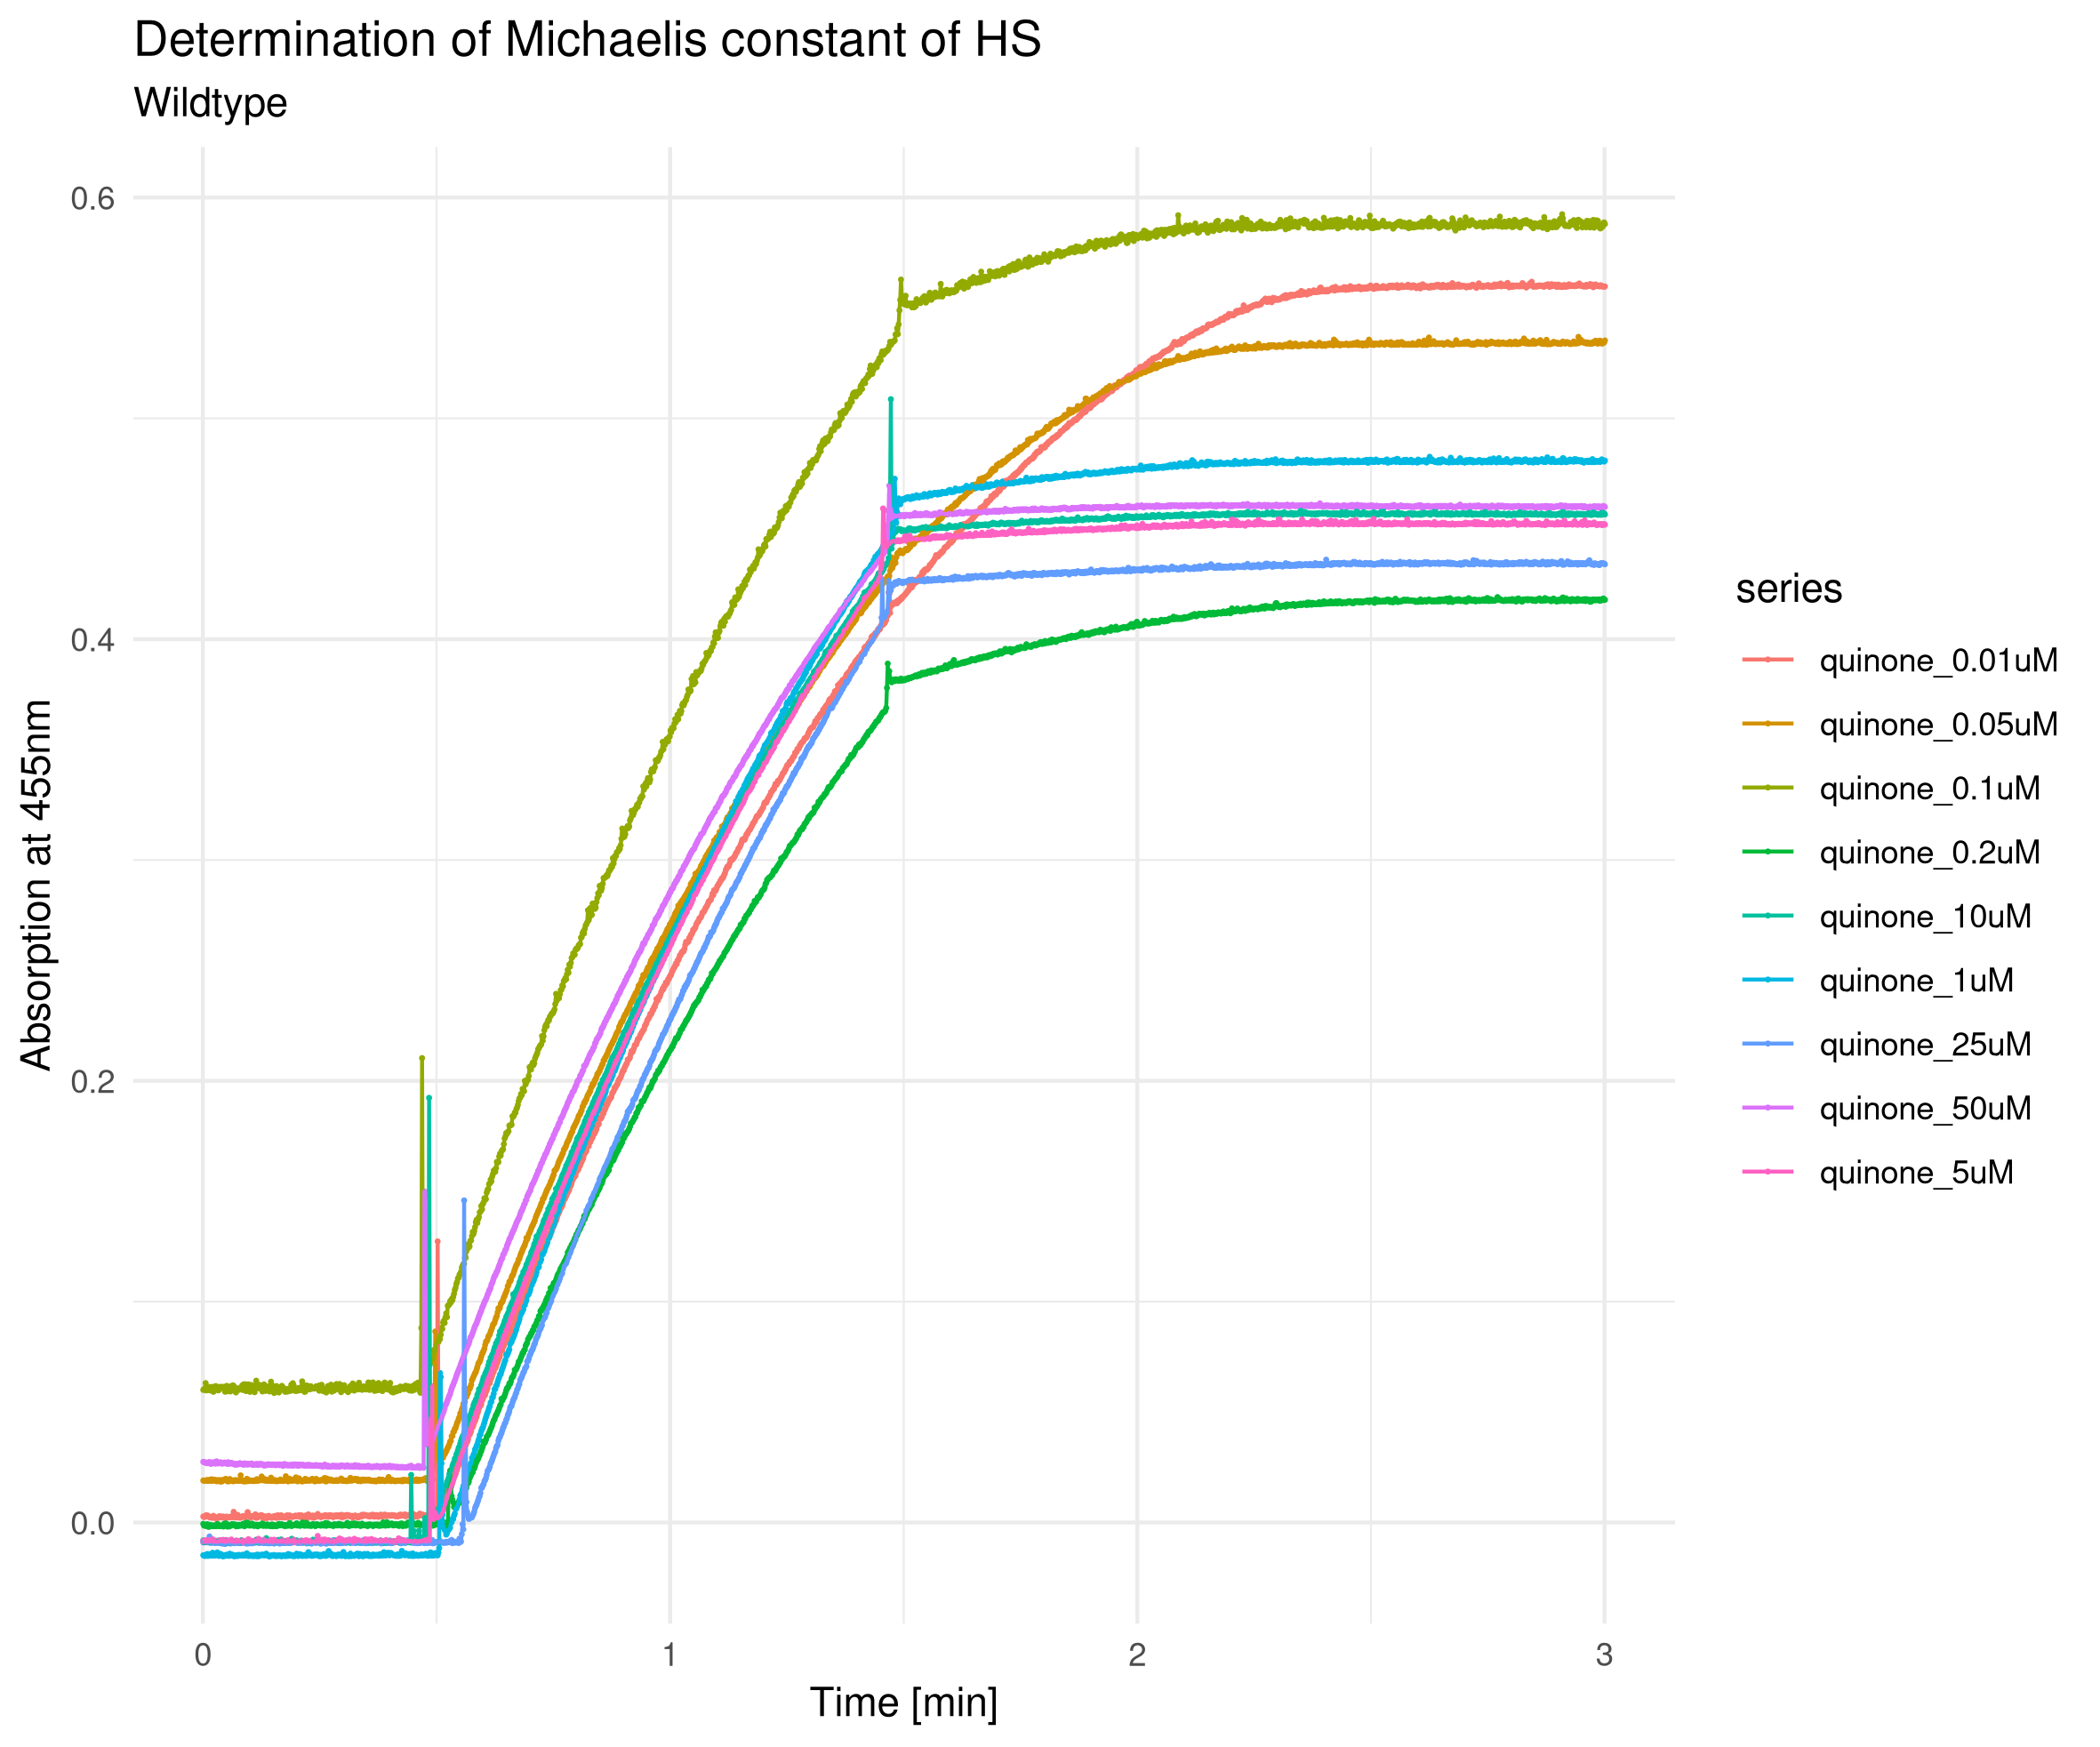
\includegraphics[width=\textwidth]{img/activity_wt_quinone.png}
	\caption{HS wildtype}
	\label{fig:activity_wt_quinone}
    \end{subfigure}
    \caption{Determination of activity depending on Quinone concentration}
    \label{fig:activity_quinone}
\end{figure}

\begin{figure}
    \centering
    \begin{subfigure}{0.45\textwidth}
	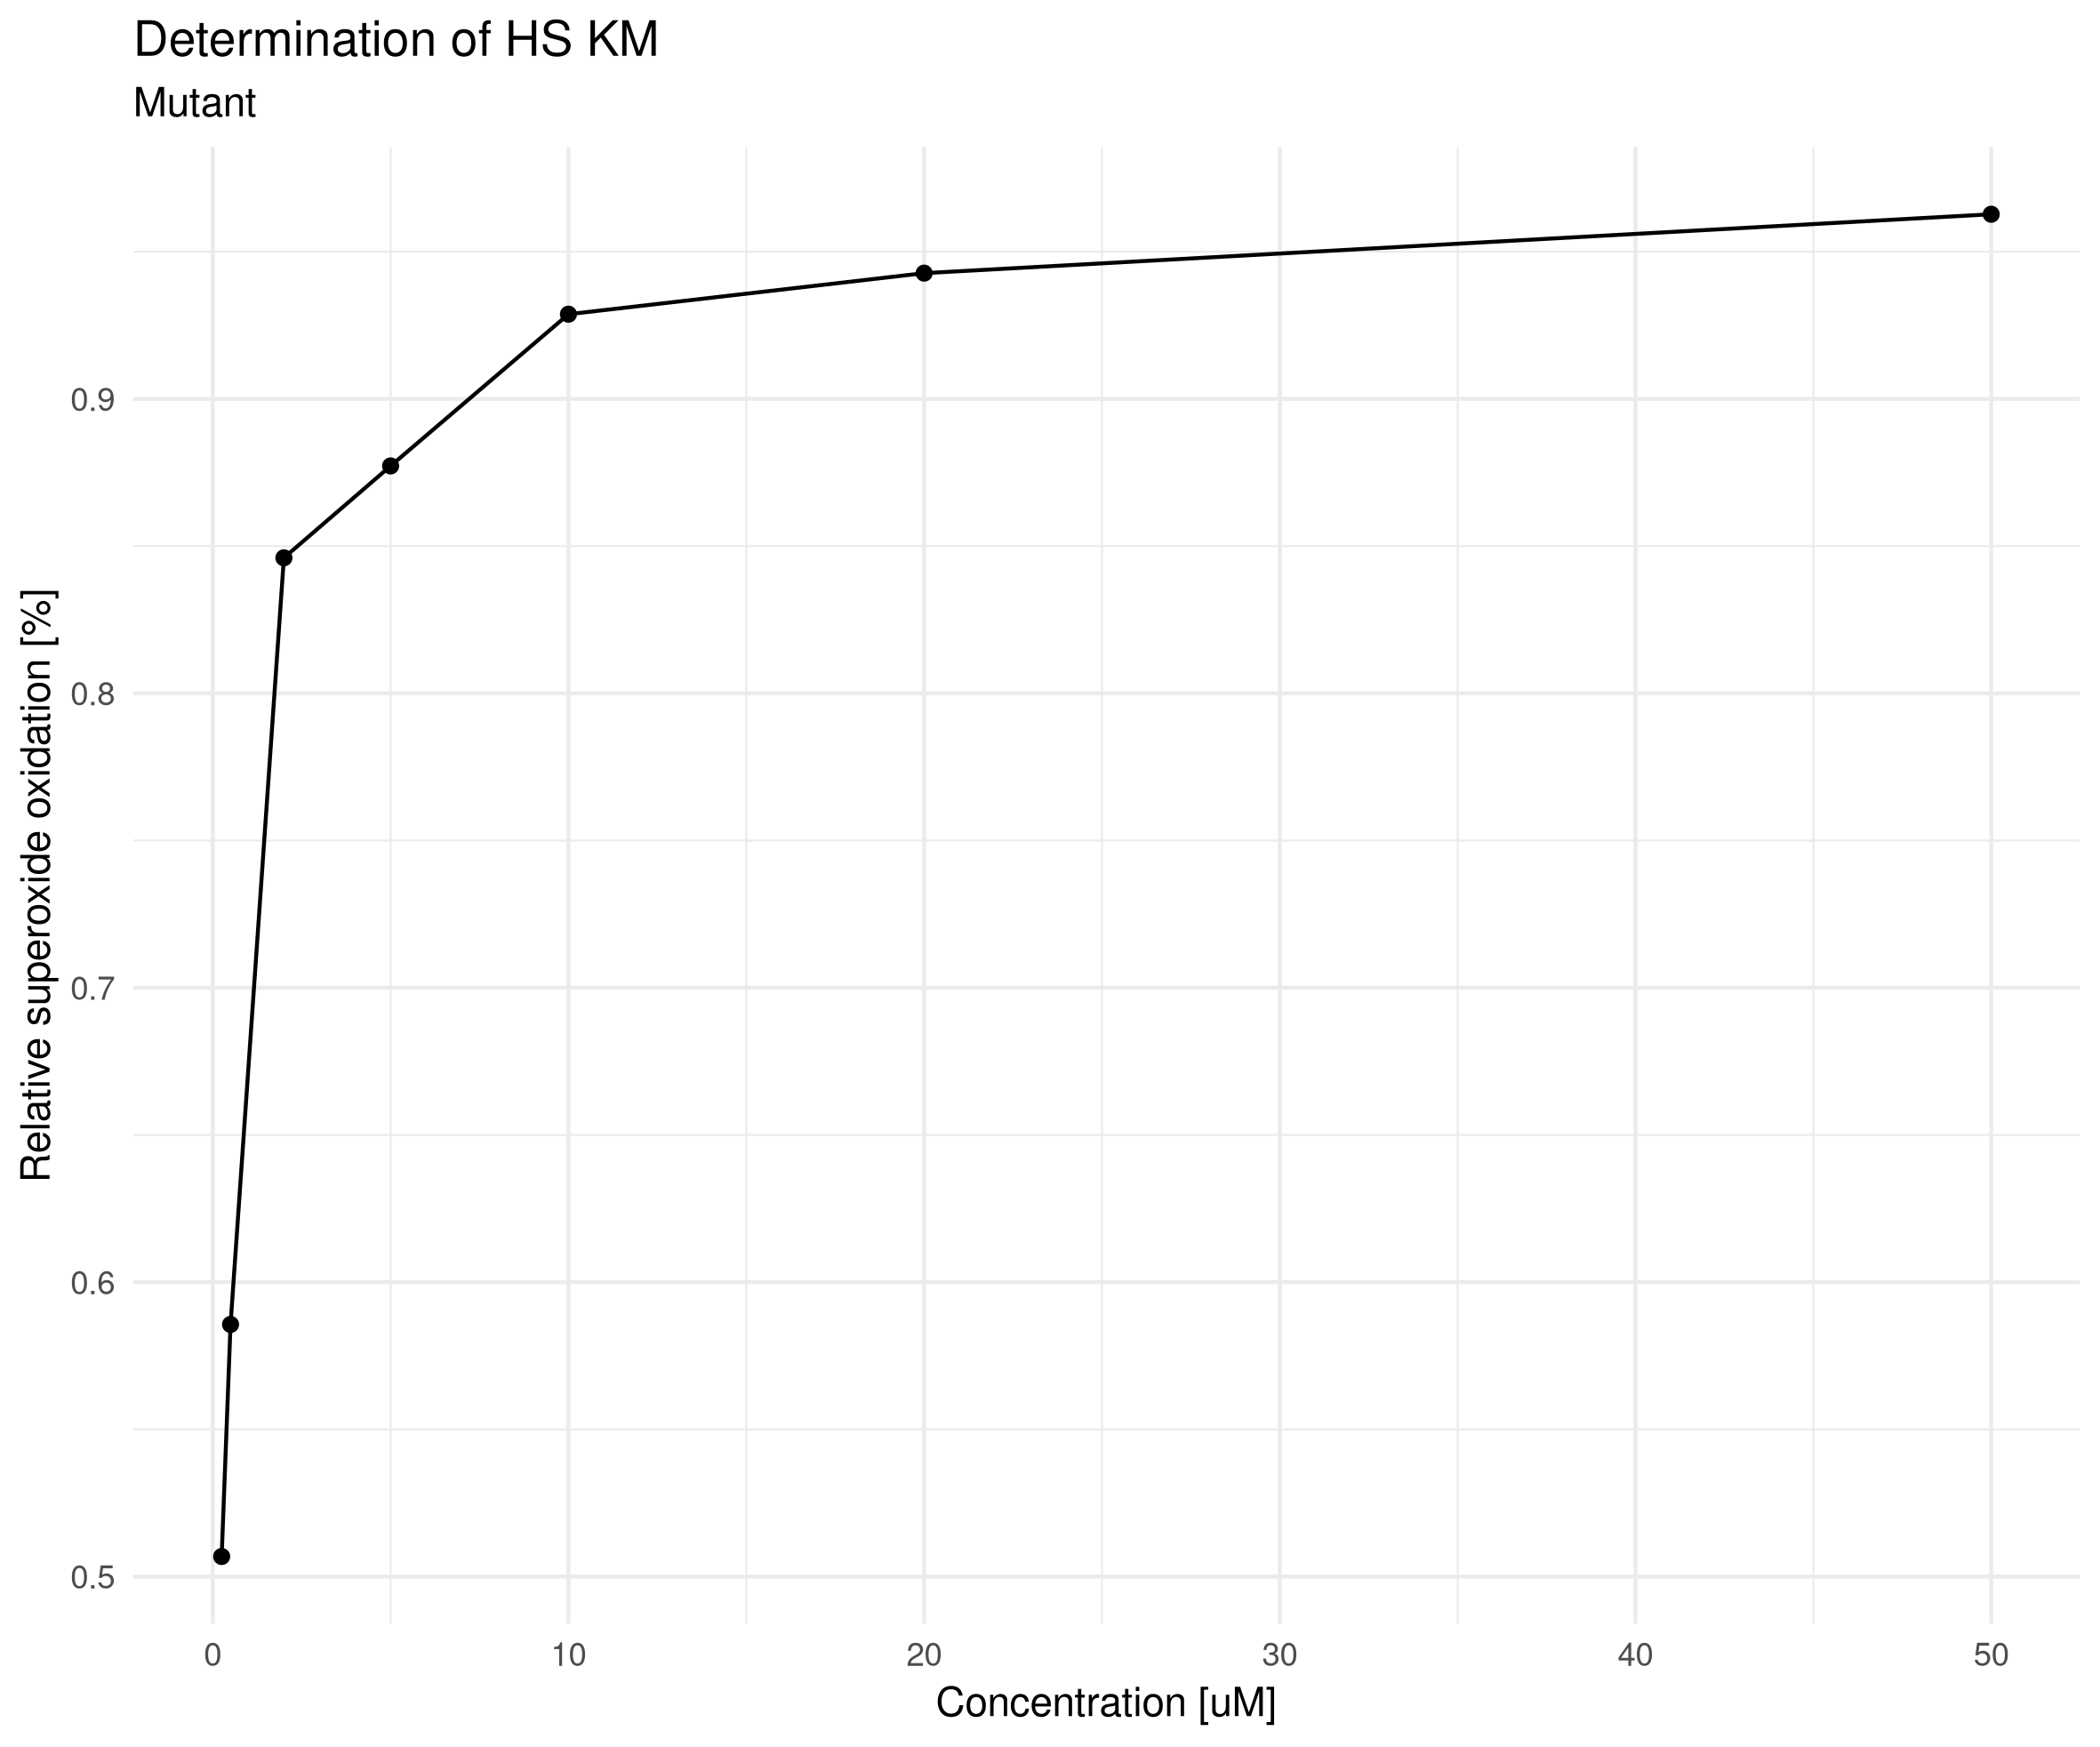
\includegraphics[width=\textwidth]{img/activity_mut_km.png}
	\caption{HS mutant}
	\label{fig:activity_mut_km}
    \end{subfigure}
    ~
    \begin{subfigure}{0.45\textwidth}
	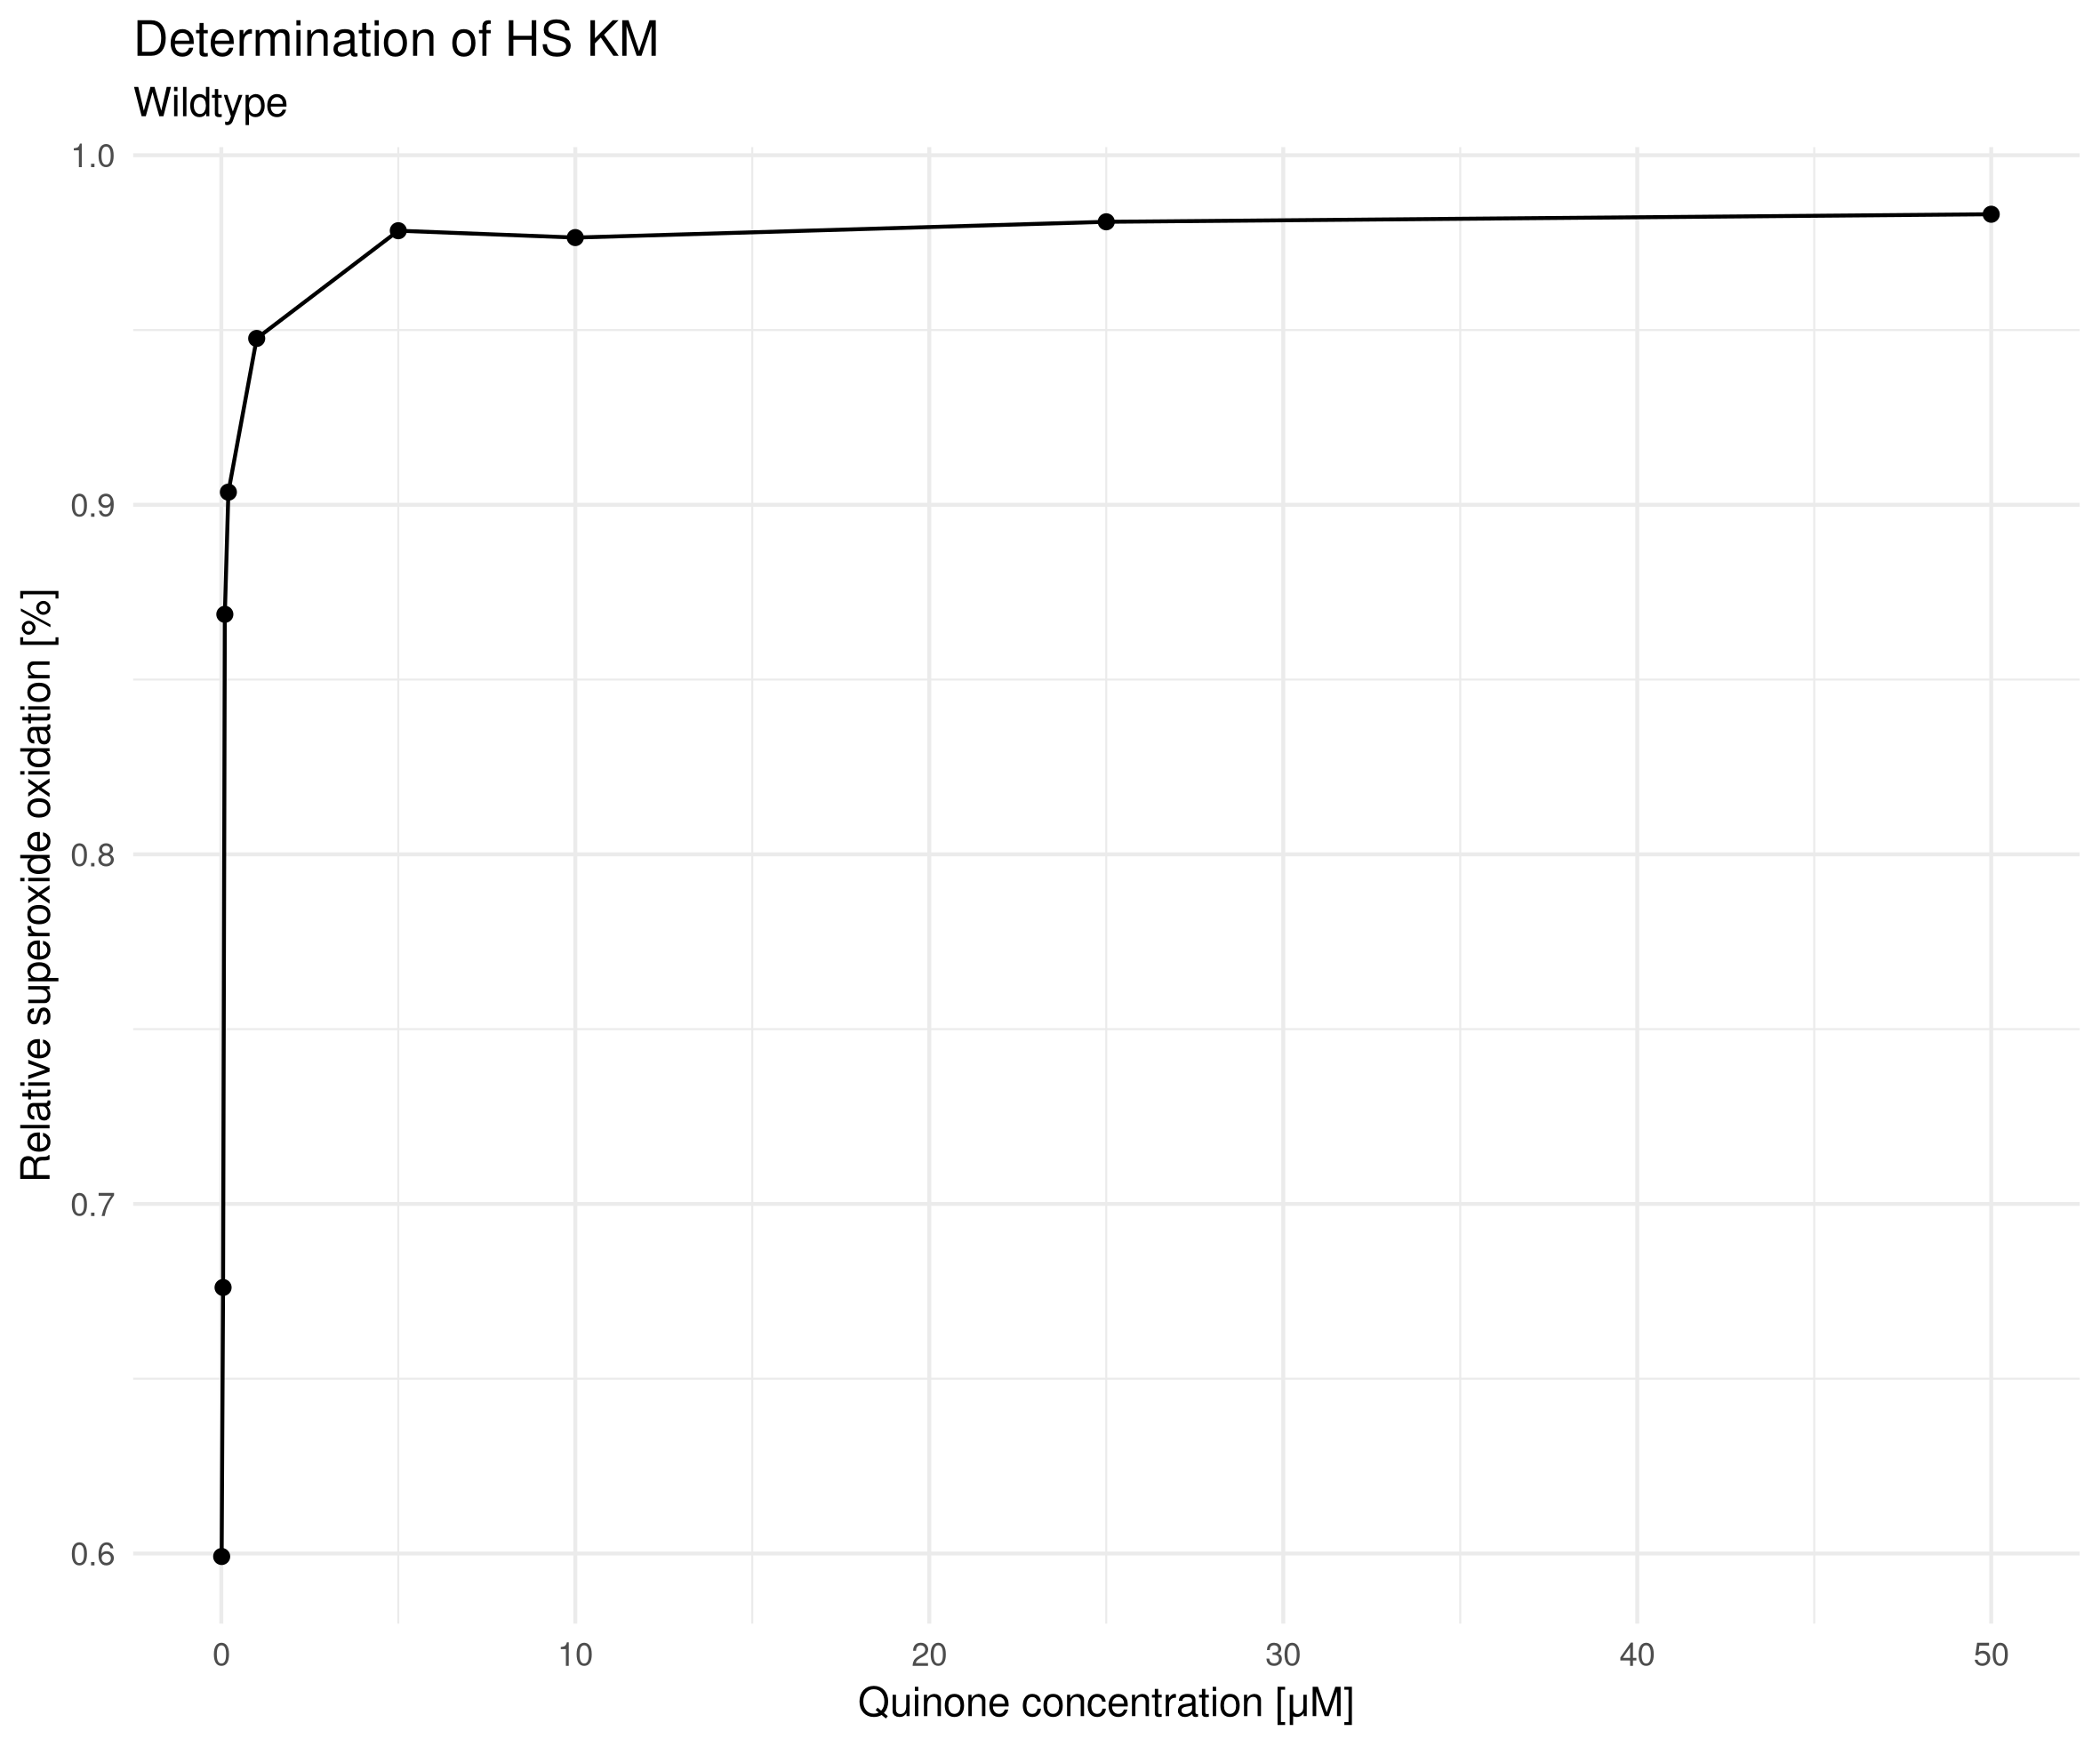
\includegraphics[width=\textwidth]{img/activity_wt_km.png}
	\caption{HS wildtype}
	\label{fig:activity_wt_km}
    \end{subfigure}
    \caption{Determination of relative superoxide oxidation per quinone concentration}
    \label{fig:activity_km}
\end{figure}

\begin{figure}
    \centering
    \begin{subfigure}{0.45\textwidth}
	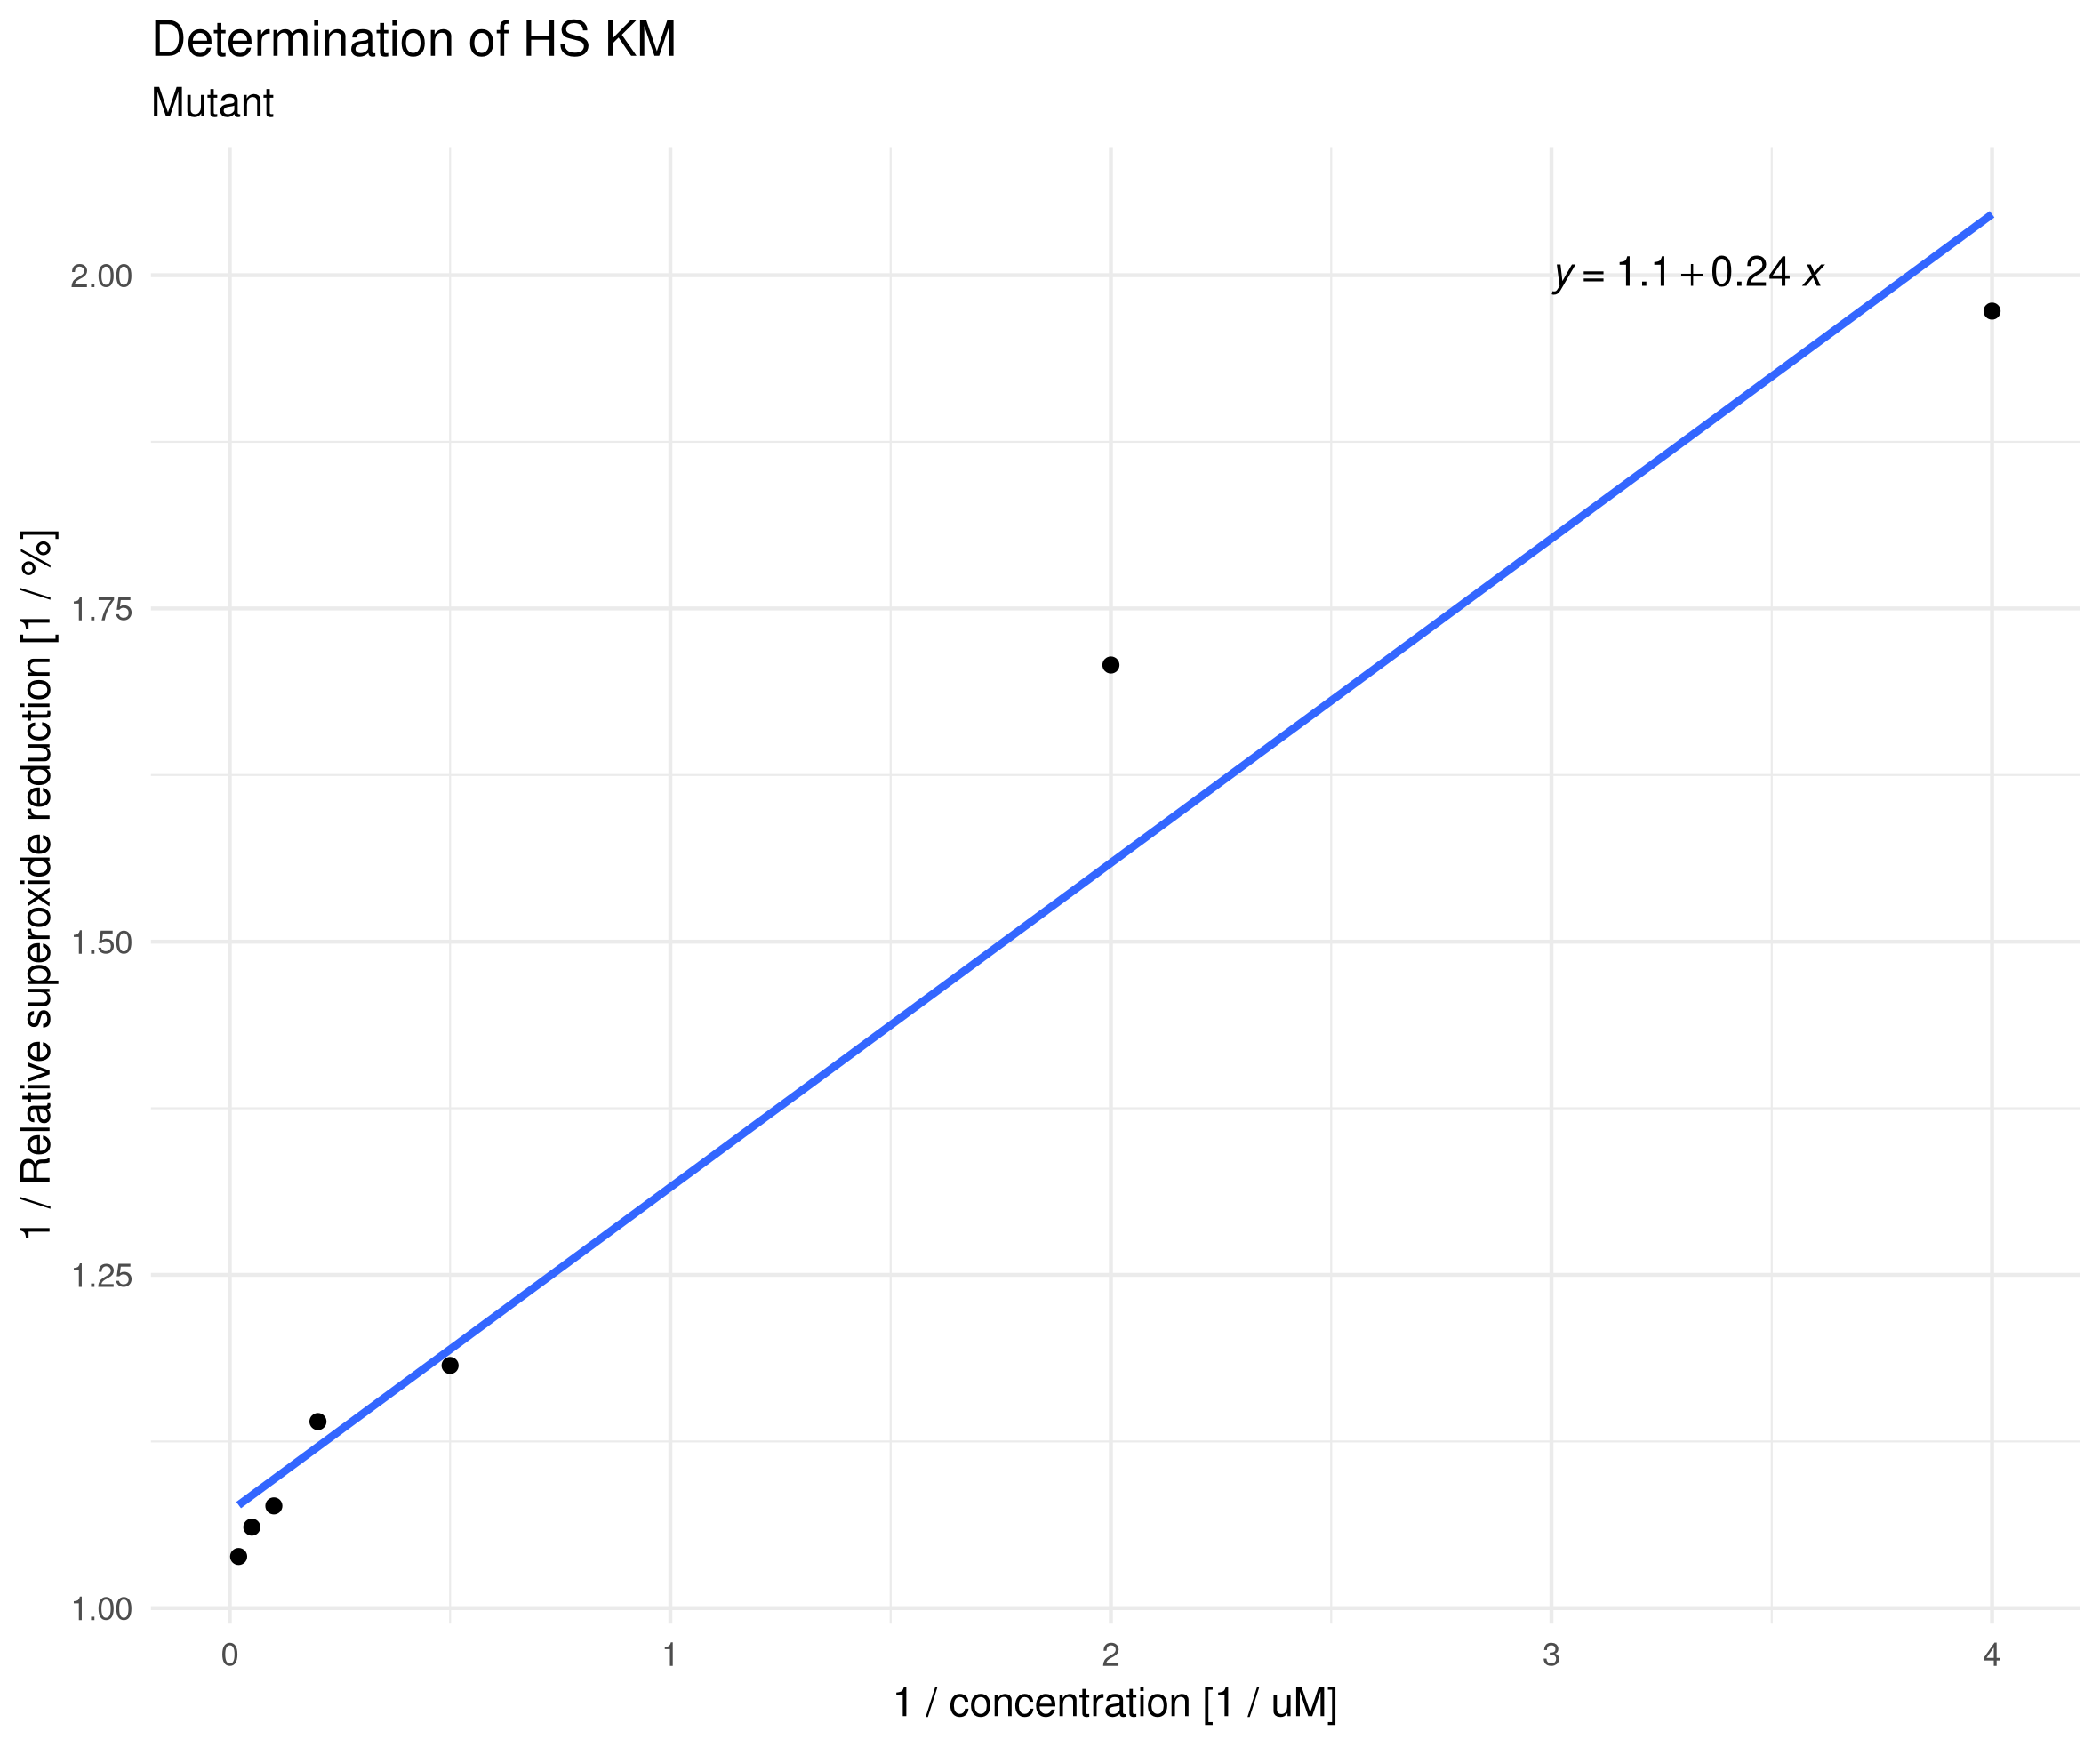
\includegraphics[width=\textwidth]{img/activity_mut_km_lb.png}
	\caption{HS mutant}
	\label{fig:activity_mut_km_lb}
    \end{subfigure}
    ~
    \begin{subfigure}{0.45\textwidth}
	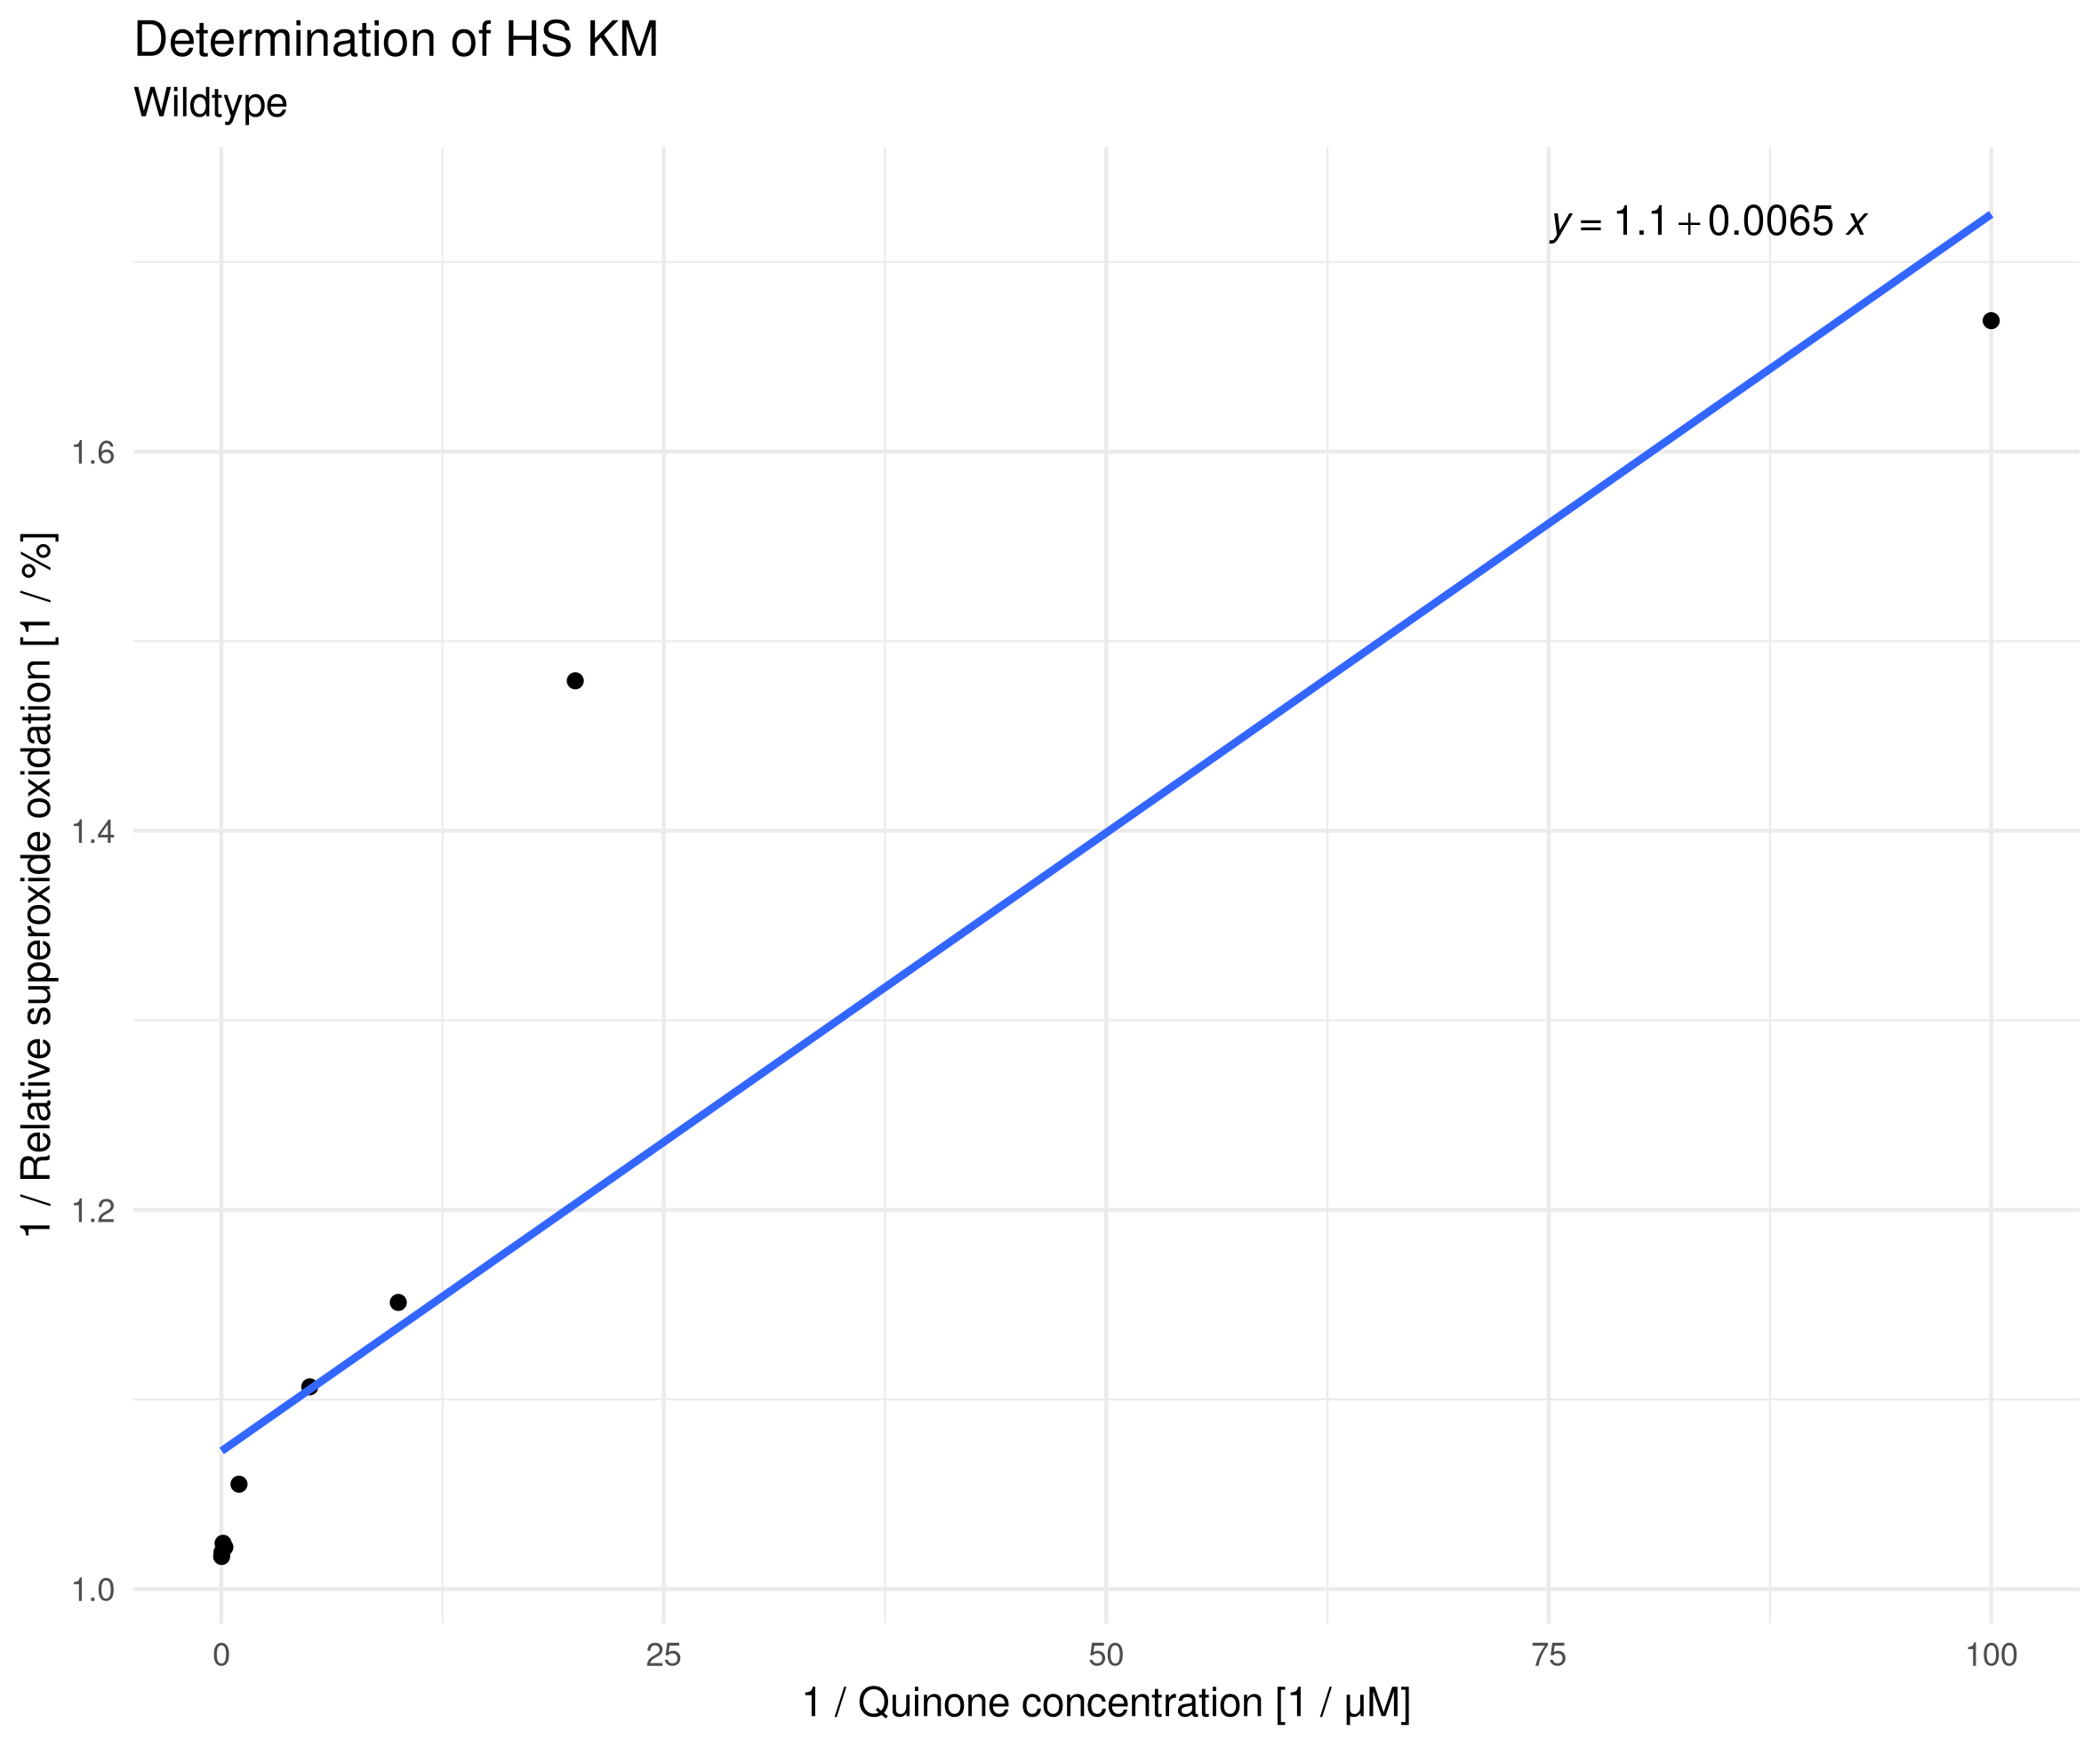
\includegraphics[width=\textwidth]{img/activity_wt_km_lb.png}
	\caption{HS wildtype}
	\label{fig:activity_wt_km_lb}
    \end{subfigure}
    \caption{Determination of $K_m$}
    \label{fig:activity_km_lb}
\end{figure}

\chapter{Discussion}

\section{Size exclusion chromatography}

In all three SEC graphs there are peaks next to the main one, which imply that
there were impurities within the column. Impurities which are in later
fractions than SOO took longer to pass through the columns, hence contain
molecules which are smaller than SOO. Similarly impurities which are in earlier
fractions are larger than SOO.

This step allowed to further purify the protein, allowing to filter not only on
the affinity to His-tagged nickel beads as was done before, but in addition to
filter based on the size of molecules.

\section{Protein concentration determination}

The determined concentration of the wild type and mutant is comparable, while
the one of dsRed is significantly bigger. This matches the observation that the
dsRed pellet at the beginning of purification was heavier.

\section{SDS PAGE}

\subsection{Purification}

\subsubsection{Flowthrough}

In all three samples the flowthrough contained many compounds of different
size. These were all compounds which were unable to bind to the column, hence
which did not have a His tag.

\subsubsection{Wash}

The wash samples of the wildtype and mutant did not contain a lot, whereas the
one of dsRed contained a variety of compounds found both in the flowthrough, as
well as in later stages. This might imply that the column used for dsRed had
been loaded above capacity.

\subsubsection{Wash \SI{5}{\milli\Molar}}

The \SI{5}{\milli\Molar} His wash allowed to wash out everything which was able
to weakly bind to the column, without washing out the strongly bound SOO.
Comparing the bands with the bands from later purification steps which are
known to be SOO imply that a bit of SOO was washed out in this step.

\subsubsection{Before ÄKTA}

The before ÄKTA lanes were the result of the elution of the column with
\SI{100}{\milli\Molar} His. The big bands are likely the HS. Of interest is
that, for the wildtype and mutant the big bands are around \SI{17}{\kilo\Da},
while for dsRed they are between \SIrange{43}{55}{\kilo\Da}. This implies that
the dsRed HS forms trimers, whose size would be around \SI{51}{\kilo\Da}. As
this behaviour is only seen in small amounts for the wildtype, and barely for
the mutant, dsRed itself seems to promote formation of these trimers.

To a lesser extent there are bands around \SI{34}{\kilo\Da} visible in all
three lanes, implying that all variants of HS form dimers to some extent.

\subsubsection{After ÄKTA}
The after ÄKTA lanes show that, while certain impurities were removed as in the
case of the mutant or dsRed, or at least had their concentration lowered as in
the case of the wildtype, a bit of HS was lost as well for all three proteins.

\subsection{dsRed cleavage}

Comparing the before ÄKTA lane with the before loading lane, between which the
sample was incubated with TEV protease, shows the lane around \SI{51}{\kilo\Da}
disappeared, while the one around \SI{17}{\kilo\Da}, known to be the band of
the HS wild type, got stronger. This implies that cleavage was successful.

There is an additional band visible slightly below \SI{26}{\kilo\Da}, which can
be identifies as the TEV protease by comparing it with the lane where only TEV
protease was loaded.

The flowthrough only contains HS at \SI{17}{\kilo\Da}, which is expected as
both the TEV protease as well as dsRed are His-tagged, so will have stayed
bound to the column. Similarly the elution then contained bands which
correspond with the TEV protease.

\section{Fluorescence measurements}

\subsection{Membrane extraction}

In the first step where cells were cracked open in the maximator there were
barely any losses of proteins. This is to be expected as care was taken to not
discard any proteins left inside the maximator.

The ultracentrifugation step seems to have already lead to significant losses
though, hinting that either there were still some membranes left in solution
rather than in the pellet, or parts of the pellet had been lost. One approach
to try and lower these losses would be to centrifuge for longer, or potentially
multiple times.

\subsection{Affinity chromatrography}

As the fluoroescence of the flowthrough was comparably high it would seem that
too much protein was loaded onto the column, so some was unable to bind. This
also matches the observation for the corresponding sample in the SDS-PAGE gel
mentioned above. This lead to some losses of proteins.

The wash step with plain buffer did not seem to cause any significant loss of
proteins, while the one with \SI{5}{\milli\Molar} Hist did cause the early
elution of some proteins. This might be hard to avoid as some His-tagged
protein is guaranteed to bind to the wash buffer.

The fluorescence of the elution, when compared to the fluoroescence of the last
step of the membrane extraction, then shows that not too much protein was lost
during the affinity chromatography.

\subsection{Reverse IMAC}

The fluorescence of the elution and flowthrough stages confirms what was
already seen in the SDS-PAGE gel - the majority of the fluorescent dsRed was
in the elution, so bound to the column. Only a small part was in the
flowthrough, which might eg be dsRed which was washed out by the
\SI{5}{\milli\Molar} His wash buffer.

\section{Relative enzyme reduction}

For both quinol and superoxide the negative control confirms that the change in
absorbance was caused by the reduction of HS, and not by something unrelated.
In either case are the relative reductions of the wild type and mutant
comparable, implying that the mutation does not have a direct effect on the
equilibrium.

\subsection{Superoxide as substrate}

The relative reduction of samples where SOD was added clearly shows that SOD is
able to quench the reduction of HS, by quickly removing superoxide from the
system.

The data shows that the relative reduction of solubilized enzymes is
significantly higher than those of reconstituted enzymes. This might imply that
superoxide is unable to enter liposomes, such that in the case of liposomes it
cannot reduce those HS enzymes whose active site is within the liposome. Such
an observation was also made in the one of the referenced papers \cite{soo}.
Under the assumption that this holds we can estimate, by comparing the relative
reduction of reconstituted and solubilized enzymes, that in liposomes about
half the enzymes have one orientation, while the other half has another.

\subsection{Quinol as substrate}

The reduction of the reconstituted HS is close to the theoretical maximum of
\SI{50}{\percent}, as only one of the two Hems can be reduced by quinol
addition. Of interest is that the relative reduction of solubilized HS is
significantly lower than that of the reconstituted. This might either be an
experimental error which further experiments could clarify, or quinol has an
easier time binding to reconstituted enzymes over solubilized ones.

\section{Fluorescence measurements before and after cleavage}

\subsection{Solubilized dsRed}

The measurements with solubilized dsRed served to show that the method works.
There is clear fluorescence in the first measurement, which can be quenched
significantly by adding copper, and restored by adding the chelating agent
EDTA.

\subsection{Uncleaved liposomes}

The exact same behaviour can be observed with uncleaved liposomes. As
fluorescence is heavily quenched upon adding a lot of copper one can assume
that the vast majority, if not all, dsRed is oriented towards the outside of
the liposome. The remaining bit of fluorescence might either be dsRed which is
oriented towards the inside of the liposome, or a lacking amount of copper
added. This can also be seen in the second measurement with a higher volume of
liposomes, where not all fluoroescence could be quenched.

\subsection{Cleaved liposomes}

With cleaved liposomes there was a significantly lower initial fluorescence
compared with uncleaved ones. This confirms that cleavage itself was a success.
As this fluorescence can be quenched with copper, however, there must be
uncleaved dsRed left oriented towards the outside of the liposomes, as copper
cannot enter those. This implies that cleavage was not complete, and a longer
incubation or higher concentration of TEV protease would be needed.

\section{Activity measurement}

The equal to within rounding limits $v_{\text{max}}$ imply that the mutation
does not impede the maximum speed of the enzyme in case of an overwhelming
substrate concentration. The $K_m$ values however, which differ by two orders
of magnitude, imply that the mutation significantly lowers the affinity of the
enzyme for quinone, lowering its speed in a system with low substrate
concentration.


\bibliographystyle{plain}
\bibliography{references}

\end{document}



